Após a execução do Script de codificação, os dados obtidos são armazenados
em um arquivo CSV. Com os resultados finais, outro script em \textit{Python} é
executado, onde ele cria um gráfico com estes dados. Abaixo estão os resultados
obtidos.

A análise dos gráficos gerados para as sequências testadas permite observar o comportamento 
do \acrshort{LCEVC} em diferentes condições de codificação. Foram analisados dois
codificadores: \acrshort{AVC} e \acrshort{VVC}, com e sem o uso do \acrshort{LCEVC} 
como camada de aprimoramento.

No geral, os gráficos \acrshort{PSNR} x Taxa de bits permitem avaliar a eficiência da
compressão, considerando que uma melhor relação é obtida quando se atinge maior qualidade
(\acrshort{PSNR}) com menor taxa de bits. A seguir, apresenta-se uma
análise detalhada por cenário. Para alguns resultados, se um vídeo em \acrshort{LCEVC} 
resultou em uma taxa de bits muito alta, ficando distante dos valores
do codificador base, eles foram omitidos para melhor análise e visualização nos gráficos.

Além disso, para que o gráfico pudesse ficar legível, só foi rotulado o valor de SW2 para
o parâmetro de QP37.

\newpage
\section{AVC}

\subsection{Bosphorus}
\begin{figure}[h]
    \centering
    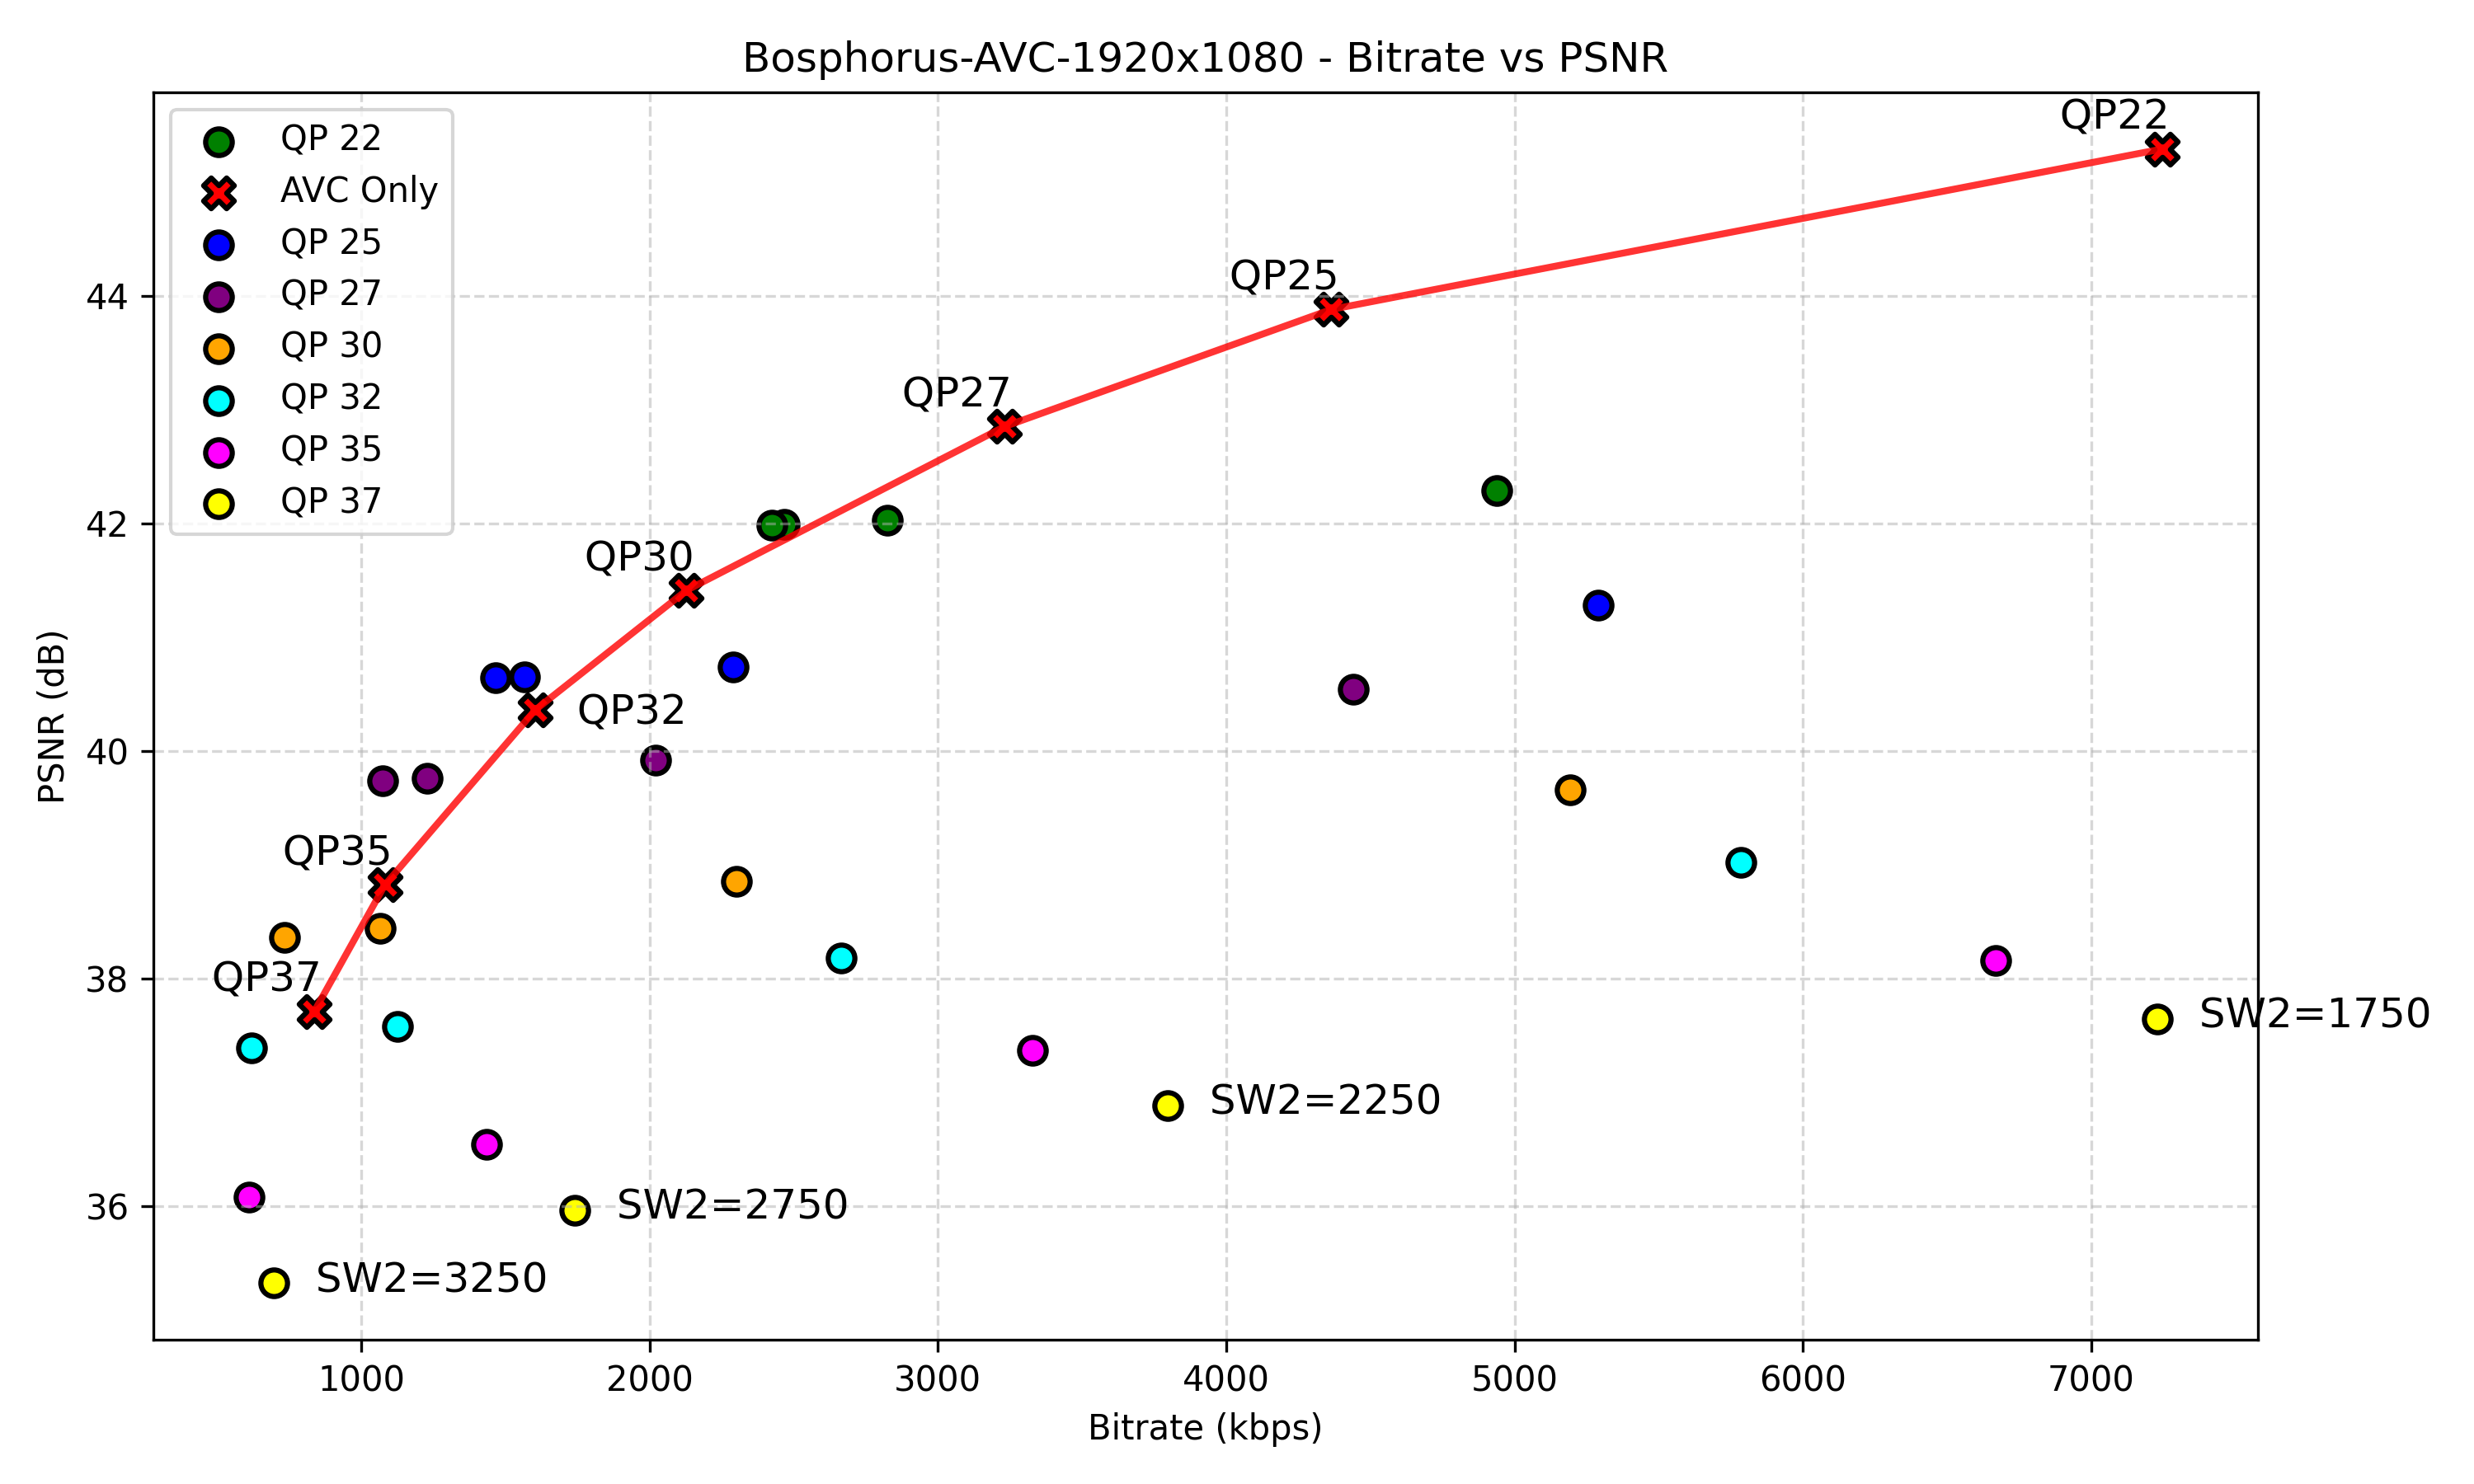
\includegraphics[width=1.0\textwidth]{img/Bosphorus-AVC.png}
    \caption{Resultados para "Bosphorus"\ em \acrshort{AVC}. \cite{uvg_dataset}}
    \label{fig:bosphorus}
\end{figure}

Para a sequência Bosphorus, o \acrshort{LCEVC} conseguiu ótimos resultados. Mesmo
com uma grande dispersão pela tabela e vários resultados ineficientes, certos valores
de SW2 conseguiram atingir resultados positivos.

Para o \acrshort{LCEVC}, vemos resultados positivos para QP 30, 27, 25 e 22. Estes
QPs conseguiram resultados superiores à curva de eficiência dos vídeos de referência.
Os resultados que apresentaram um resultado superior ao \acrshort{AVC} estão abaixo.

\begin{table}[h]
    \centering
    \begin{tabular}{|c|c|c|c|}
        \hline
        \textbf{QP} & \textbf{Tamanho (b)} & \textbf{PSNR (dB)} & \textbf{Taxa (kbps)} \\
        \hline
        37 & 1047004 & 37.71 & 837.60 \\
        35 & 1352315 & 38.82 & 1081.85 \\
        32 & 2005088 & 40.36 & 1604.07 \\
        30 & 2660081 & 41.41 & 2128.06 \\
        27 & 4038641 & 42.85 & 3230.91 \\
        25 & 5455551 & 43.88 & 4364.44 \\
        22 & 9055951 & 45.29 & 7244.76 \\
        \hline
    \end{tabular}
    \caption{Resultados para Bosphorus em AVC.}
    \label{tab:bosphorus-avc}
\end{table}

\begin{table}[h]
    \centering
    \label{tab:bosphorus-avc-lcevc}
    \begin{tabular}{|c|c|c|c|c|c|c|c|}
        \hline
        \textbf{SW2} & \textbf{QP} & \textbf{Tamanho (b)} & \textbf{Proporção} & \textbf{PSNR (dB)} & \textbf{Taxa (kbps)} & \textbf{Superou} \\
        \hline
        3250 & 30 & 916195 & 10.03\% & 38.36 & 732.96 & AVC QP37\\
        3250 & 27 & 1342845 & 2.68\% & 39.74 & 1074.28 & AVC QP35\\
        2750 & 27 & 1536124 & 14.93\% & 39.76 & 1228.90 & AVC QP35\\
        3250 & 25 & 1831695 & 2.30\% & 40.64 & 1465.36 & AVC QP32\\
        2750 & 25 & 1958104 & 8.61\% & 40.65 & 1566.48 & AVC QP32\\
        3250 & 22 & 3031413 & 1.21\% & 41.98 & 2425.13 & AVC QP30-27\\
        2750 & 22 & 3083003 & 2.86\% & 41.99 & 2466.40 & AVC QP30-27\\
        \hline
    \end{tabular}
    \caption{Resultados favoráveis do LCEVC para Bosphorus em AVC}
\end{table}

Estes resultados mostram cenários onde o \acrshort{LCEVC} se mostrou superior ao uso de somente
\acrshort{AVC} e o respectivo resultado que ele superou.
 
\subsection{ReadySteadyGo}

\begin{figure}[h]
    \centering
    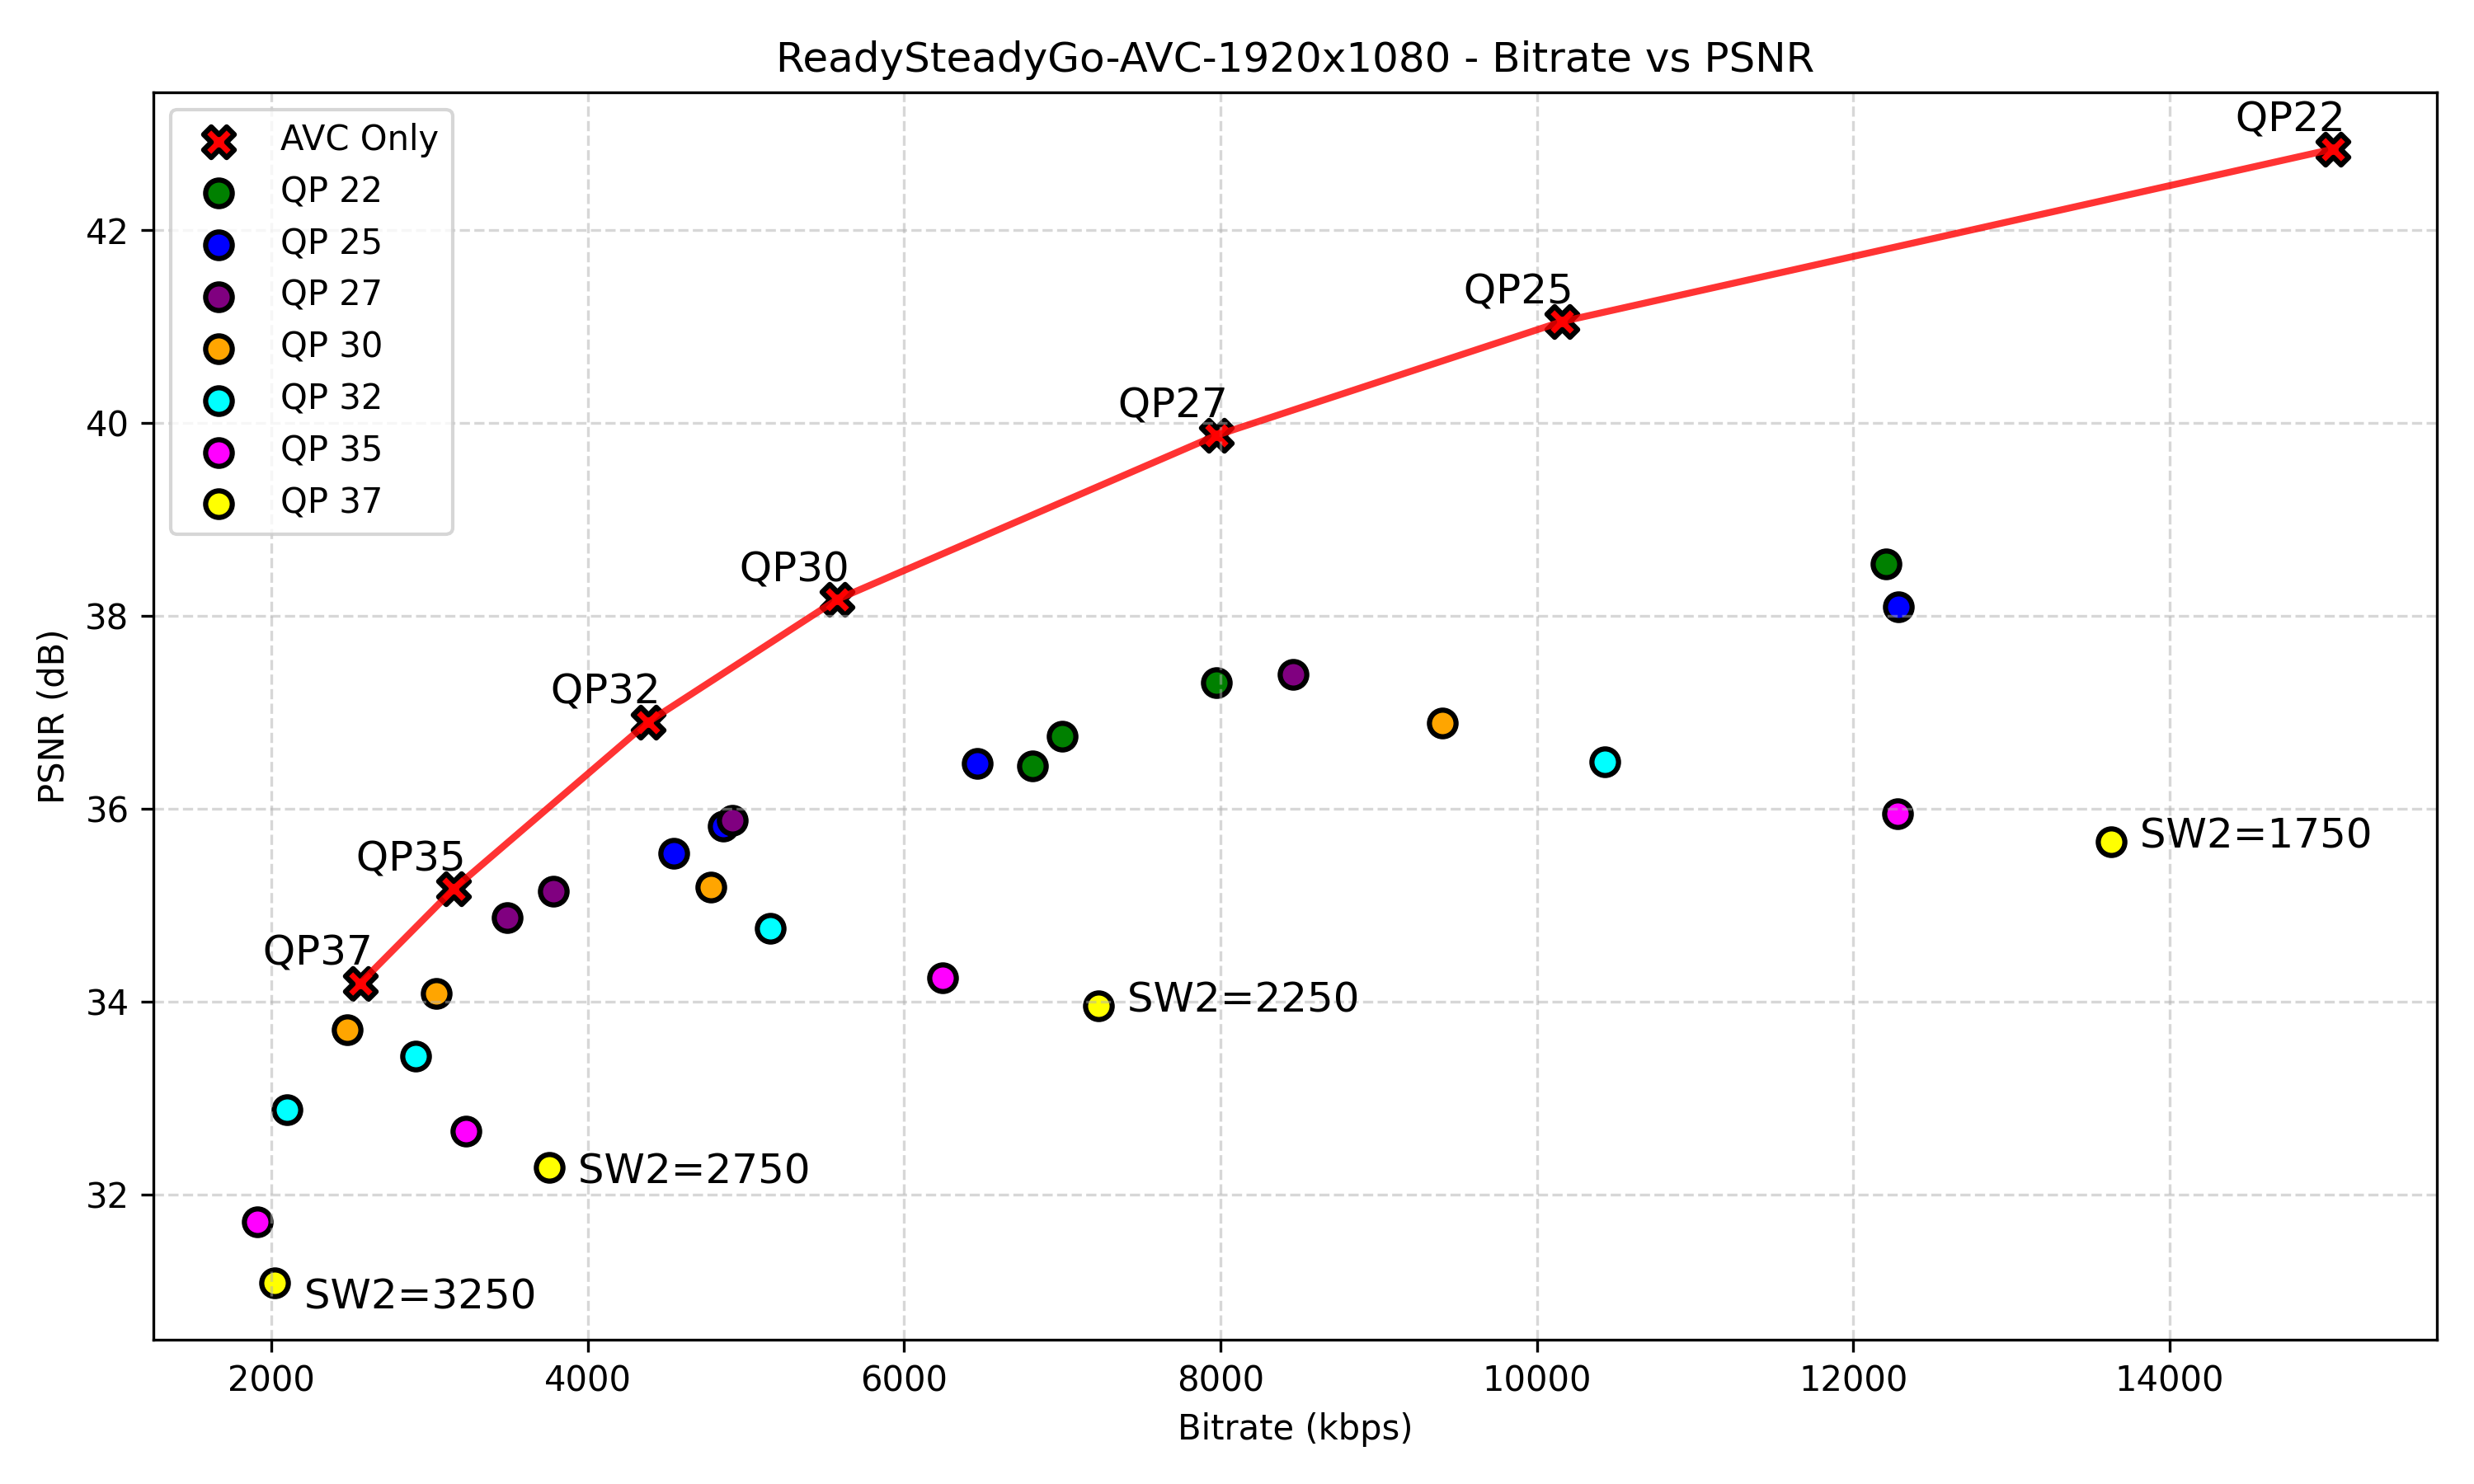
\includegraphics[width=1.0\textwidth]{img/ReadySteadyGo-AVC.png}
    \caption{Resultados para "ReadySteadyGo"\ em \acrshort{AVC}. \cite{uvg_dataset}}
    \label{fig:RSG}
\end{figure}

Para esta sequência, o \acrshort{LCEVC} não conseguiu atingir resultados satisfatórios.
Todos os seus resultados foram abaixo da curva do \acrshort{AVC} e não mostrou resultados
que justifiquem o seu uso baseado em melhora de qualidade ou taxa. Porém, os resultados
para um SW2 maior, ficaram relativamente próximos, como é o caso do QP 30 e 27 do \acrshort{LCEVC}.
Nestes casos, o uso do \acrshort{LCEVC} manteria o \acrshort{PSNR} próximo ao resultado
obtido para a referência em QP 37 e 35, onde, por exemplo, o uso do \acrshort{LCEVC} para se adequar a 
um novo padrão não seria perceptível.


\subsection{Jockey}

\begin{figure}[h]
    \centering
    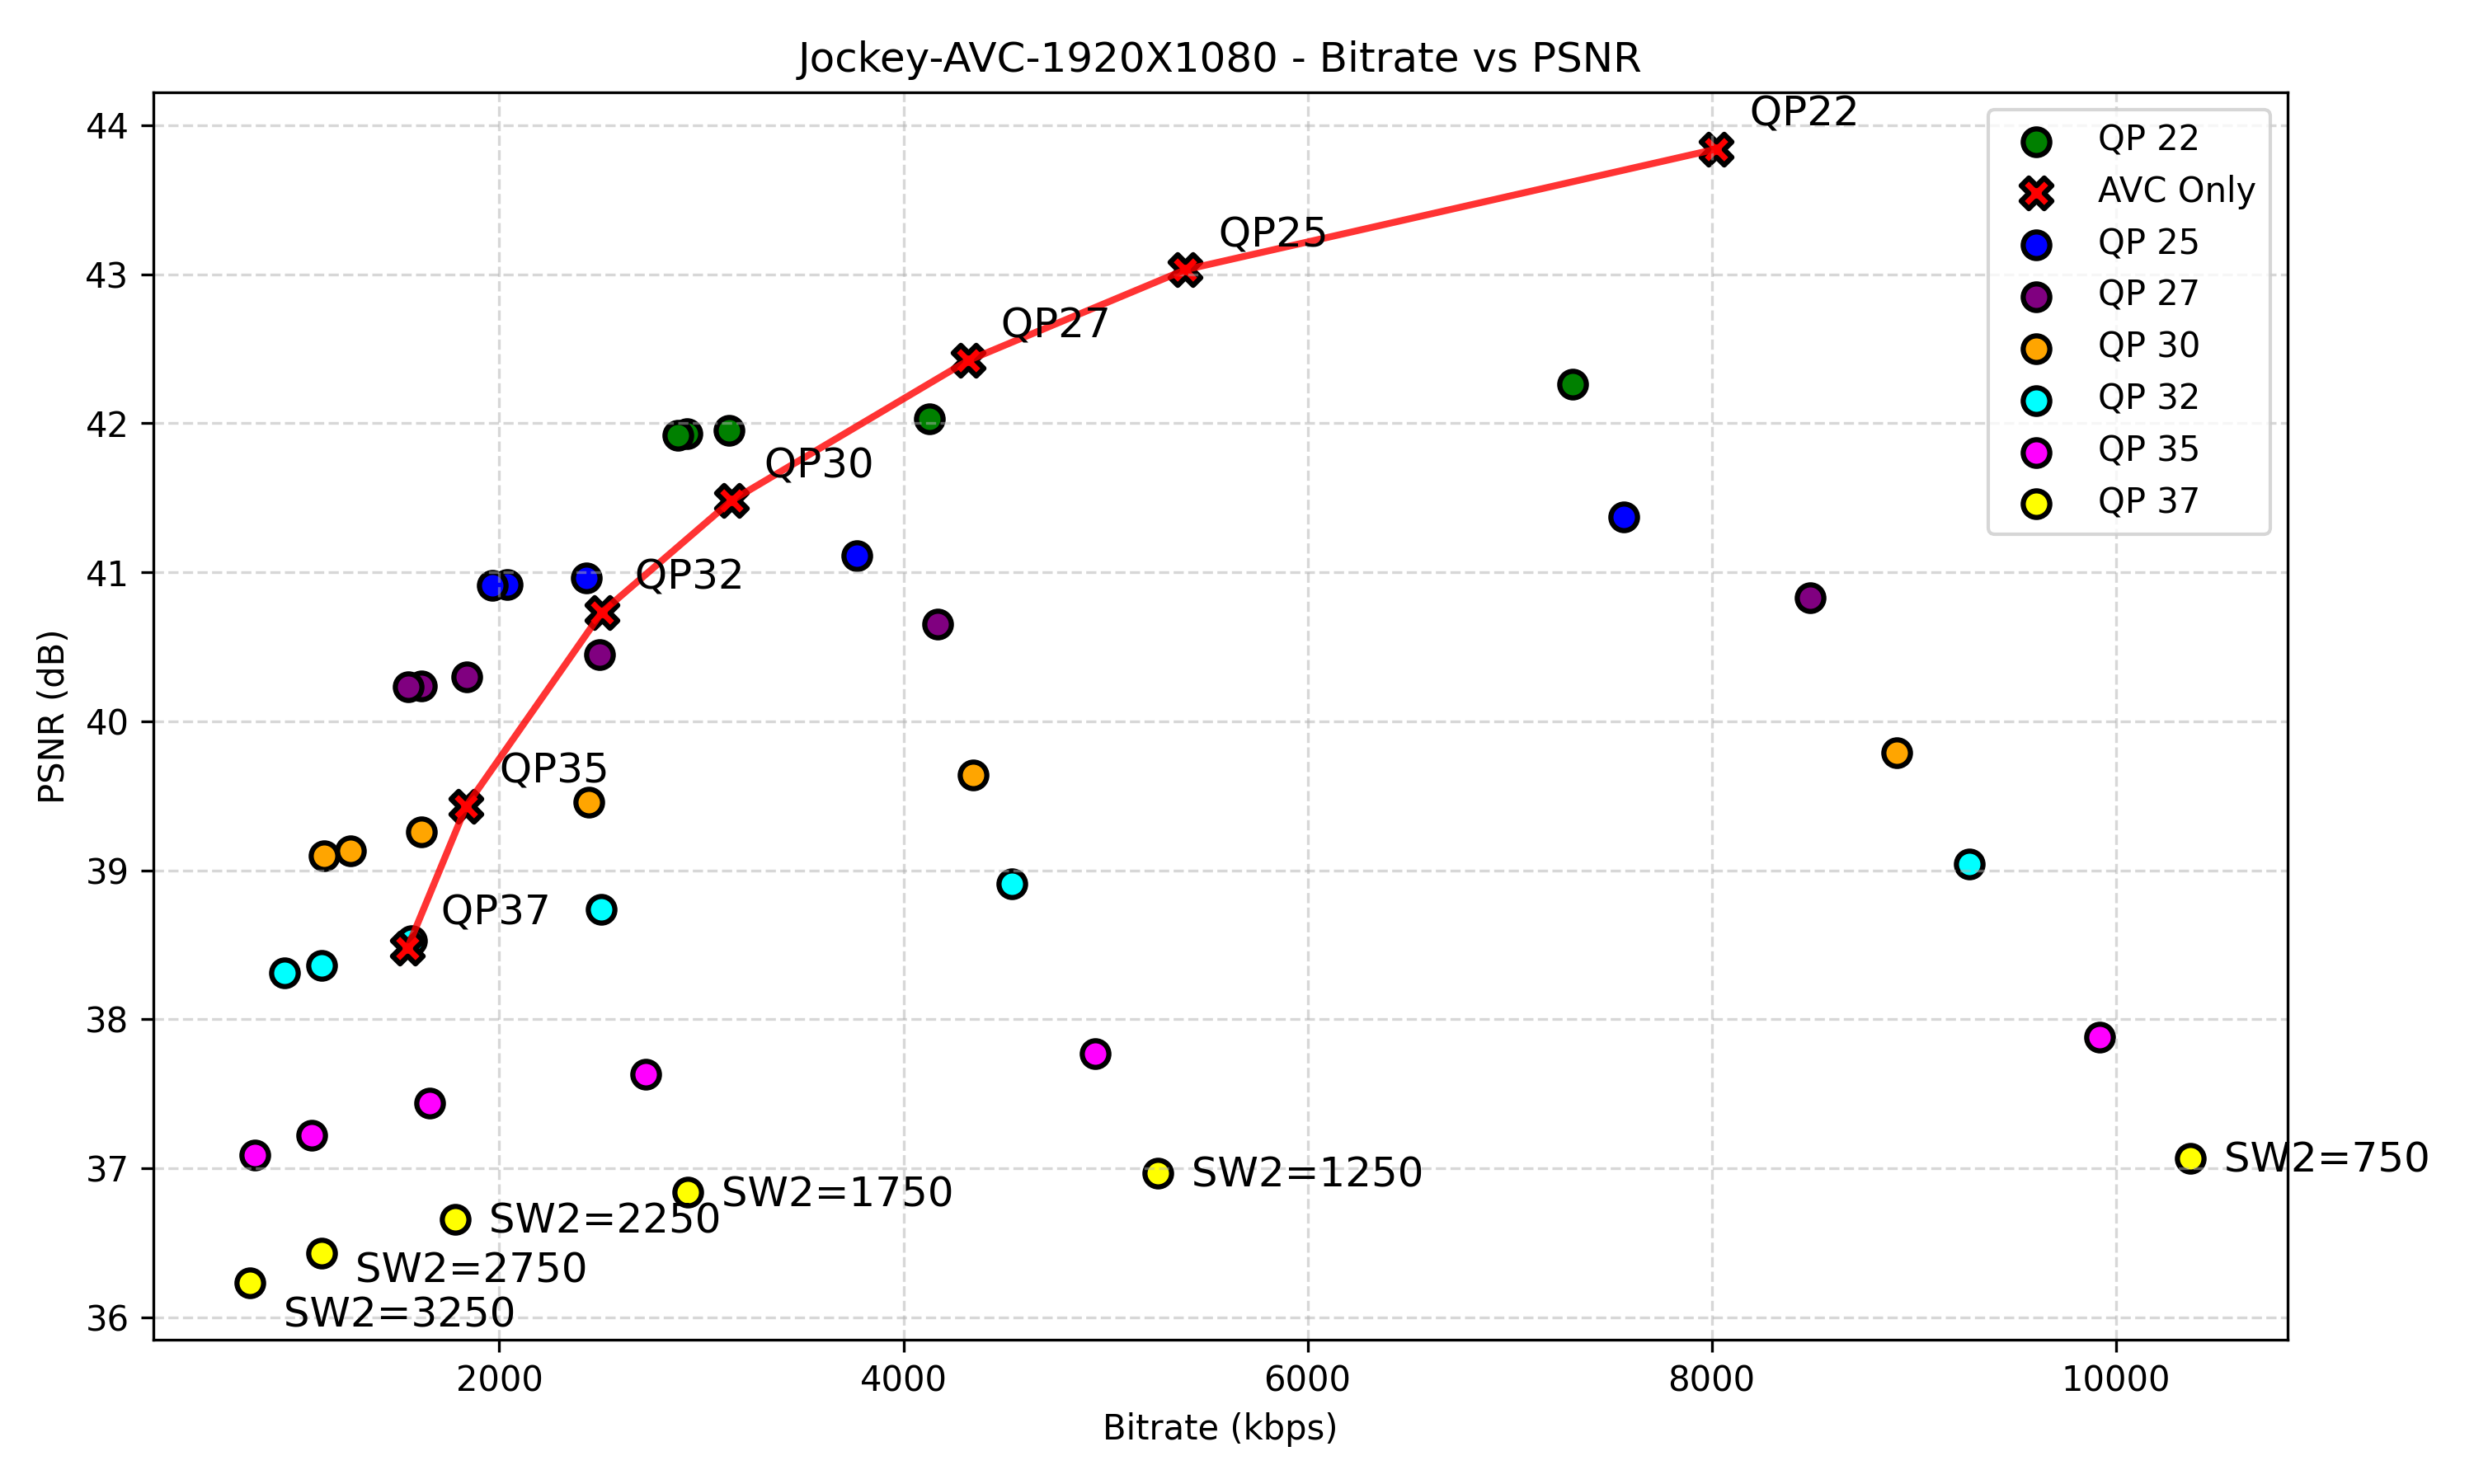
\includegraphics[width=1.0\textwidth]{img/Jockey-AVC.png}
    \caption{Resultados para "Jockey"\ em \acrshort{AVC}. \cite{uvg_dataset}}
    \label{fig:Jockey}
\end{figure}

Aqui é outro caso onde o \acrshort{LCEVC} obteve resultados satisfatórios. Vários resultados
estão acima da curva do \acrshort{AVC}, demonstrando uma ótima performance o \acrshort{LCEVC}
para os parâmetros escolhidos. Os valores de QP para \acrshort{LCEVC} que se destacaram foram
32, 30, 27 e 25, que ficaram acima da curva de referência.
Agora, levando em consideração somente os pontos que estão acima
dos pontos do \acrshort{AVC}, temos o seguinte resultado.

\begin{table}[h]
    \centering
    \begin{tabular}{|c|c|c|c|}
        \hline
        \textbf{QP} & \textbf{Tamanho (b)} & \textbf{PSNR (dB)} & \textbf{Taxa (kbps)} \\
        \hline
        37 & 1932479 & 38.48 & 1545.98 \\
        35 & 2294827 & 39.43 & 1835.86 \\
        32 & 3132841 & 40.73 & 2506.27 \\
        30 & 3935452 & 41.48 & 3148.36 \\
        27 & 5398380 & 42.42 & 4318.70 \\
        25 & 6743403 & 43.03 & 5394.72 \\
        22 & 10029224 & 43.84 & 8023.38 \\
        \hline
    \end{tabular}
    \caption{Resultados para Jockey em AVC.}
    \label{tab:jockey-avc}
\end{table}

\begin{table}[h]
    \centering
    \label{tab:jockey-avc-lcevc}
    \begin{tabular}{|c|c|c|c|c|c|c|c|}
        \hline
        \textbf{SW2} & \textbf{QP} & \textbf{Tamanho (b)} & \textbf{Proporção} & \textbf{PSNR (dB)} & \textbf{Taxa (kbps)} & \textbf{Superou} \\
        \hline
            2250 & 32 & 1955243 & 45.60\% & 38.53 & 1564.19 & AVC QP37\\
            3250 & 30 & 1417144 & 4.45\% & 39.10 & 1133.72 & AVC QP37 \\
            2750 & 30 & 1580745 & 14.34\% & 39.13 & 1264.60 & AVC QP37 \\
            2250 & 30 & 2019083 & 32.94\% & 39.26 & 1615.27 & AVC QP37 \\
            3250 & 27 & 1934343 & 1.69\% & 40.23 & 1547.47 & AVC QP35 \\
            2750 & 27 & 2017641 & 5.75\% & 40.24 & 1614.11 & AVC QP35 \\
            2250 & 27 & 2298071 & 17.25\% & 40.30 & 1838.46 & AVC QP35 \\
            3250 & 25 & 2455423 & 1.78\% & 40.91 & 1964.34 & AVC QP32\\
            2750 & 25 & 2549768 & 5.41\% & 40.92 & 2039.81 & AVC QP32\\
            2250 & 25 & 3036843 & 20.58\% & 40.96 & 2429.47 & AVC QP32\\
            3250 & 22 & 3603619 & 1.11\% & 41.92 & 2882.90 & AVC QP30 \\
            2750 & 22 & 3658403 & 2.59\% & 41.93 & 2926.72 & AVC QP30 \\
            2250 & 22 & 3923132 & 9.16\% & 41.95 & 3138.51 & AVC QP30 \\
        \hline
    \end{tabular}
    \caption{Resultados favoráveis do LCEVC para Jockey em AVC.}
\end{table}

\subsection{SOCCER}

\begin{figure}[h]
    \centering
    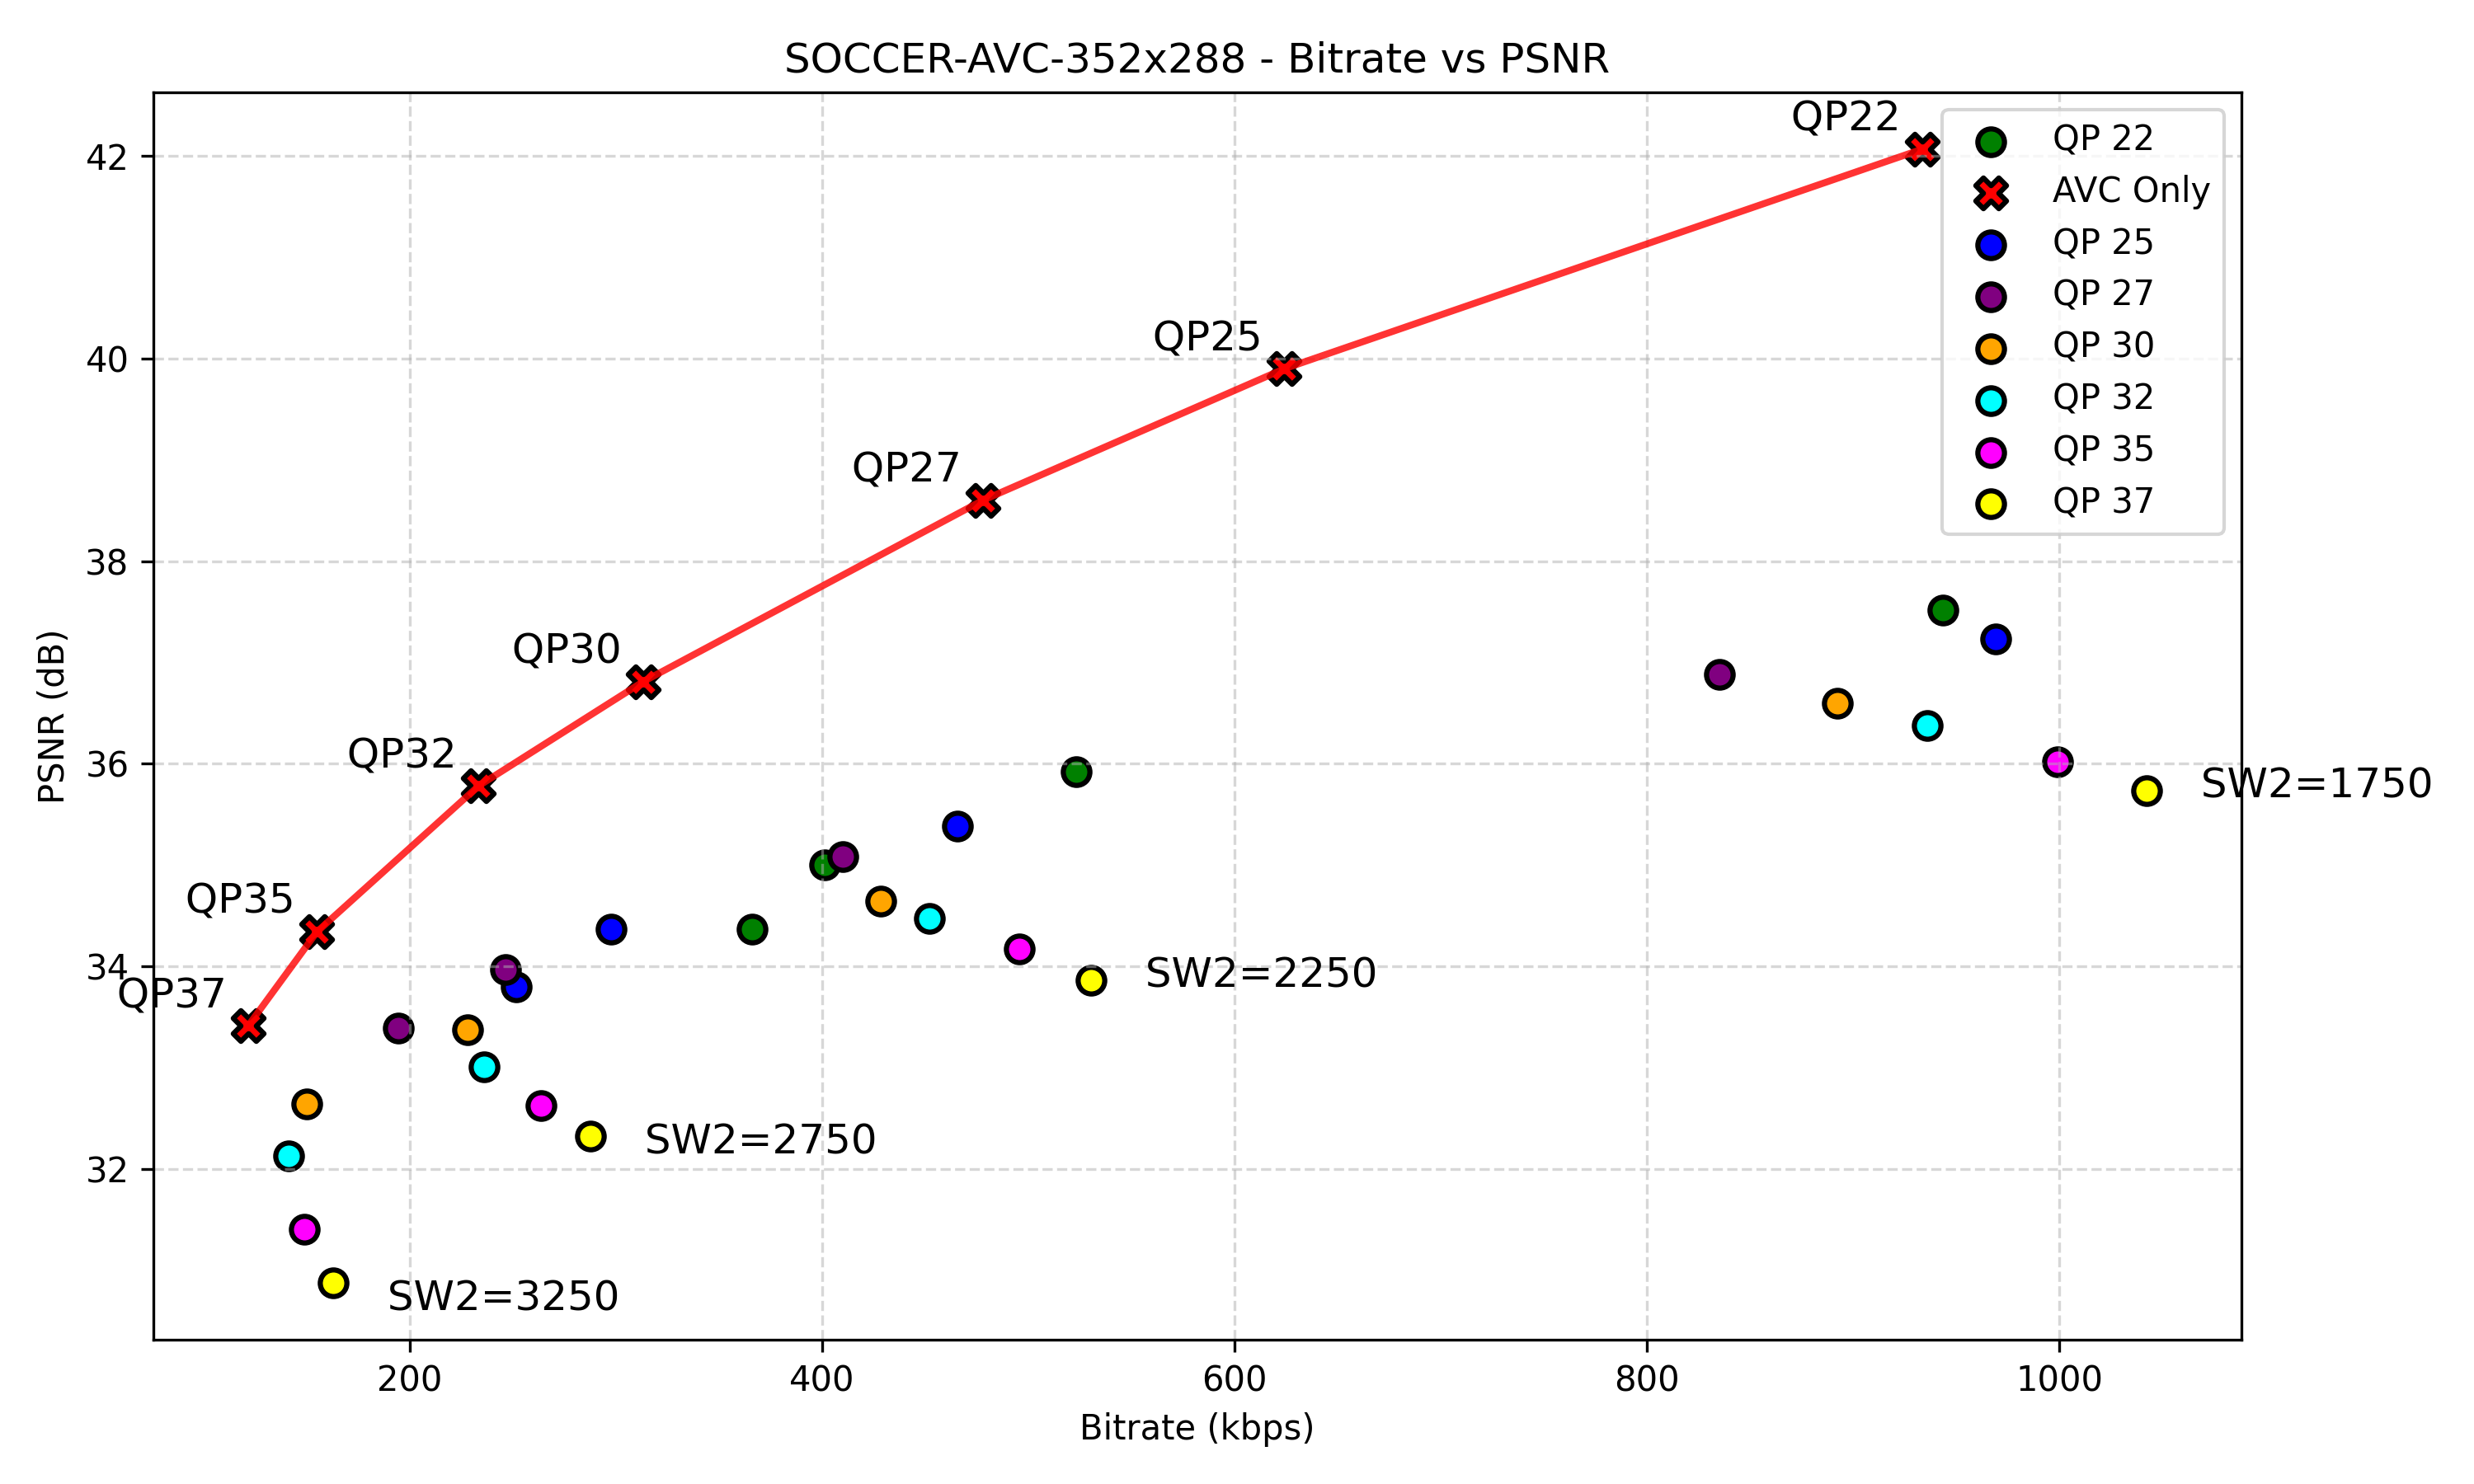
\includegraphics[width=0.85\textwidth]{img/SOCCER-AVC.png}
    \caption{Resultados para "SOCCER"\ em \acrshort{AVC}. \cite{xiph}}
    \label{fig:SOCCER}
\end{figure}

Os resultados indicam que o \acrshort{LCEVC} não apresentou vantagem clara em relação
a somente o \acrshort{AVC} na maioria das configurações testadas. Para esta sequência 
com uma resolução menor, ele não conseguiu atingir resultados satisfatórios. Assim,
não houve benefícios em utilizar o \acrshort{LCEVC} com \acrshort{AVC} nesta sequência,
pois os resultados usando somente o \acrshort{AVC} já obteram o melhor resultado.  

\newpage
\subsection{City}

\begin{figure}[h]
    \centering
    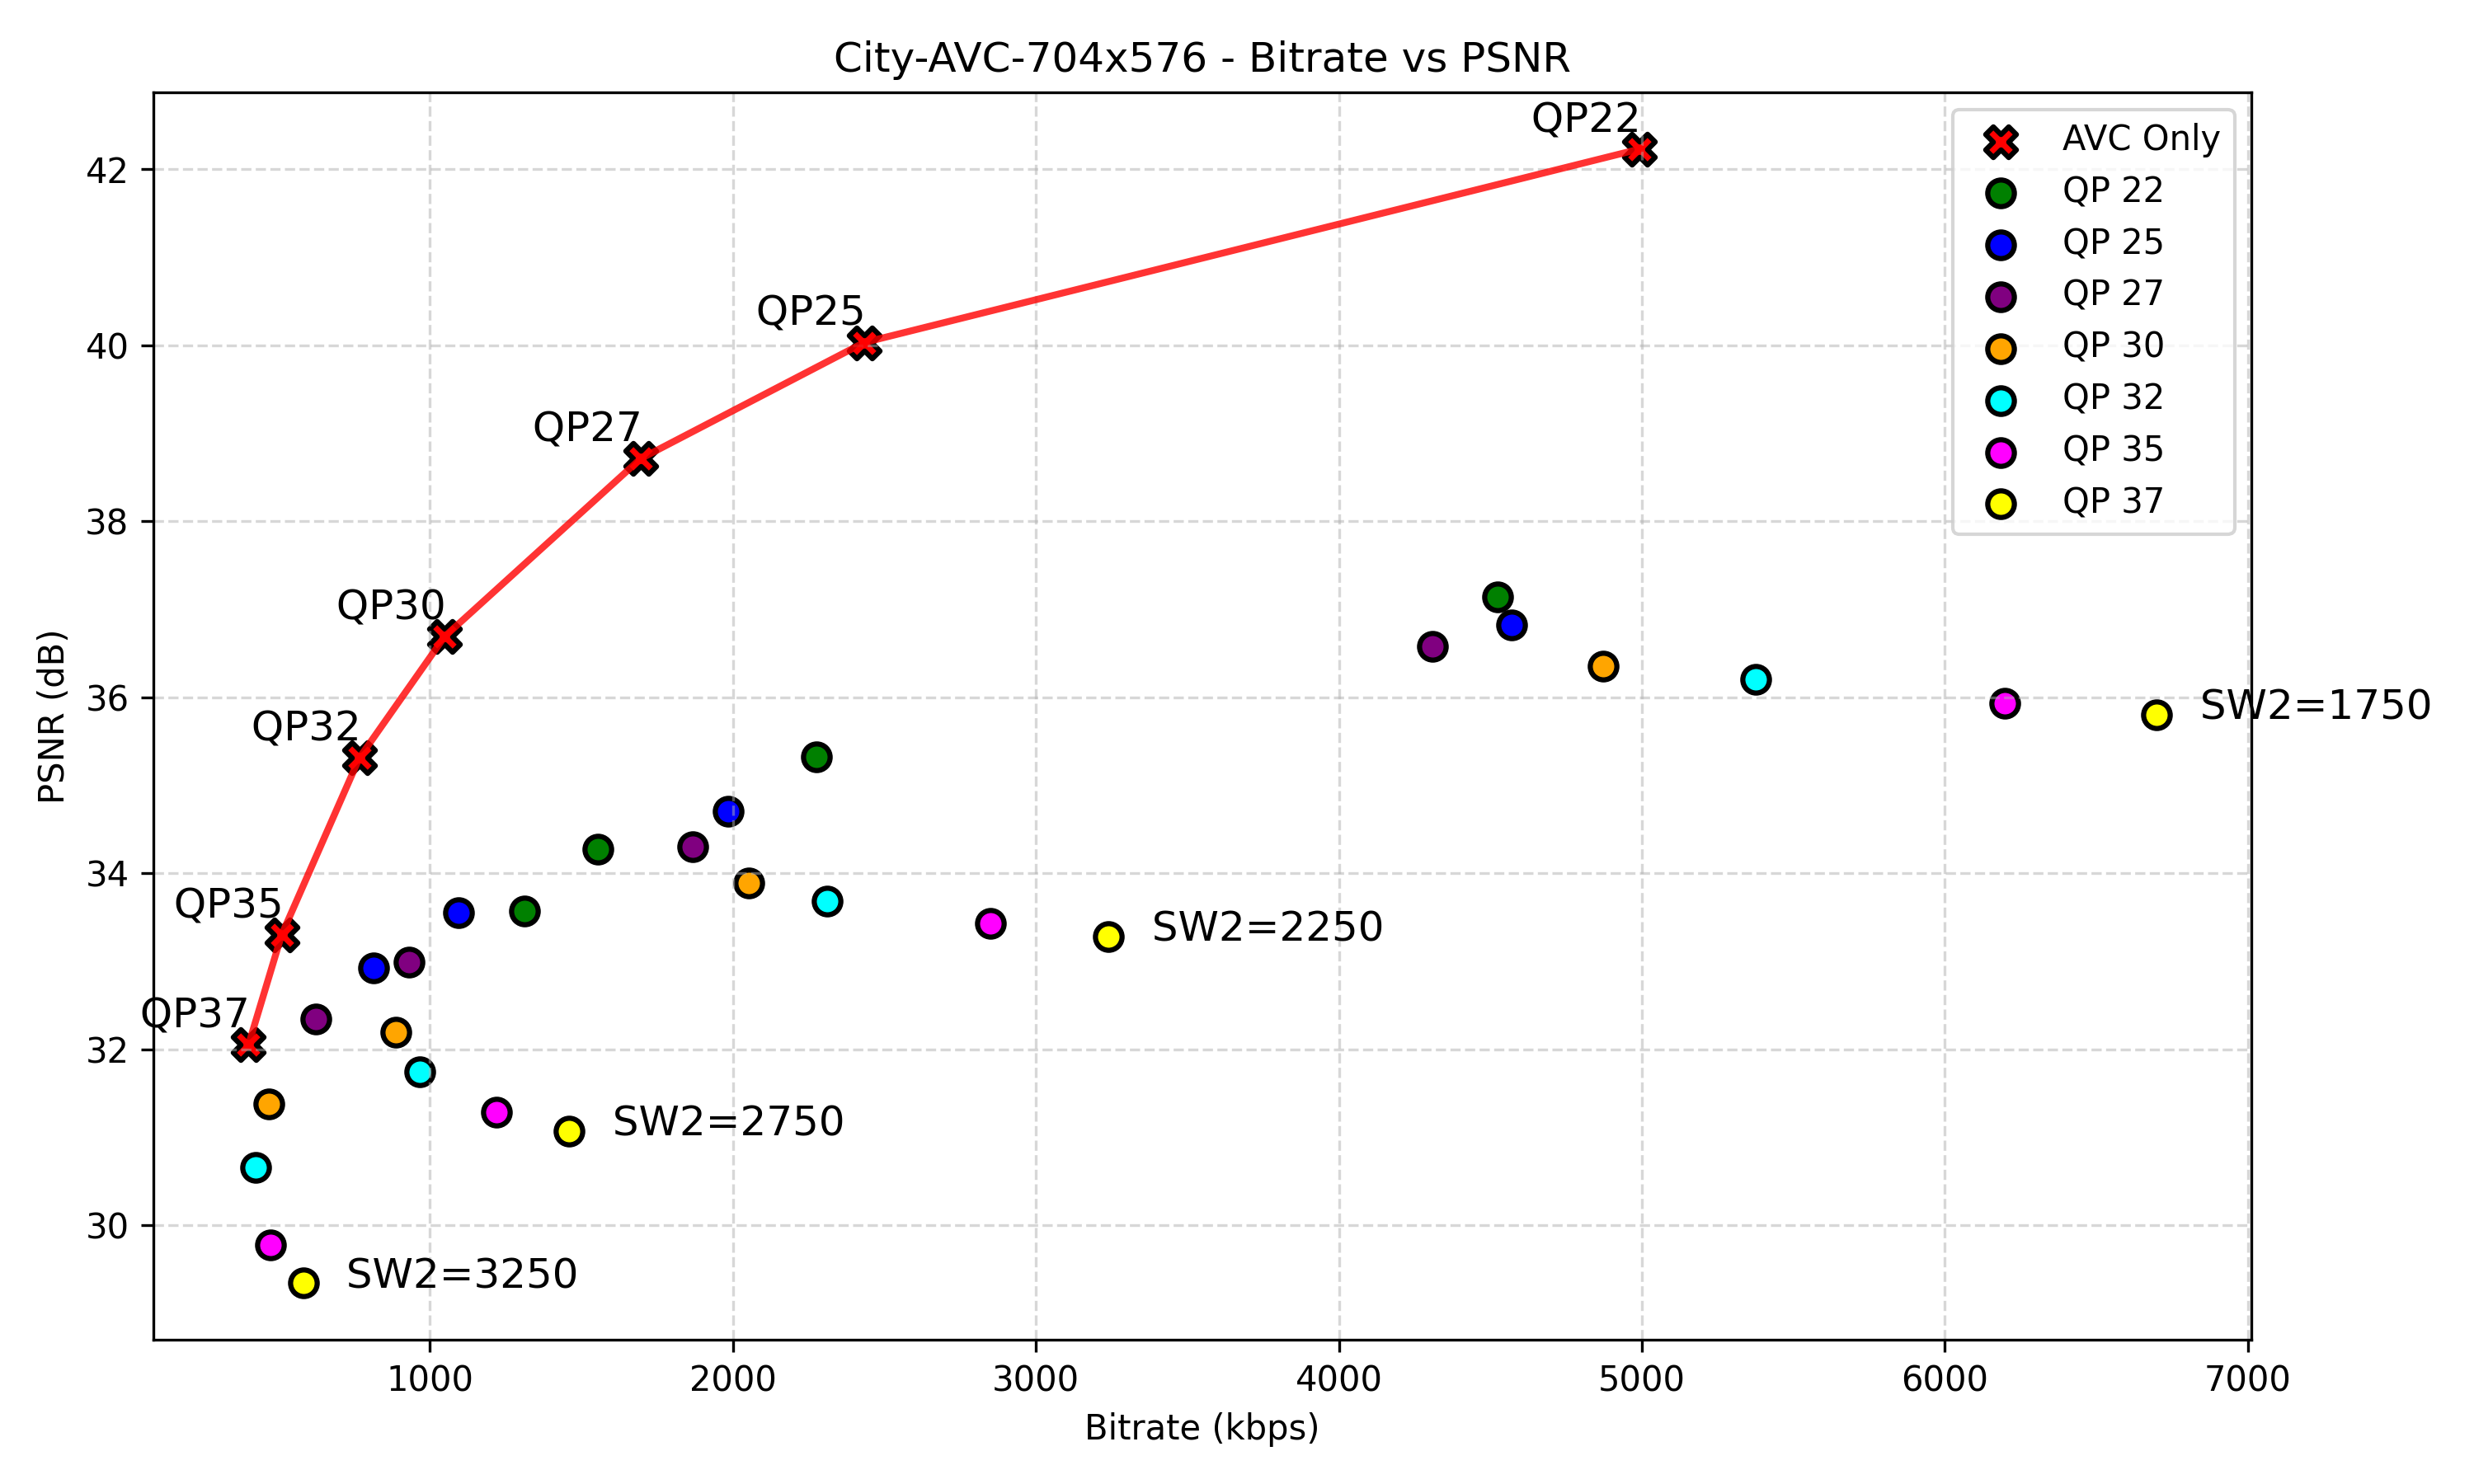
\includegraphics[width=1.0\textwidth]{img/City-AVC.png}
    \caption{Resultados para "City"\ em \acrshort{AVC}. \cite{xiph}}
    \label{fig:City}
\end{figure}

Na sequência City, o \acrshort{LCEVC} não demonstrou uma performance satisfatória. Mais 
uma sequência com uma resolução menor que 1080p que o \acrshort{LCEVC} não obtêm um resultado
ótimo. Neste caso, o \acrshort{LCEVC} não demonstrou um benefício em seu uso, no caso da relação
qualidade-tamanho, e não obteve um \acrshort{PSNR} superior à curva de referência em nenhum ponto.

\newpage
\subsection{vc-globo-05}

\begin{figure}[h]
    \centering
    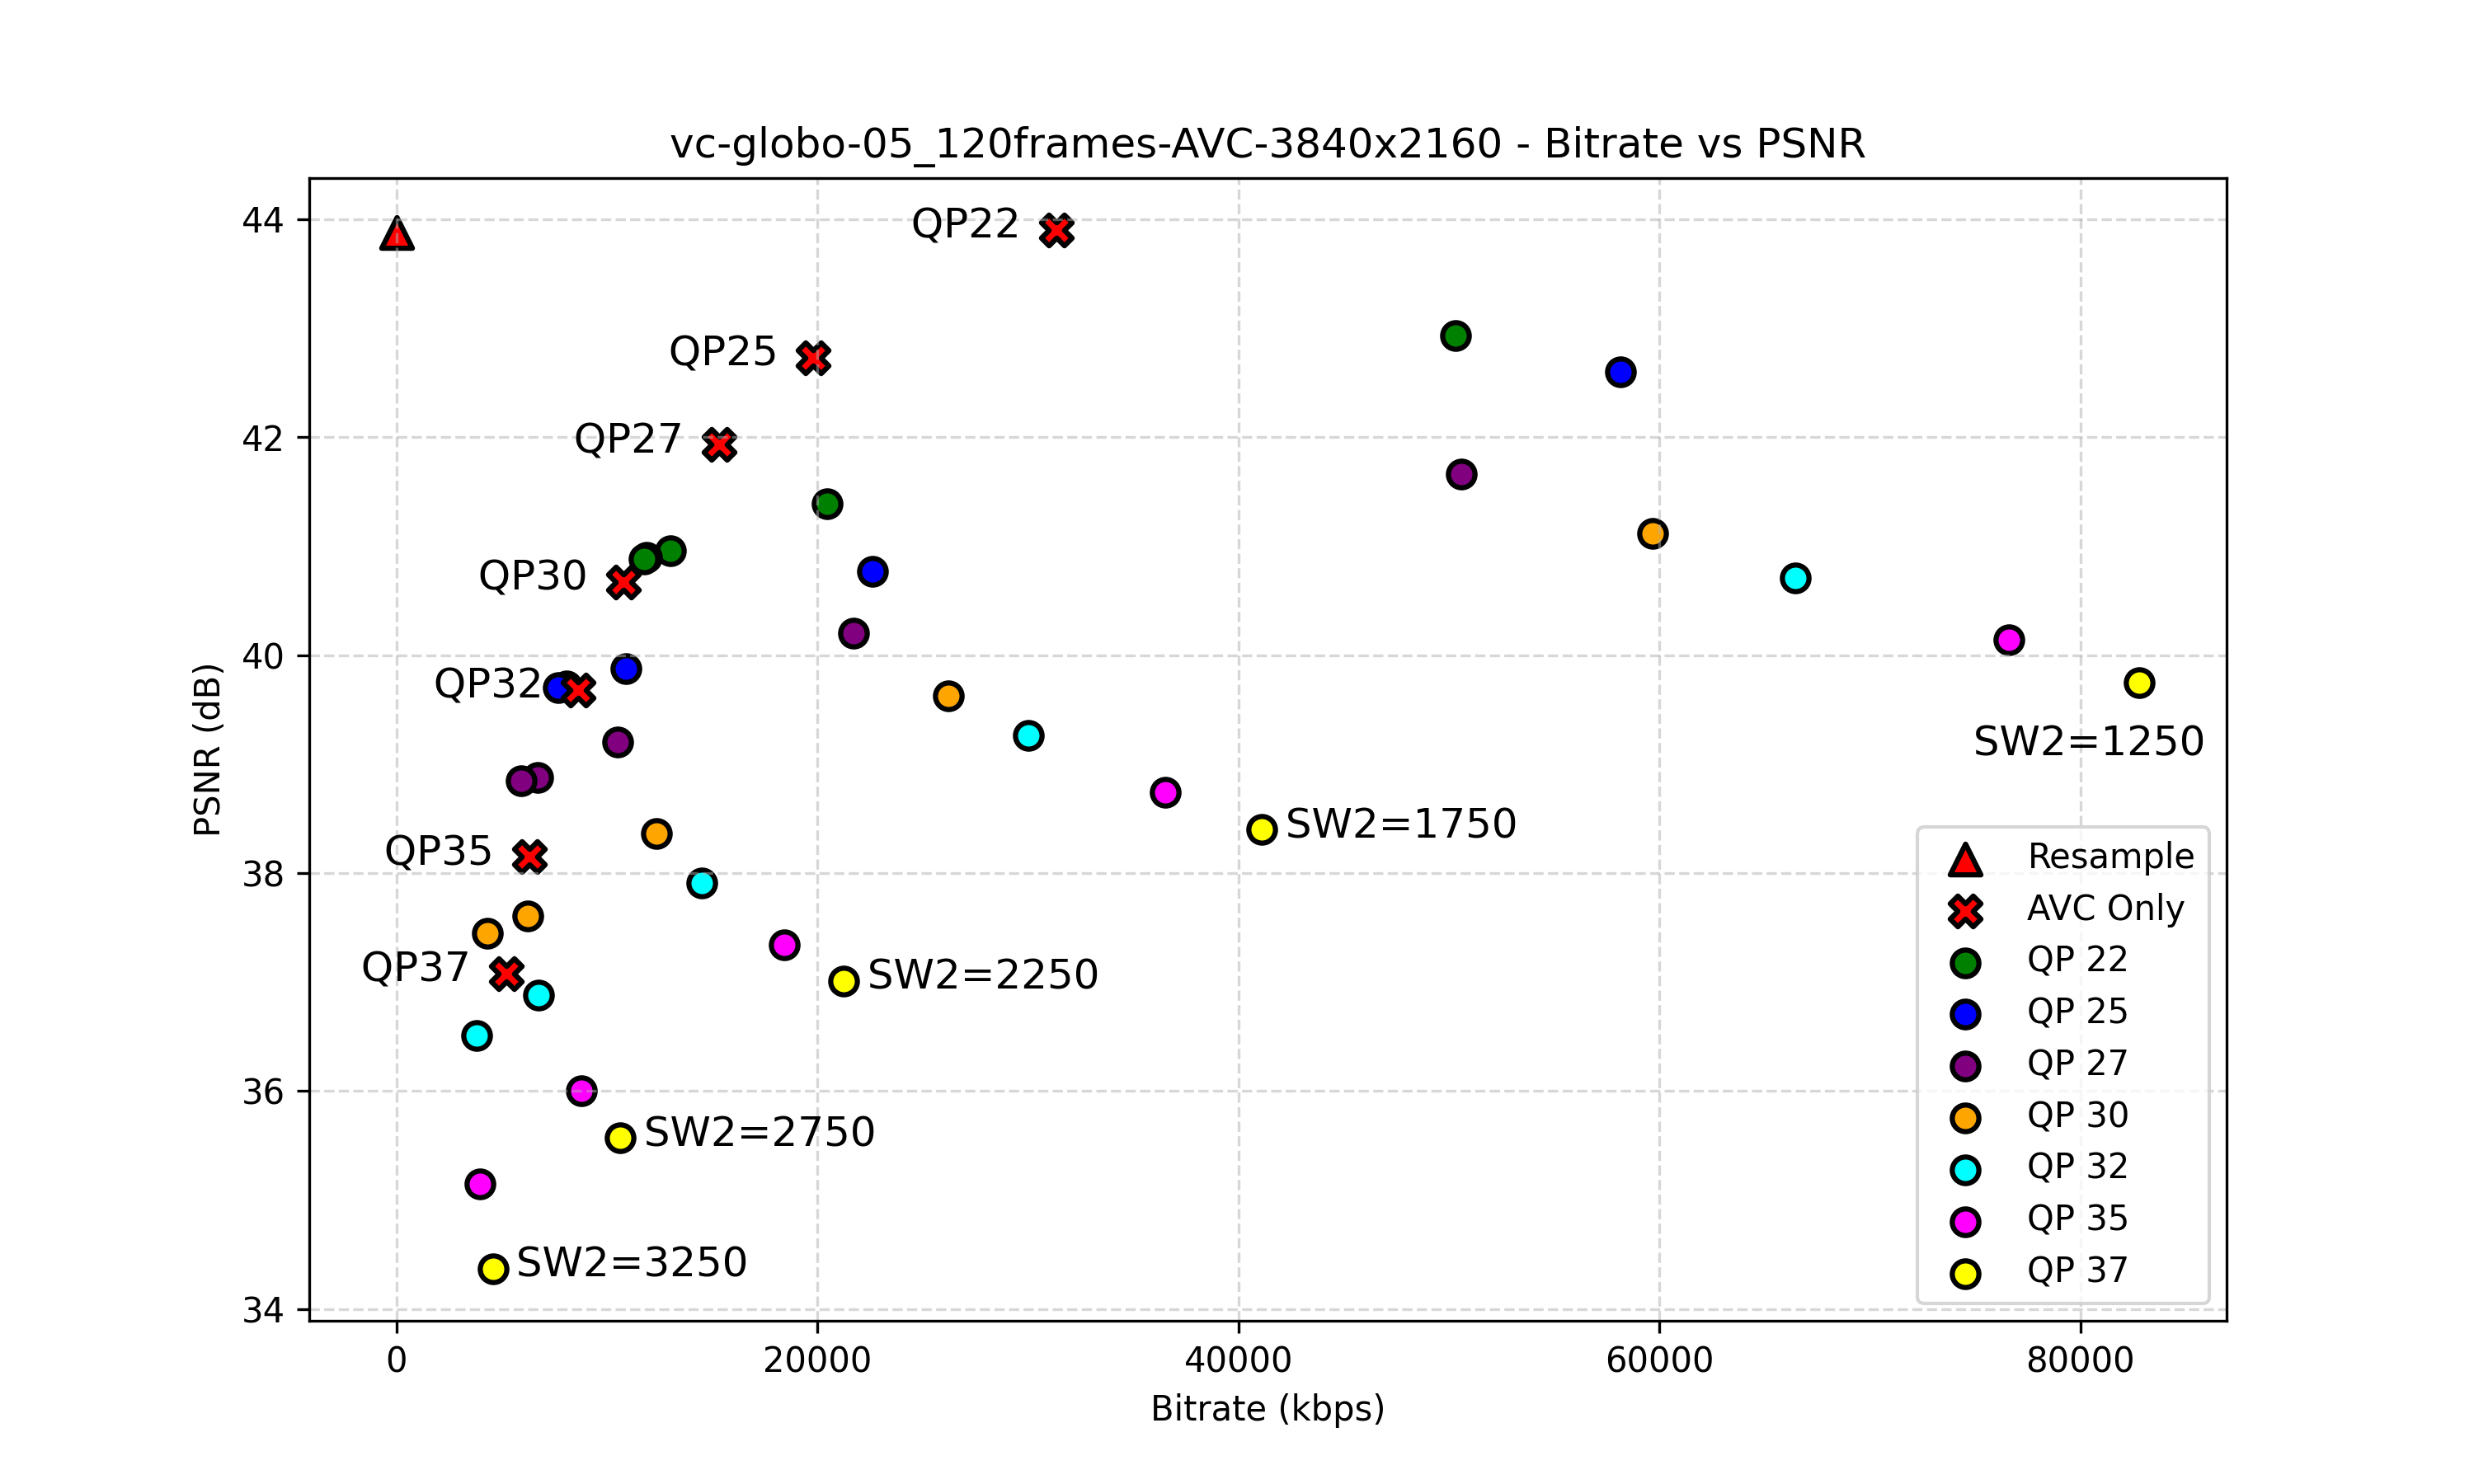
\includegraphics[width=1.0\textwidth]{img/vc-globo-05_120frames-AVC.png}
    \caption{Resultados para "vc-globo-05"\ em \acrshort{AVC}. \cite{globo_video_uhd}}
    \label{fig:vc-globo-05}
\end{figure}

Para esta sequência,o \acrshort{LCEVC} conseguiu obter resultados satisfatório acima da curva
de referência do \acrshort{AVC}. Os QPs que se destacaram para o \acrshort{LCEVC} foram: 30,
27 e 25. Os resultados obtidos para QP 22 foram muito próximos da curva, onde mesmo não estando
acima, ainda representa um valor satisfatório, por manter a qualidade que o \acrshort{AVC} obteve.
Os resultados favoráveis ao \acrshort{LCEVC} estão abaixo.

\begin{table}[h]
    \centering
    \begin{tabular}{|c|c|c|c|}
        \hline
        \textbf{QP} & \textbf{Tamanho (b)} & \textbf{PSNR (dB)} & \textbf{Taxa (kbps)} \\
        \hline
        37 & 1305057 & 37.08 & 5220.23 \\
        35 & 1575423 & 38.15 & 6301.69 \\
        32 & 2158588 & 39.68 & 8634.35 \\
        30 & 2694302 & 40.67 & 10777.21 \\
        27 & 3828463 & 41.93 & 15313.85 \\
        25 & 4950018 & 42.73 & 19800.07 \\
        22 & 7836829 & 43.90 & 31347.32 \\
        \hline
    \end{tabular}
    \caption{Resultados para vc-globo-05 em AVC.}
    \label{tab:vc-globo-05-avc}
\end{table}

\begin{table}[h]
    \centering
    \label{tab:vc-globo-05-avc-lcevc}
    \begin{tabular}{|c|c|c|c|c|c|c|c|}
        \hline
        \textbf{SW2} & \textbf{QP} & \textbf{Tamanho (b)} & \textbf{Proporção} & \textbf{PSNR (dB)} & \textbf{Taxa (kbps)} & \textbf{Superou} \\
        \hline
            3250 & 30 & 1079936 & 8.22\% & 37.45 & 4319.74 & AVC QP37 \\
            3250 & 27 & 1480606 & 1.49\% & 38.85 & 5922.42 & AVC QP35 \\
            2750 & 27 & 1681499 & 13.26\% & 38.88 & 6726.00 & AVC QP35 \\
            3250 & 25 & 1924885 & 0.68\% & 39.70 & 7699.54 & AVC QP32 \\
            2750 & 25 & 2021470 & 5.43\% & 39.72 & 8085.88 & AVC QP32 \\
        \hline
    \end{tabular}
    \caption{Resultados favoráveis do LCEVC para vc-globo-05 em AVC.}
\end{table}

\newpage
\subsection{vc-lcevc-01}

\begin{figure}[h]
    \centering
    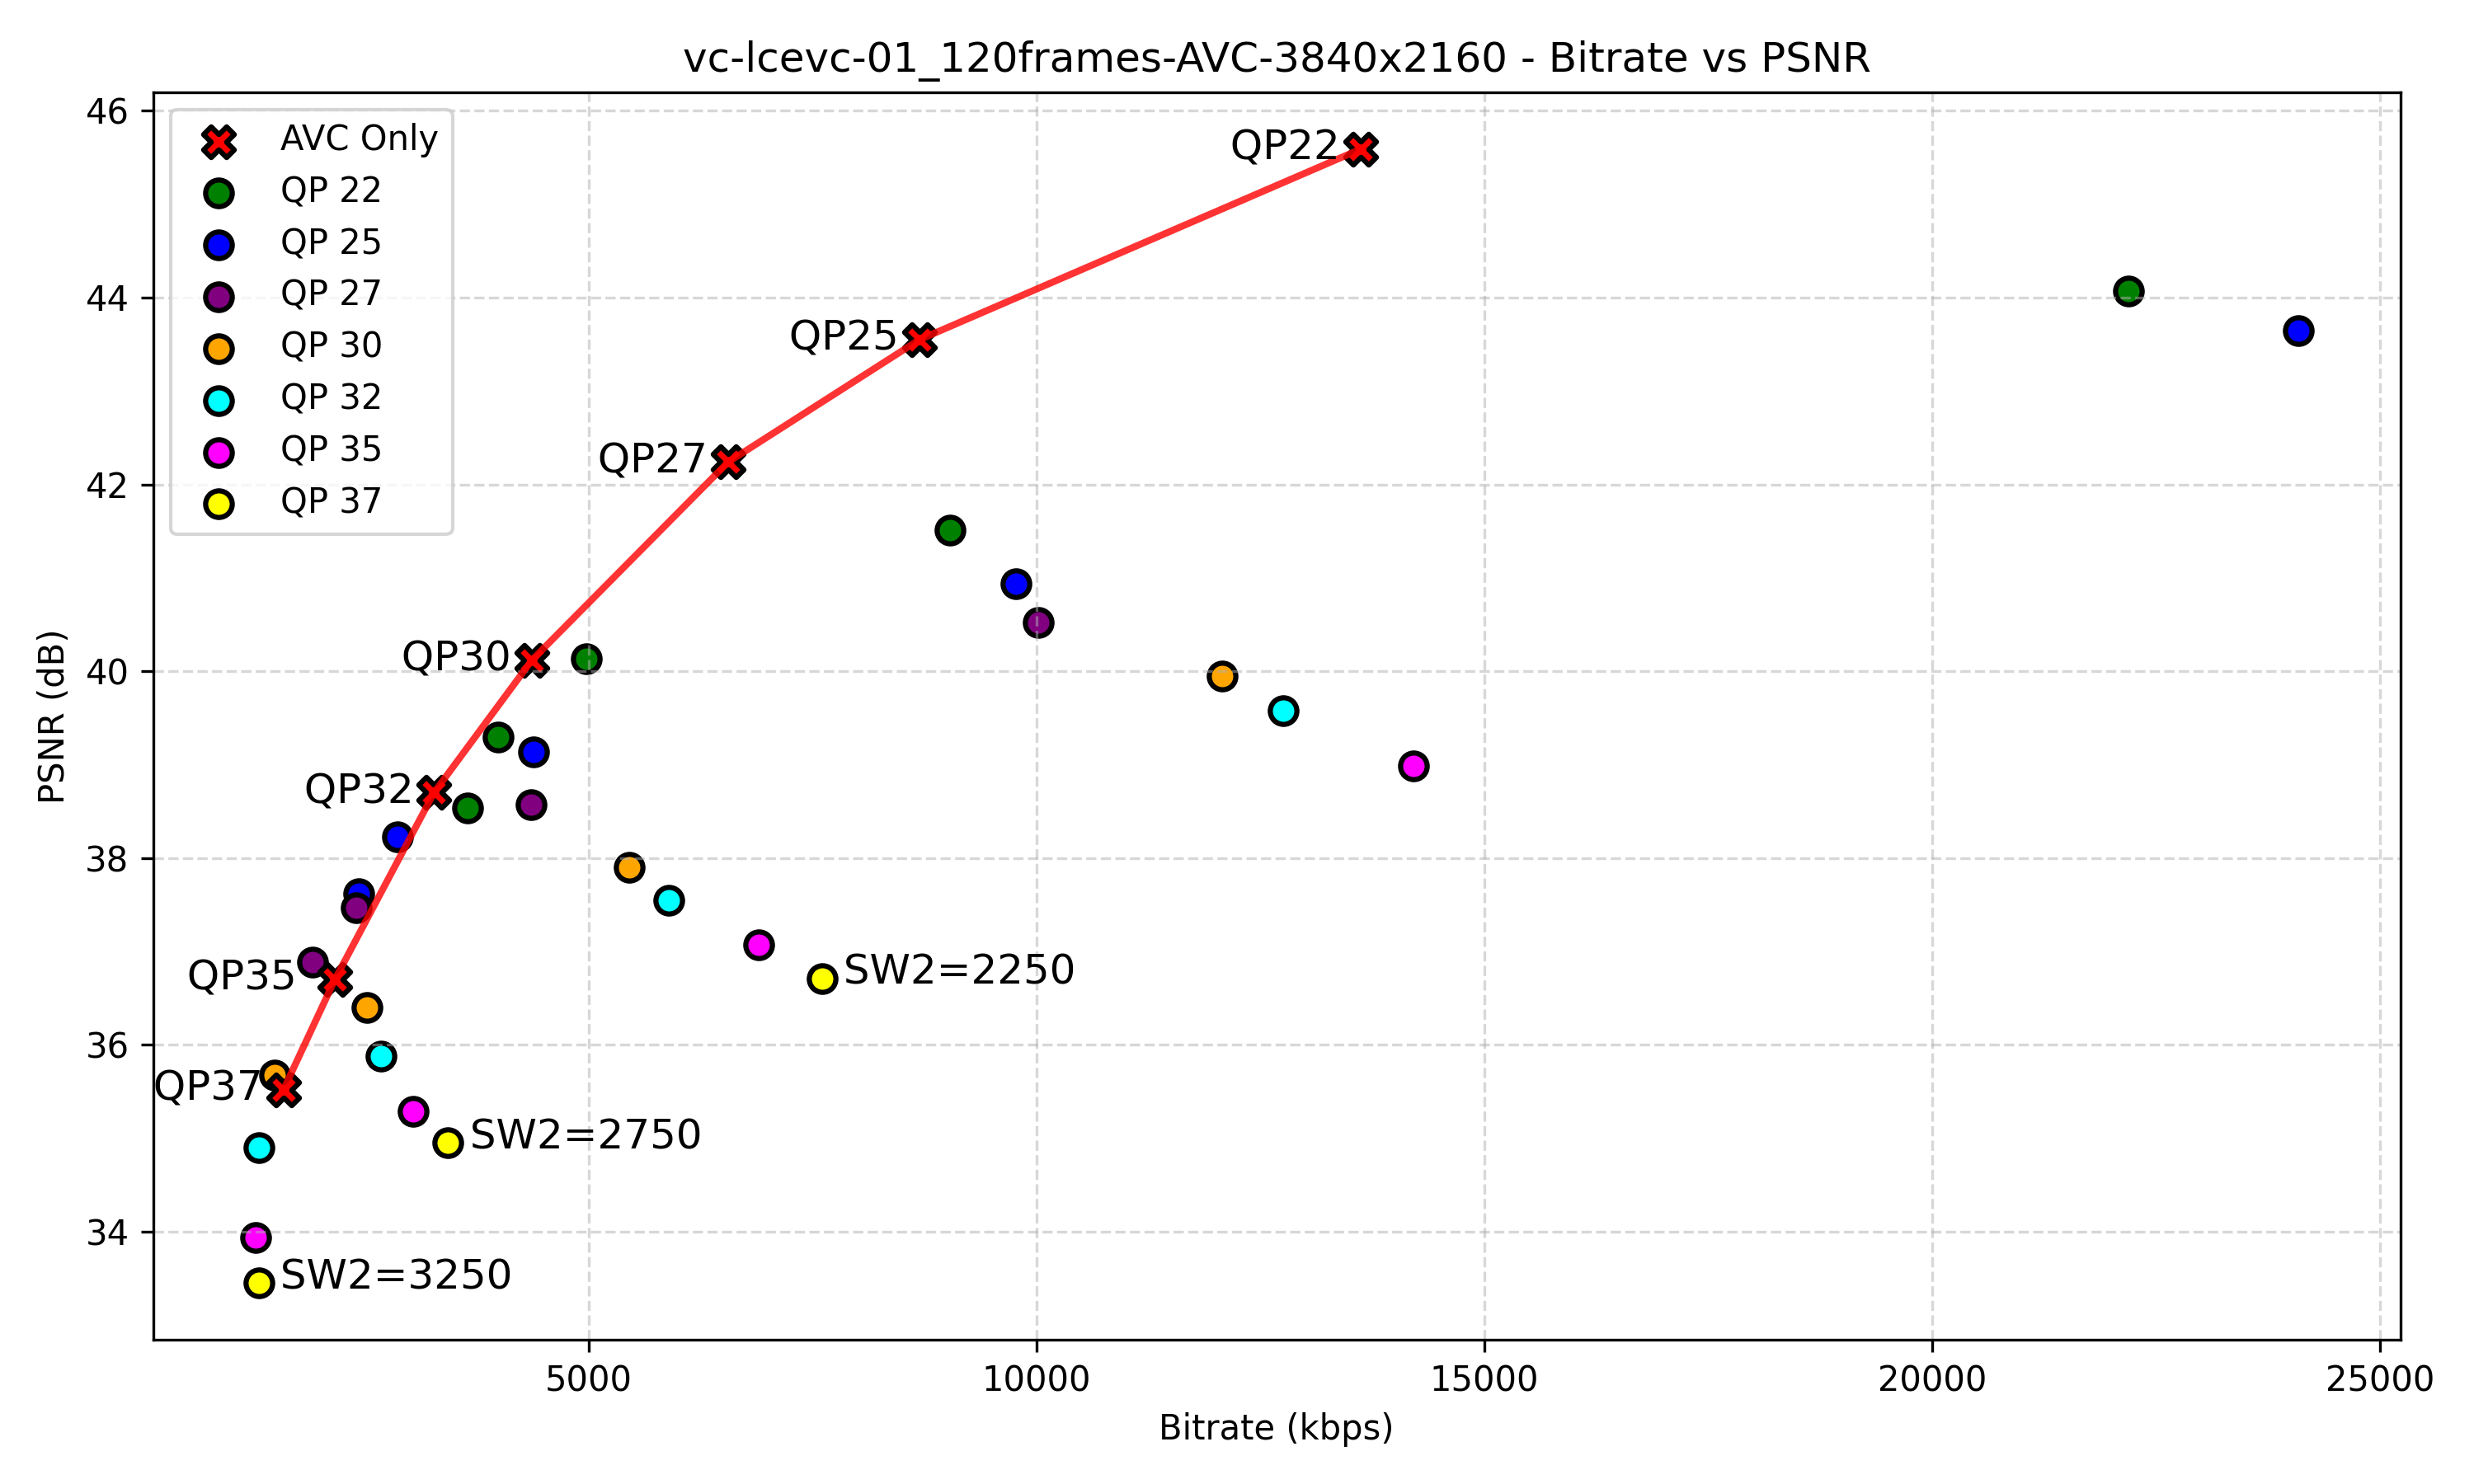
\includegraphics[width=1.0\textwidth]{img/vc-lcevc-01_120frames-AVC.png}
    \caption{Resultados para "vc-lcevc-01"\ em \acrshort{AVC}.}
    \label{fig:vc-lcevc-01}
\end{figure}

Nesta sequência, o \acrshort{LCEVC} conseguiu resultados relevantes para QP igual
a 30, 27 e 25. Para o QP de 22, ele não conseguiu alcançar a curva do \acrshort{AVC}.
Os resultados favoráveis ficaram bem próximos da curva do \acrshort{AVC}. Os 
resultados são apresentados a seguir.

\begin{table}[h]
    \centering
    \begin{tabular}{|c|c|c|c|}
        \hline
        \textbf{QP} & \textbf{Tamanho (b)} & \textbf{PSNR (dB)} & \textbf{Taxa (kbps)} \\
        \hline
        37 & 398114 & 35.52 & 1592.46 \\
        35 & 541605 & 36.70 & 2166.42 \\
        32 & 818304 & 38.70 & 3273.22 \\
        30 & 1091870 & 40.12 & 4367.48 \\
        27 & 1639723 & 42.24 & 6558.89 \\
        25 & 2173840 & 43.55 & 8695.36 \\
        22 & 3405589 & 45.59 & 13622.36 \\
        \hline
    \end{tabular}
    \caption{Resultados para vc-lcevc-01 em AVC.}
    \label{tab:vc-lcevc-01-avc}
\end{table}

\begin{table}[h]
    \centering
    \label{tab:vc-lcevc-01-avc-lcevc}
    \begin{tabular}{|c|c|c|c|c|c|c|c|}
        \hline
        \textbf{SW2} & \textbf{QP} & \textbf{Tamanho (b)} & \textbf{Proporção} & \textbf{PSNR (dB)} & \textbf{Taxa (kbps)} & \textbf{Superou} \\
        \hline
        3250 & 30 & 373846 & 28.13\% & 35.68 & 1495.38 & AVC QP37 \\
        3250 & 27 & 480407 & 17.20\% & 36.89 & 1921.63 & AVC QP35 \\
        2750 & 27 & 600914 & 33.80\% & 37.47 & 2403.66 & AVC QP35 \\
        3250 & 25 & 608435 & 13.11\% & 37.62 & 2433.74 & AVC QP35 \\
        2750 & 25 & 715498 & 26.11\% & 38.23 & 2861.99 & AVC QP35 \\
        \hline
    \end{tabular}
    \caption{Resultados favoráveis do LCEVC para vc-lcevc-01 em AVC.}
\end{table}

\newpage
\subsection{vc-philips-01}

\begin{figure}[h]
    \centering
    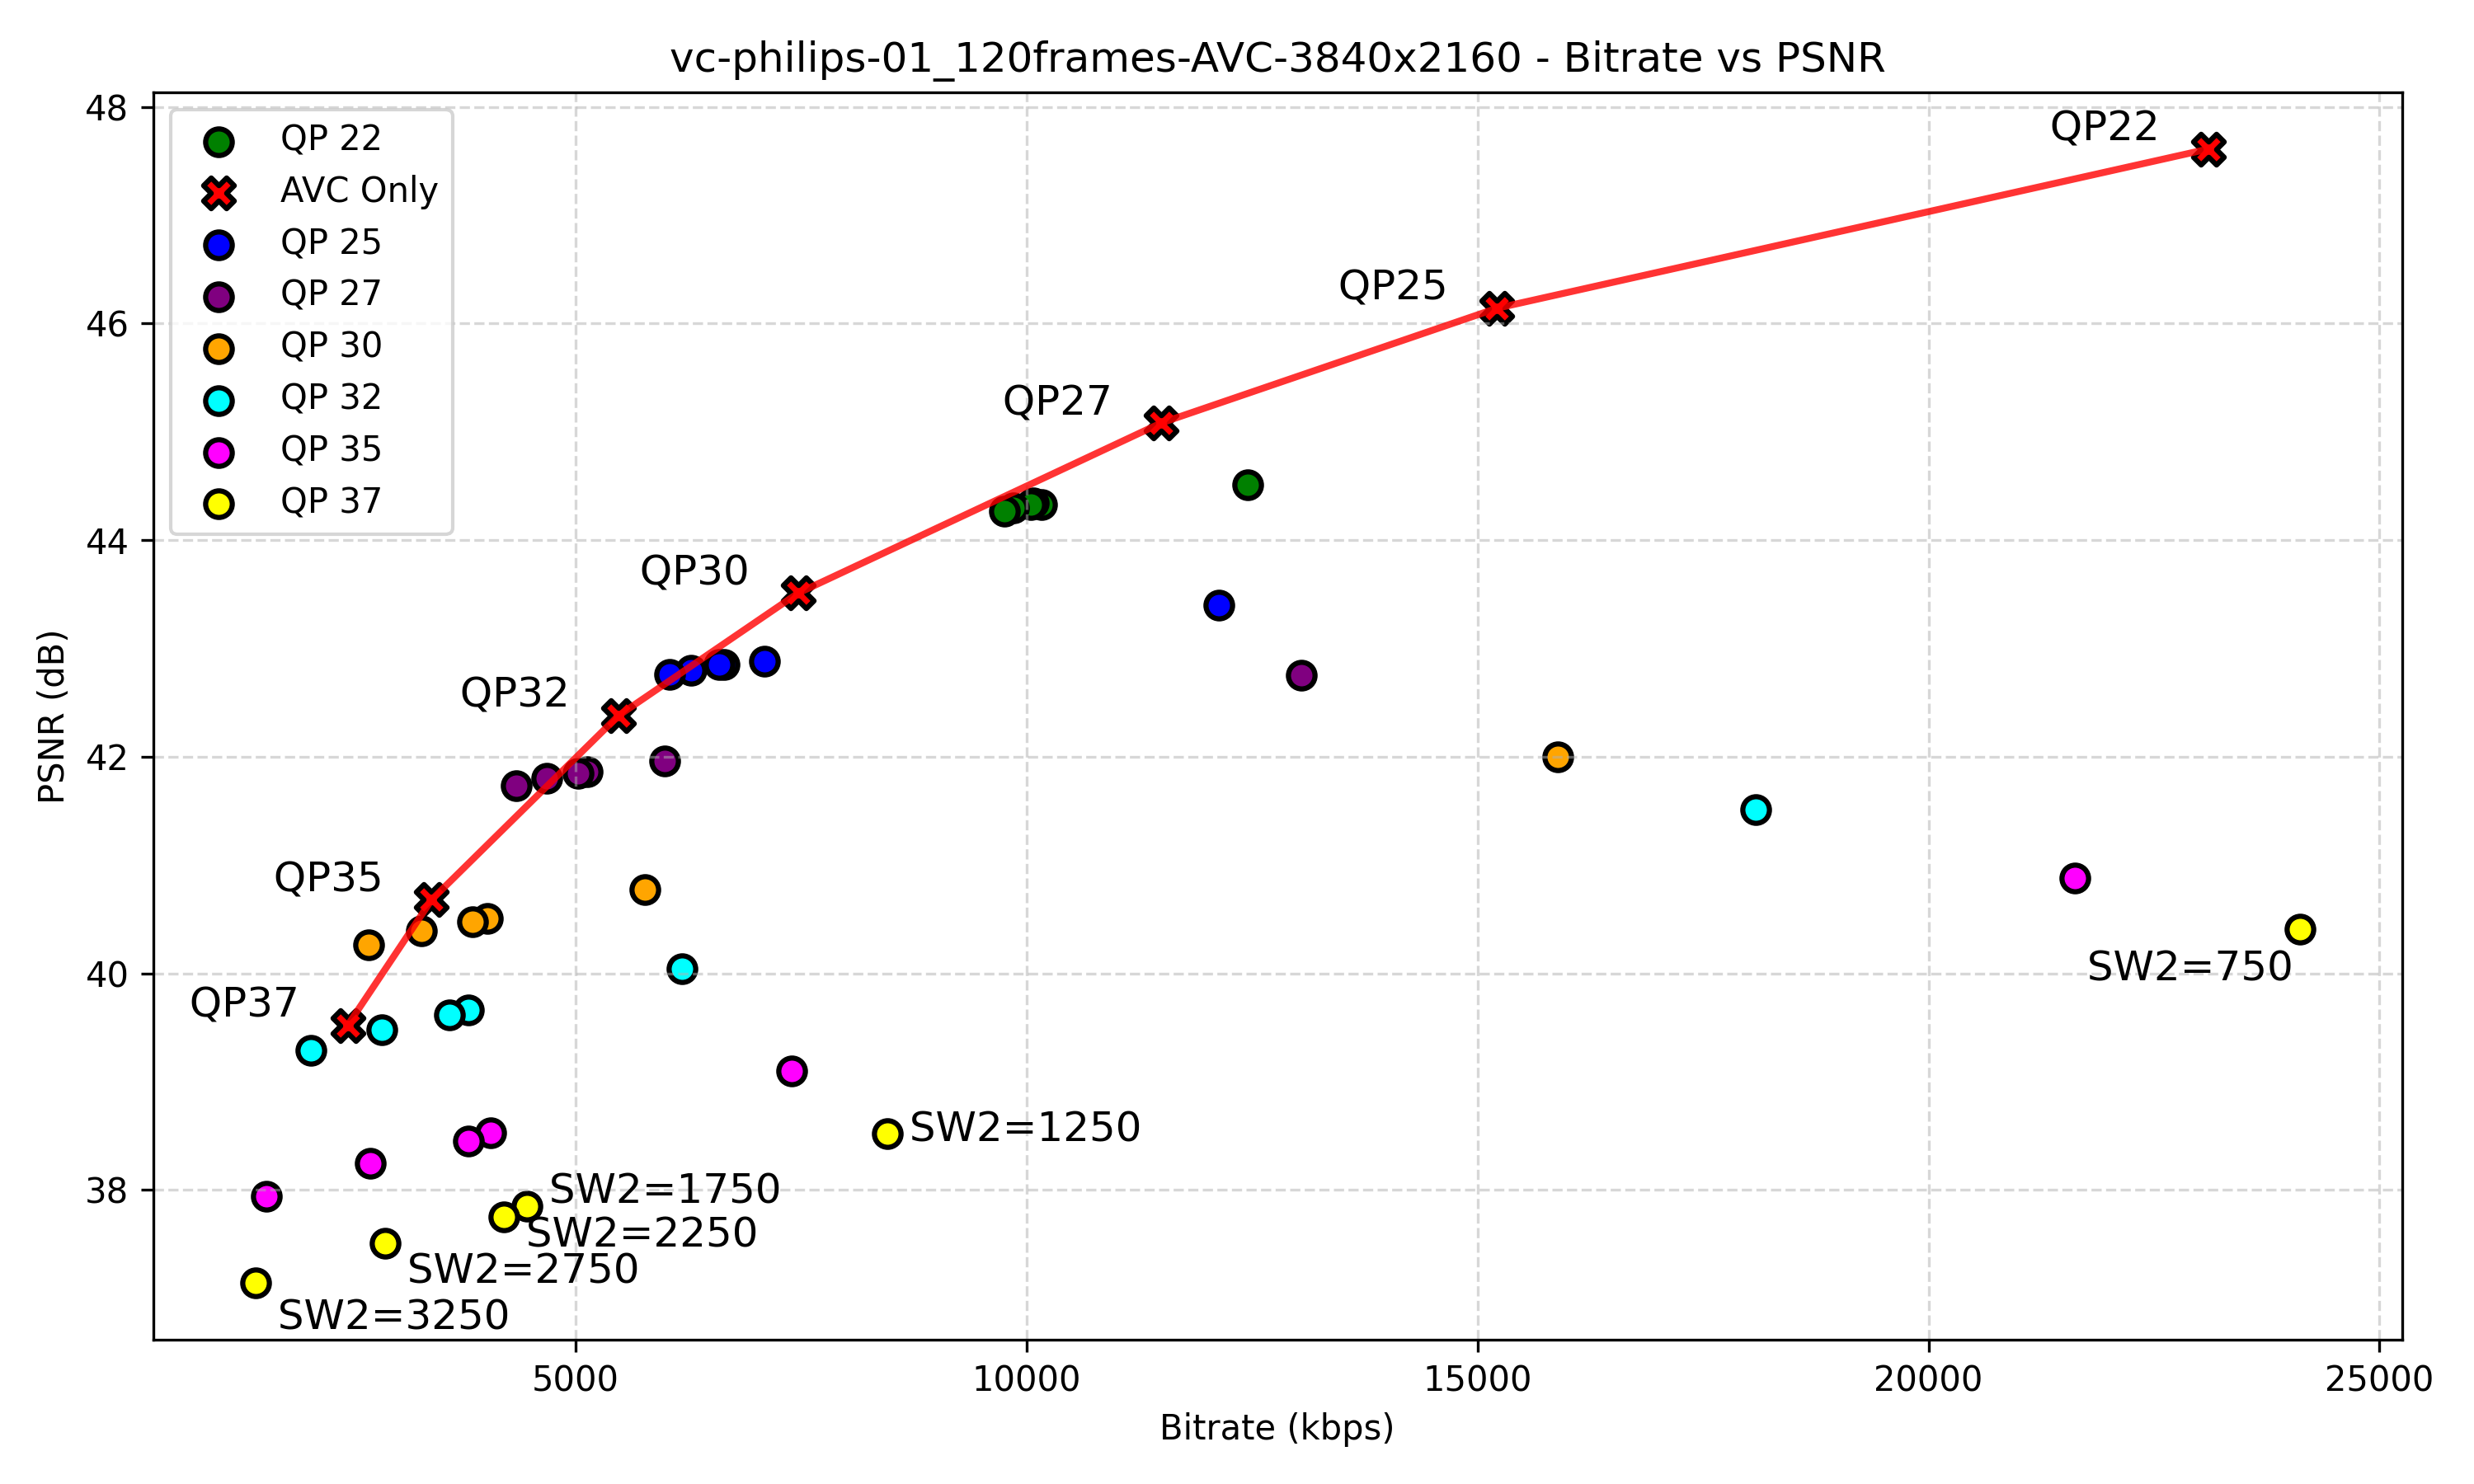
\includegraphics[width=0.79\textwidth]{img/vc-philips-01_120frames-AVC.png}
    \caption{Resultados para "vc-philips-01"\ em \acrshort{AVC}.}
    \label{fig:vc-philips-01}
\end{figure}

\newpage
Aqui, o \acrshort{LCEVC} obteve alguns resultados acima da curva do \acrshort{AVC},
mostrando obter resultados superiores ao \acrshort{AVC} puro. Os QPs que se destacaram
neste resultado foram 30, 27, e 25. Estes valores conseguiram resultados acima da curva.

\begin{table}[h]
    \centering
    \begin{tabular}{|c|c|c|c|}
        \hline
        \textbf{QP} & \textbf{Tamanho (b)} & \textbf{PSNR (dB)} & \textbf{Taxa (kbps)} \\
        \hline
        37 & 617900 & 39.52 & 2471.60 \\
        35 & 850687 & 40.68 & 3402.75 \\
        32 & 1368899 & 42.38 & 5475.60 \\
        30 & 1866486 & 43.51 & 7465.94 \\
        27 & 2872324 & 45.08 & 11489.30 \\
        25 & 3803303 & 46.14 & 15213.21 \\
        22 & 5775373 & 47.61 & 23101.49 \\
        \hline
    \end{tabular}
    \caption{Resultados para vc-philips-01 em AVC.}
    \label{tab:vc-philips-01-avc}
\end{table}

\begin{table}[h]
    \centering
    \label{tab:vc-philips-01-avc-philips}
    \begin{tabular}{|c|c|c|c|c|c|c|c|}
        \hline
        \textbf{SW2} & \textbf{QP} & \textbf{Tamanho (b)} & \textbf{Proporção} & \textbf{PSNR (dB)} & \textbf{Taxa (kbps)} & \textbf{Superou} \\
        \hline
        3250 & 30 & 54458 & 8.05\% & 40.26 & 2704.88 & AVC QP37 \\
        3250 & 27 & 20276 & 1.87\% & 41.73 & 4338.48 & AVC QP37 \\
        2750 & 27 & 104990 & 8.98\% & 41.80 & 4677.34 & AVC QP35 \\
        3250 & 25 & 9350 & 0.62\% & 42.76 & 6043.10 & AVC QP32-30 \\
        \hline
    \end{tabular}
    \caption{Resultados favoráveis do LCEVC para vc-philips-01 em AVC.}
\end{table}

\newpage
\subsection{vc-philips-03}

\begin{figure}[h]
    \centering
    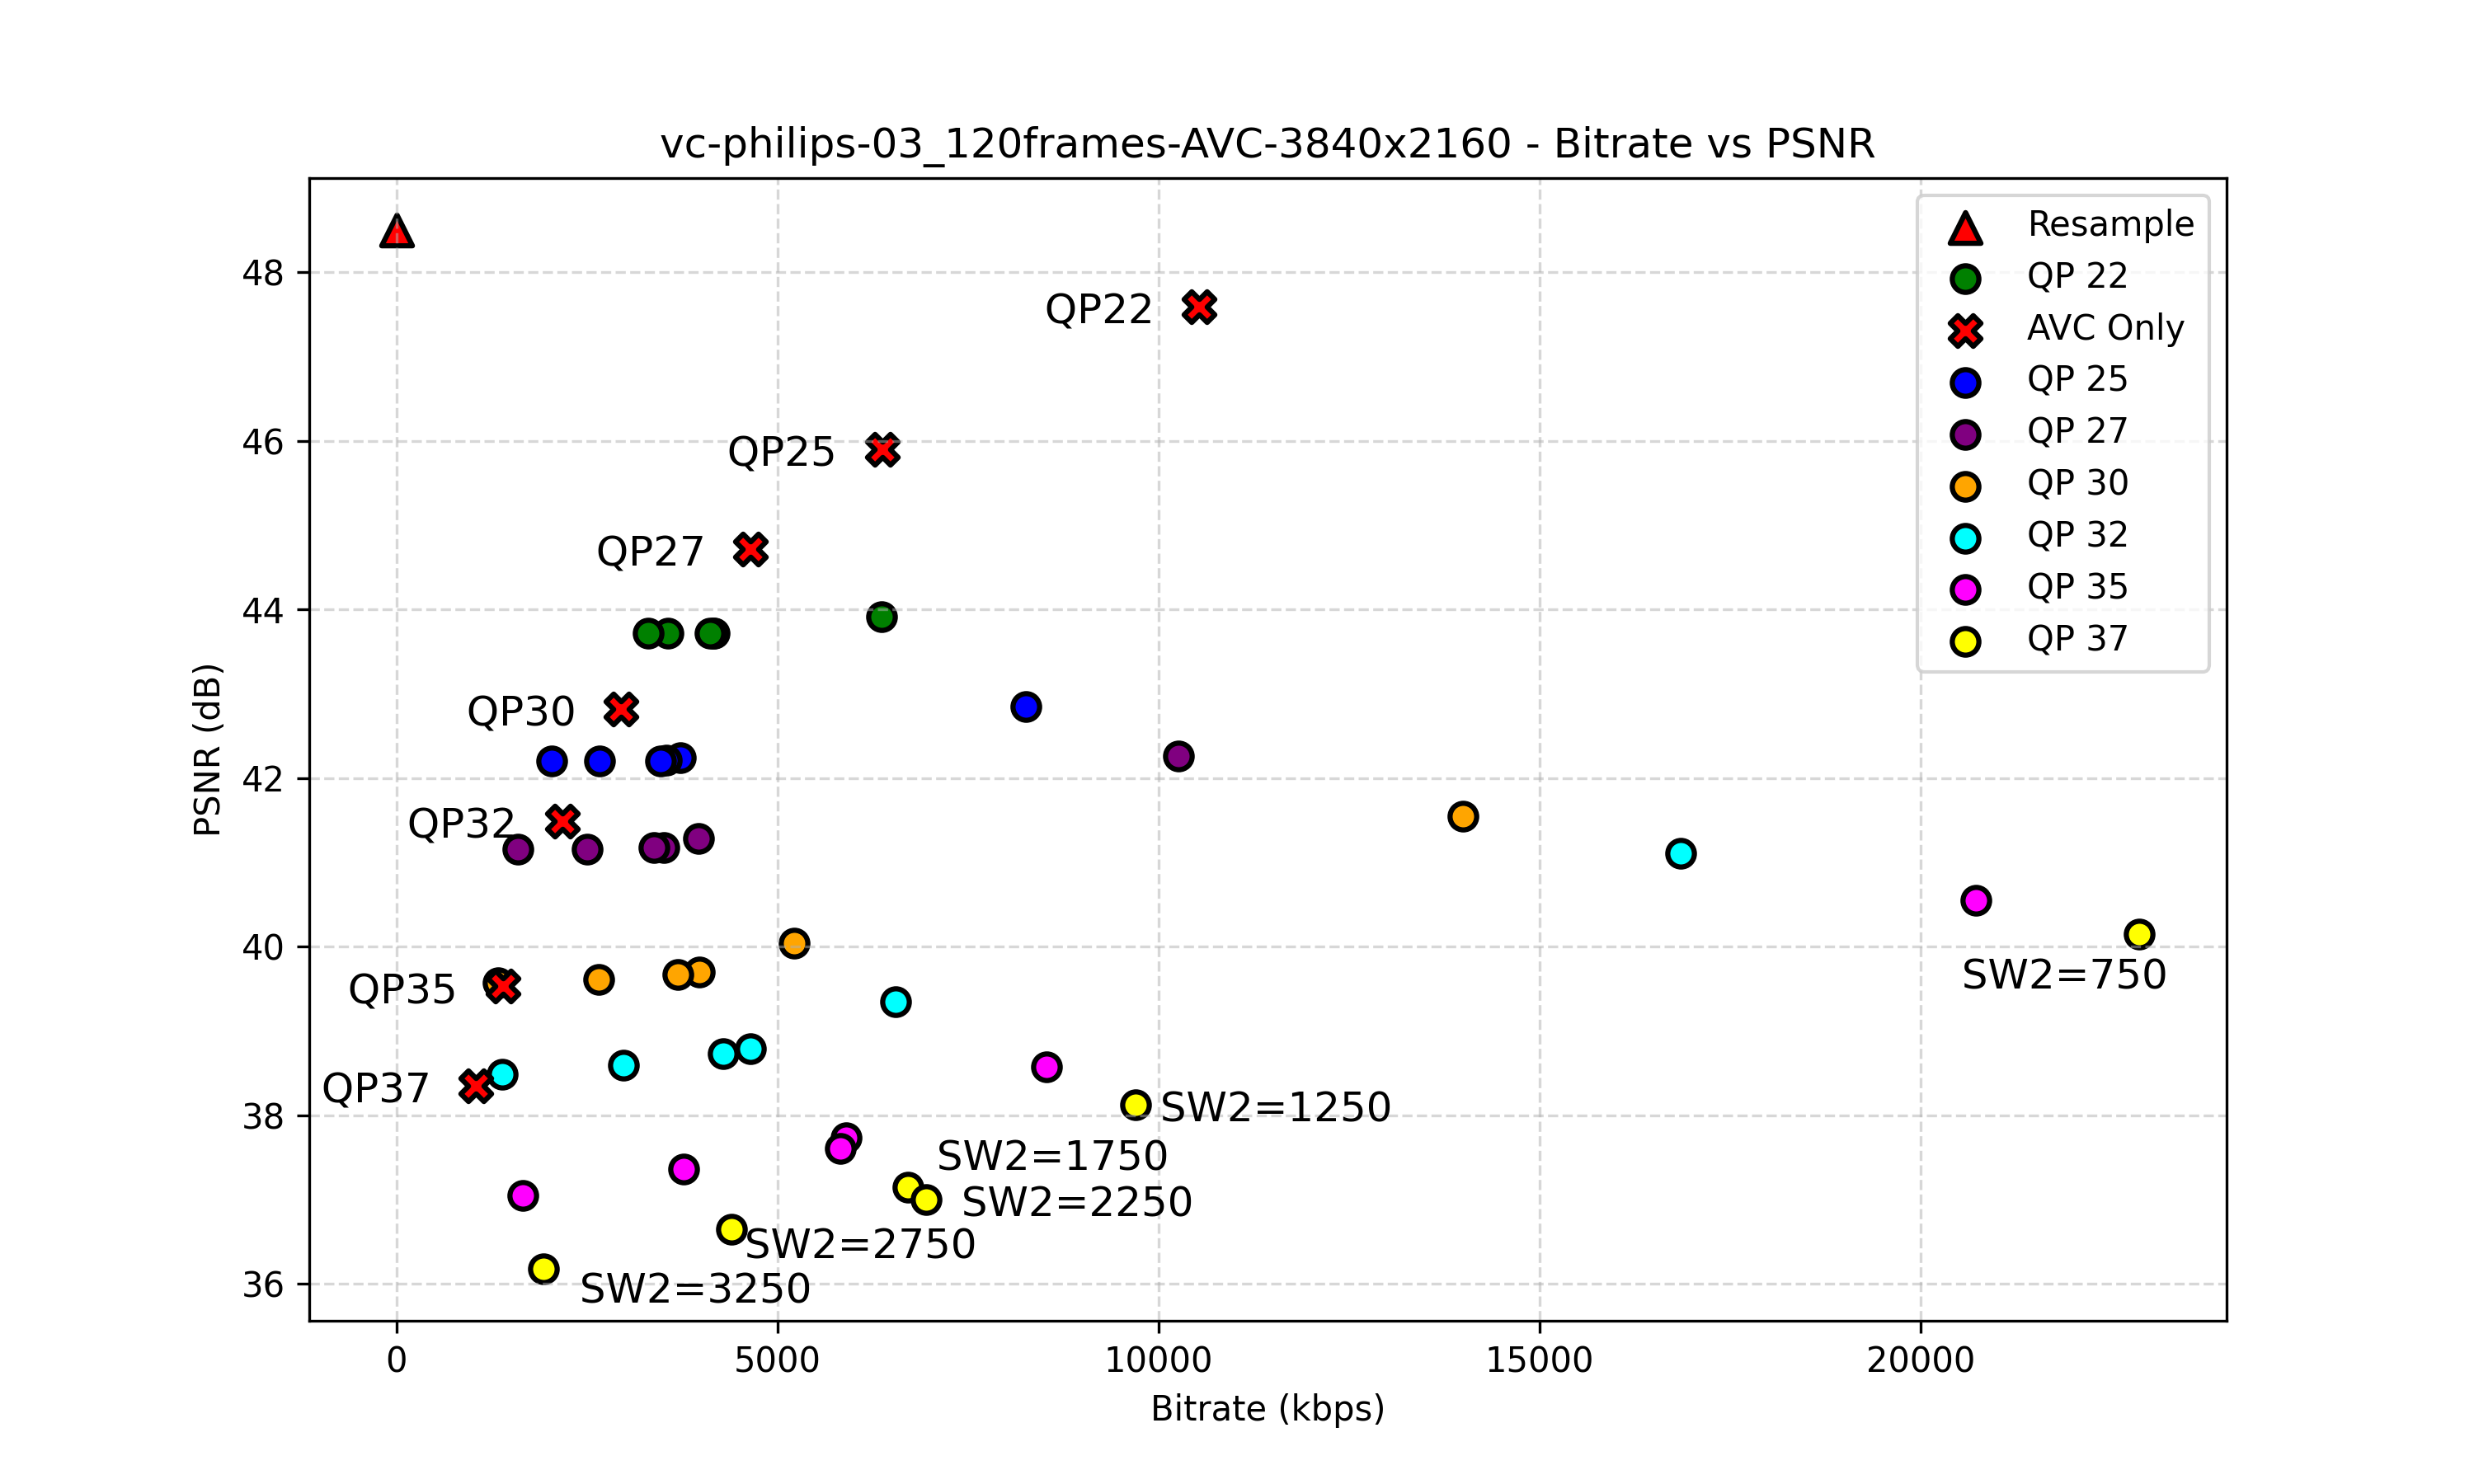
\includegraphics[width=1.0\textwidth]{img/vc-philips-03_120frames-AVC.png}
    \caption{Resultados para "vc-philips-03" em \acrshort{AVC}.}
    \label{fig:vc-philips-03}
\end{figure}

Para esta sequência, o \acrshort{LCEVC} gerou resultados melhores que o \acrshort{AVC}
puro. Novamente, os QPs menores se saíram melhor, como esperado, com destaque para os
valores de QP de 30, 27, 25 e 22.

\begin{table}[h]
    \centering
    \begin{tabular}{|c|c|c|c|}
        \hline
        \textbf{QP} & \textbf{Tamanho (b)} & \textbf{PSNR (dB)} & \textbf{Taxa (kbps)} \\
        \hline
        37 & 261857 & 38.35 & 1047.43 \\
        35 & 348522 & 39.53 & 1394.09 \\
        32 & 543963 & 41.49 & 2175.85 \\
        30 & 736459 & 42.82 & 2945.84 \\
        27 & 1161656 & 44.72 & 4646.62 \\
        25 & 1593342 & 45.90 & 6373.37 \\
        22 & 2633079 & 47.59 & 10532.32 \\
        \hline
    \end{tabular}
    \caption{Resultados para vc-philips-03 em AVC.}
    \label{tab:vc-philips-03-avc}
\end{table}

\newpage
\begin{table}[h]
    \centering
    \label{tab:vc-philips-03-avc-philips}
    \begin{tabular}{|c|c|c|c|c|c|c|c|}
        \hline
        \textbf{SW2} & \textbf{QP} & \textbf{Tamanho (b)} & \textbf{Proporção} & \textbf{PSNR (dB)} & \textbf{Taxa (kbps)} & \textbf{Superou} \\
        \hline
        3250 & 30 & 334155 & 31.98\% & 39.57 & 1336.62 & AVC QP35 \\
        3250 & 27 & 399297 & 9.08\% & 41.16 & 1597.19 & AVC QP35 \\
        3250 & 25 & 509493 & 2.68\% & 42.20 & 2037.97 & AVC QP32 \\
        3250 & 22 & 826826 & 0.61\% & 43.72 & 3307.30 & AVC QP30 \\
        2750 & 22 & 890314 & 7.70\% & 43.72 & 3561.26 & AVC QP30 \\
        \hline
    \end{tabular}
    \caption{Resultados favoráveis do LCEVC para vc-philips-03 em AVC.}
\end{table}

\newpage
\section{VVC}

\subsection{Bosphorus}

\begin{figure}[h]
    \centering
    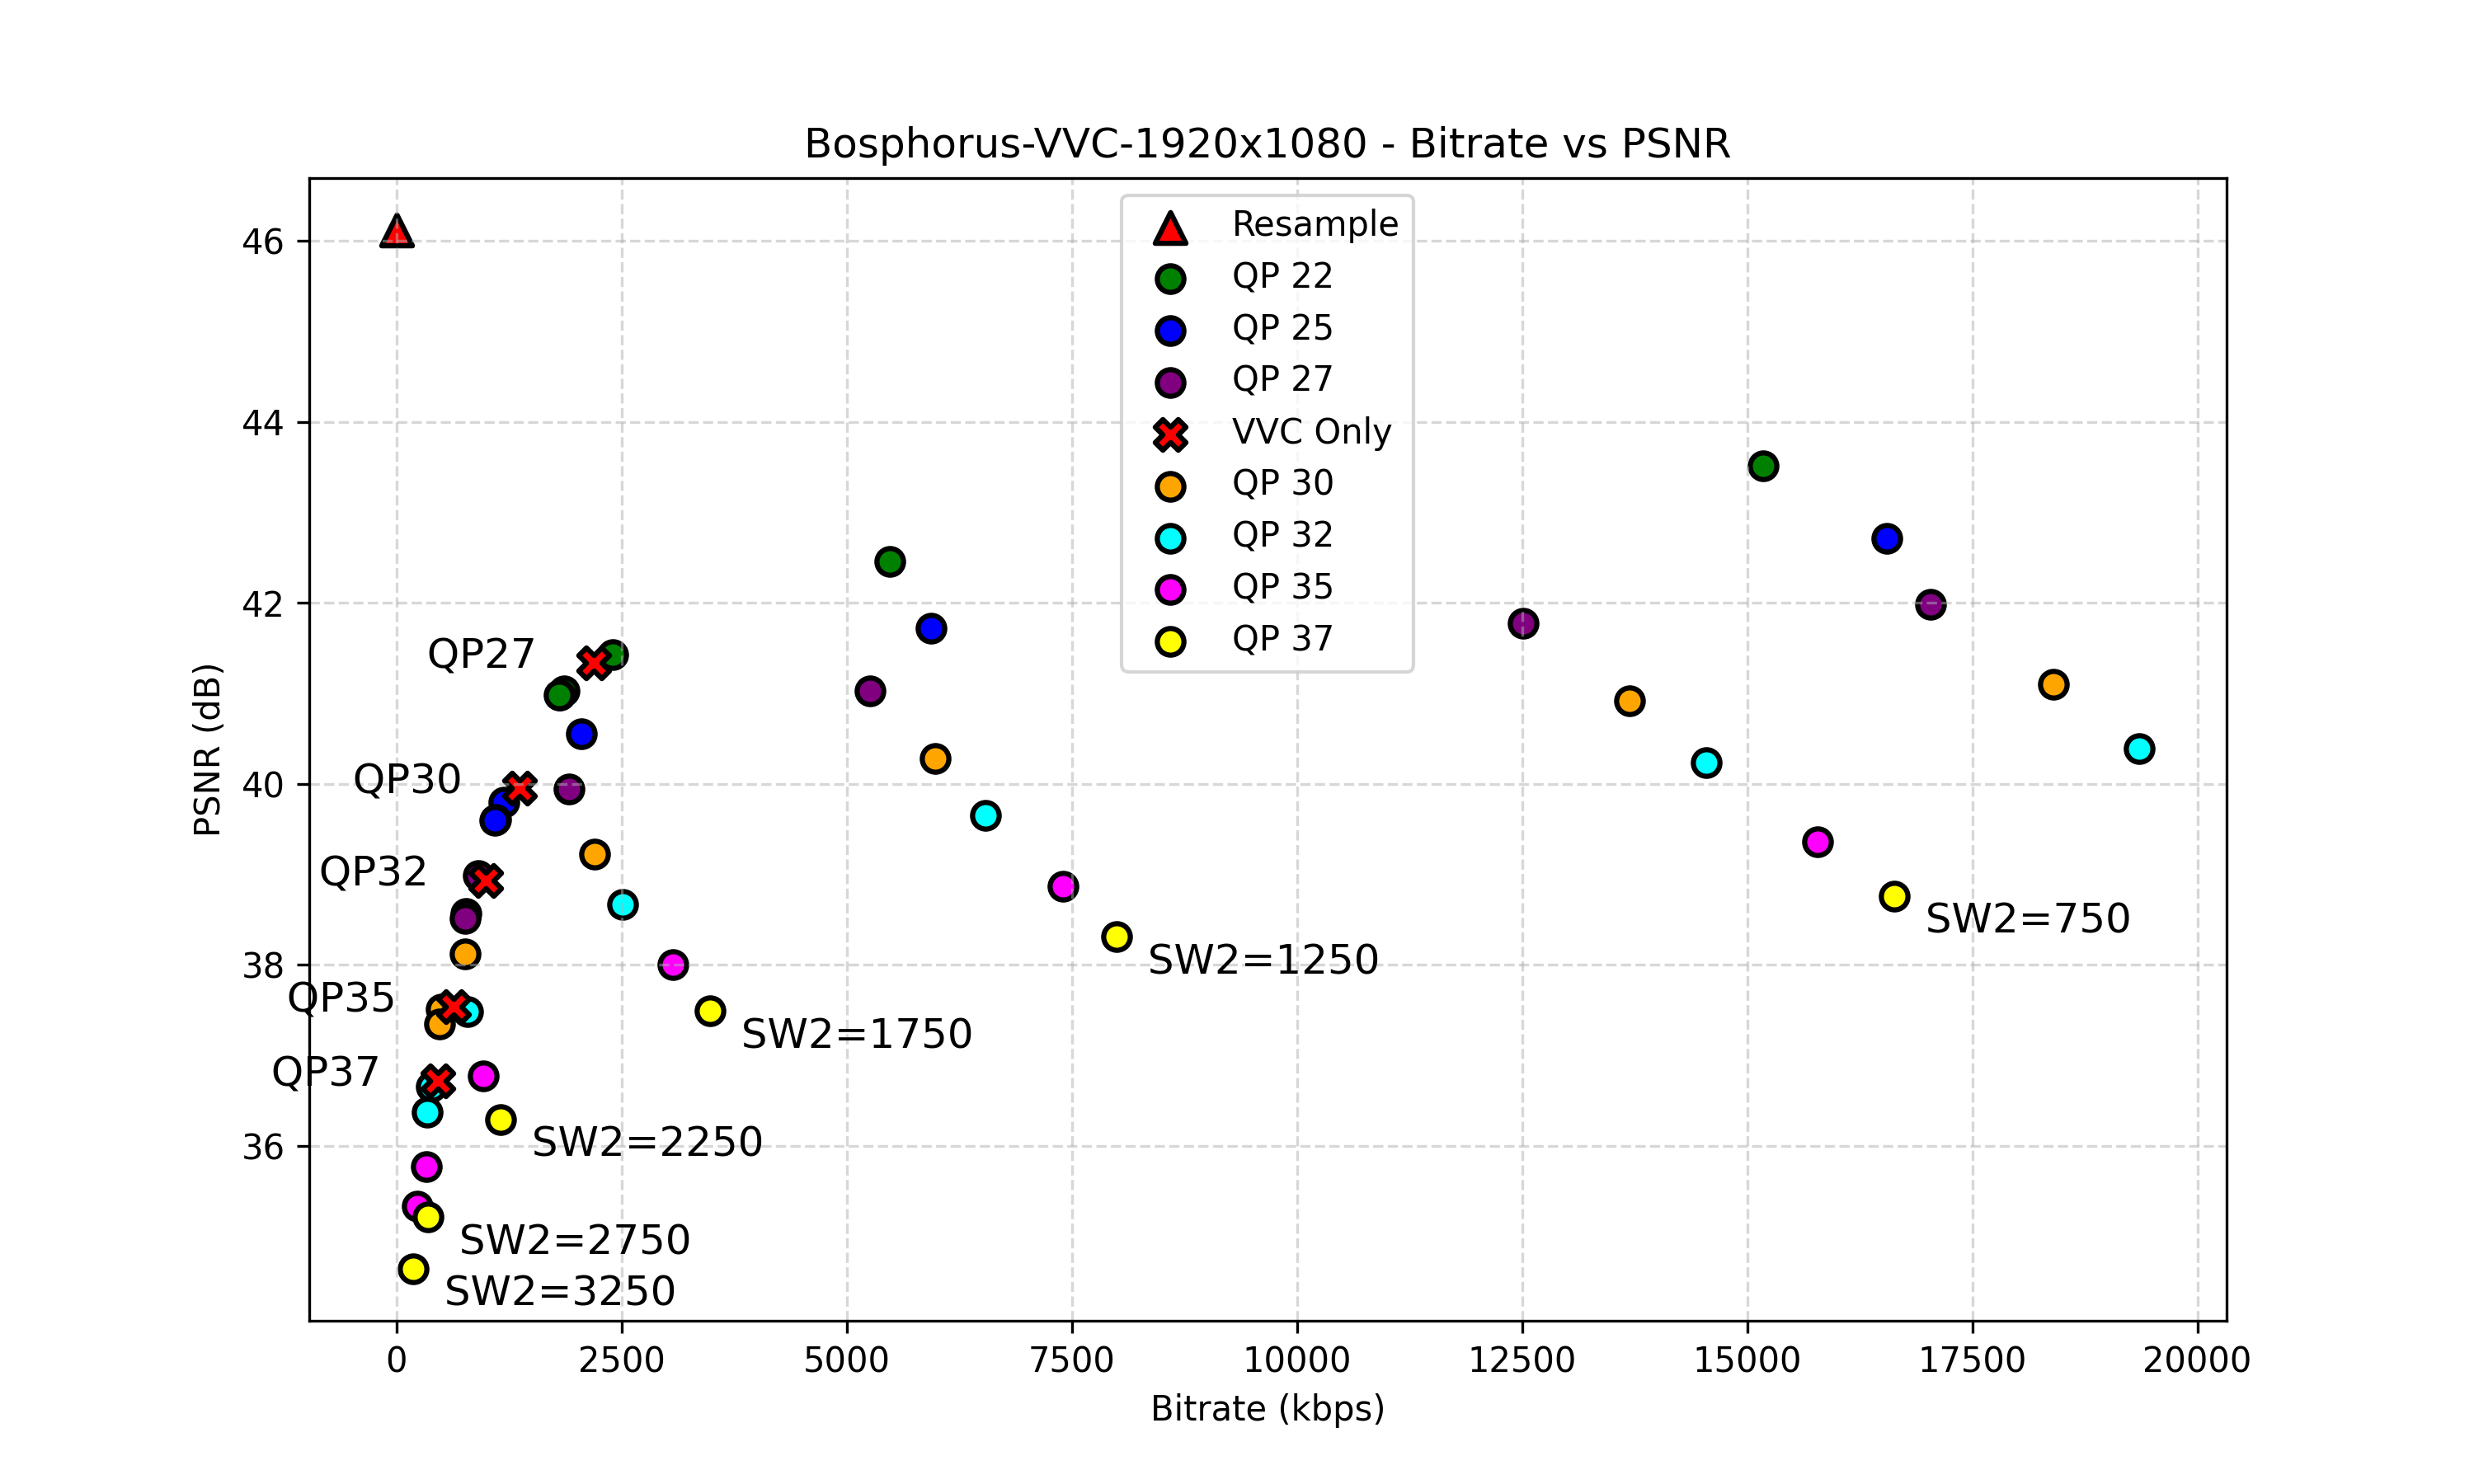
\includegraphics[width=1.0\textwidth]{img/Bosphorus-VVC.png}
    \caption{Resultados para "Bosphorus"\ em \acrshort{VVC}. \cite{uvg_dataset}}
    \label{fig:Bosphorus-VVC}
\end{figure}

Para o Bosphorus em \acrshort{VVC}, o \acrshort{LCEVC} também obteve bons resultados.
Vários pontos se encontram acima da curva dos vídeos somente em \acrshort{VVC}. Os 
valores para o QP que alcançaram estes pontos foram 30, 27, 25 e 22. Observa-se
que se a curva dos vídeos em \acrshort{VVC} mantenham a mesma tendência, haveriam
mais pontos favoráveis para o \acrshort{LCEVC}.

\begin{table}[h]
    \centering
    \begin{tabular}{|c|c|c|c|}
        \hline
        \textbf{QP} & \textbf{Tamanho (b)} & \textbf{PSNR (dB)} & \textbf{Taxa (kbps)} \\
        \hline
        37 & 580476 & 36.72 & 464.38 \\
        35 & 793851 & 37.54 & 635.08 \\
        32 & 1239951 & 38.93 & 991.96 \\
        30 & 1714361 & 39.95 & 1371.49 \\
        27 & 2738770 & 41.34 & 2191.02 \\
        \hline
    \end{tabular}
    \caption{Resultados para Bosphorus em VVC.}
    \label{tab:bosphorus-vvc}
\end{table}

\begin{table}[h]
    \centering
    \label{tab:bosphorus-vvc-lcevc}
    \begin{tabular}{|c|c|c|c|c|c|c|c|}
        \hline
        \textbf{SW2} & \textbf{QP} & \textbf{Tamanho (b)} & \textbf{Proporção} & \textbf{PSNR (dB)} & \textbf{Taxa (kbps)} & \textbf{Superou} \\
        \hline
        3250 & 30 & 594855 & 3.25\% & 37.35 & 475.88 & VVC QP37 \\
        2250 & 30 & 954971 & 39.74\% & 38.12 & 763.98 & VVC QP37 \\
        2750 & 30 & 621725 & 7.43\% & 37.51 & 497.38 & VVC QP35-32 \\
        3250 & 27 & 955429 & 1.73\% & 38.51 & 764.34 & VVC QP35-32 \\
        2750 & 27 & 965637 & 2.77\% & 38.57 & 772.51 & VVC QP35-32 \\
        2250 & 27 & 1132188 & 17.07\% & 38.99 & 905.75 & VVC QP35-32 \\
        2750 & 25 & 1373014 & 2.61\% & 39.61 & 1098.41 & VVC QP32-30 \\
        3250 & 25 & 1367475 & 2.22\% & 39.60 & 1093.98 & VVC QP32-30 \\
        2250 & 25 & 1487470 & 10.11\% & 39.80 & 1189.98 & VVC QP32-30 \\
        2750 & 22 & 2264797 & 1.48\% & 40.98 & 1811.84 & VVC QP30-27 \\
        3250 & 22 & 2261661 & 1.34\% & 40.98 & 1809.33 & VVC QP30-27 \\
        \hline
    \end{tabular}
    \caption{Resultados favoráveis do LCEVC para Bosphorus em VVC.}
\end{table}

\newpage
\subsection{SOCCER}

\begin{figure}[h]
    \centering
    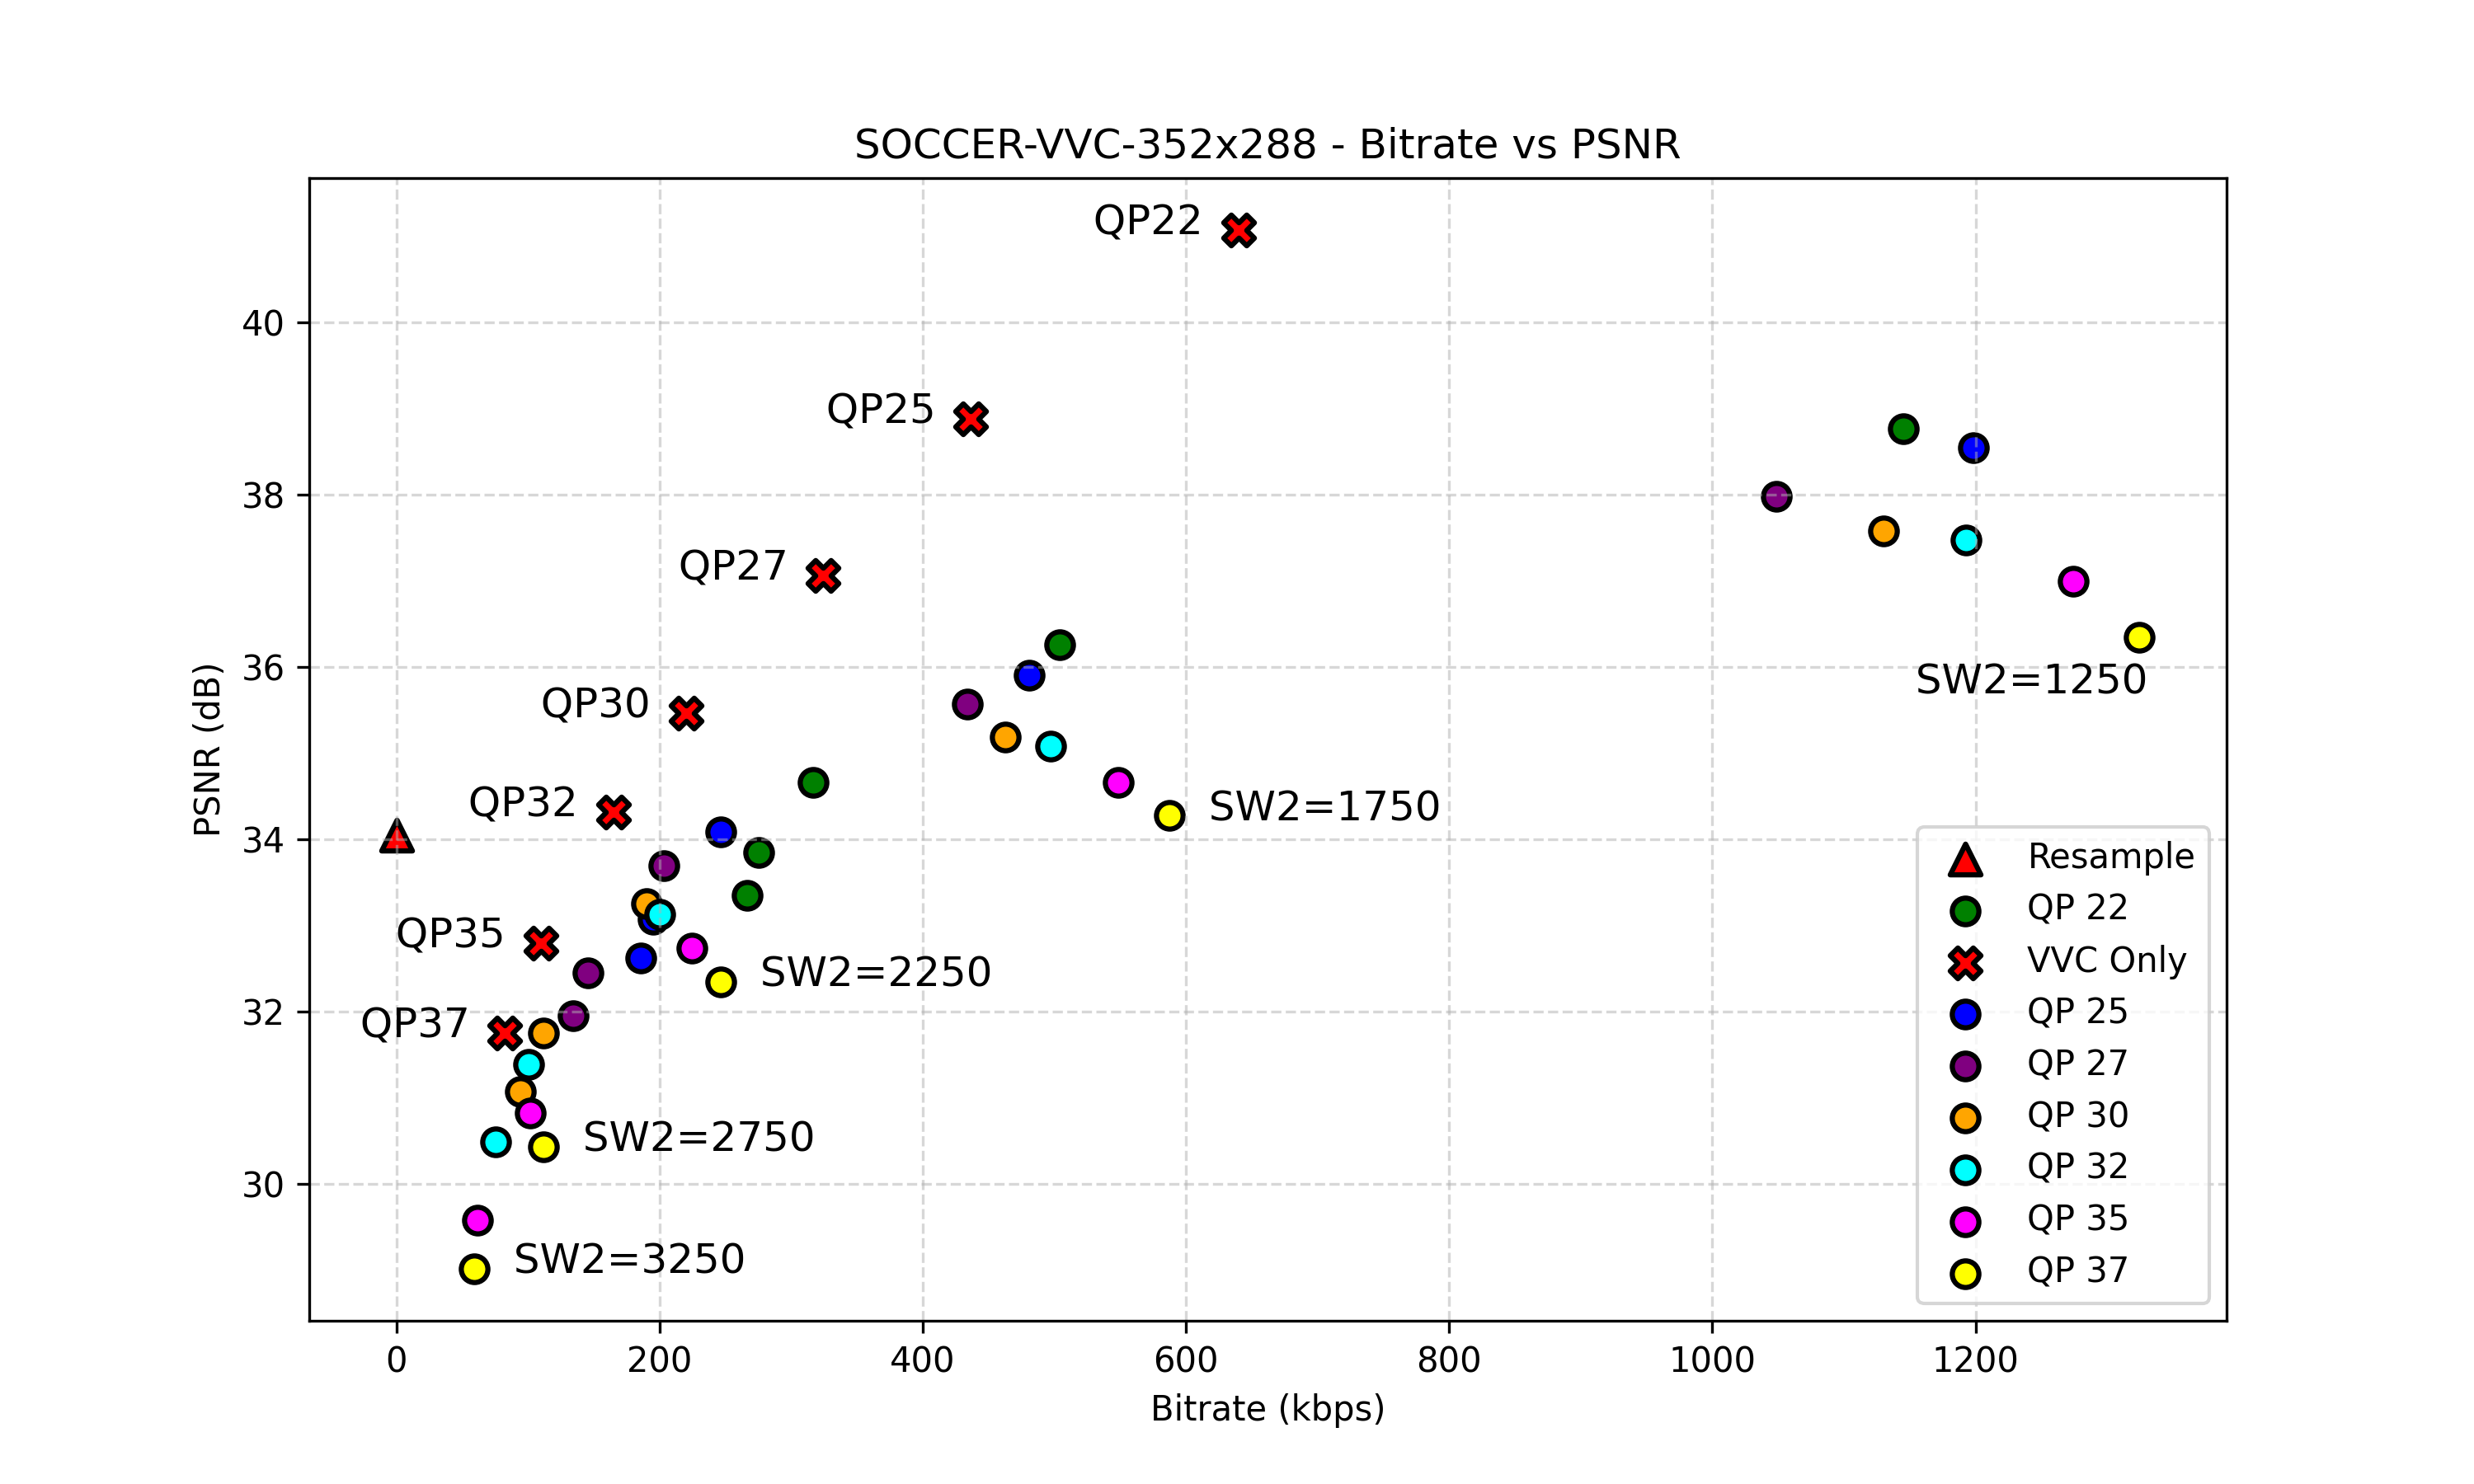
\includegraphics[width=01.0\textwidth]{img/SOCCER-VVC.png}
    \caption{Resultados para "SOCCER"\ em \acrshort{VVC}. \cite{xiph}}
    \label{fig:Soccer-VVC}
\end{figure}

Os resultados demonstram que neste caso houve uma vantagem para o uso de
somente o \acrshort{VVC}, com desempenho superior em todas as configurações testadas.
O \acrshort{LCEVC} demonstrou que nesta sequência, para os maiores valores de SW2 escolhidos, ele foi
capaz de chegar próximo a relação de tamanho e qualidade que o \acrshort{VVC} conseguiu,
porém não conseguiu superá-lo e foi se distanciando dos pontos obtidos pelo \acrshort{VVC}. 

\newpage
\subsection{Jockey}

\begin{figure}[h]
    \centering
    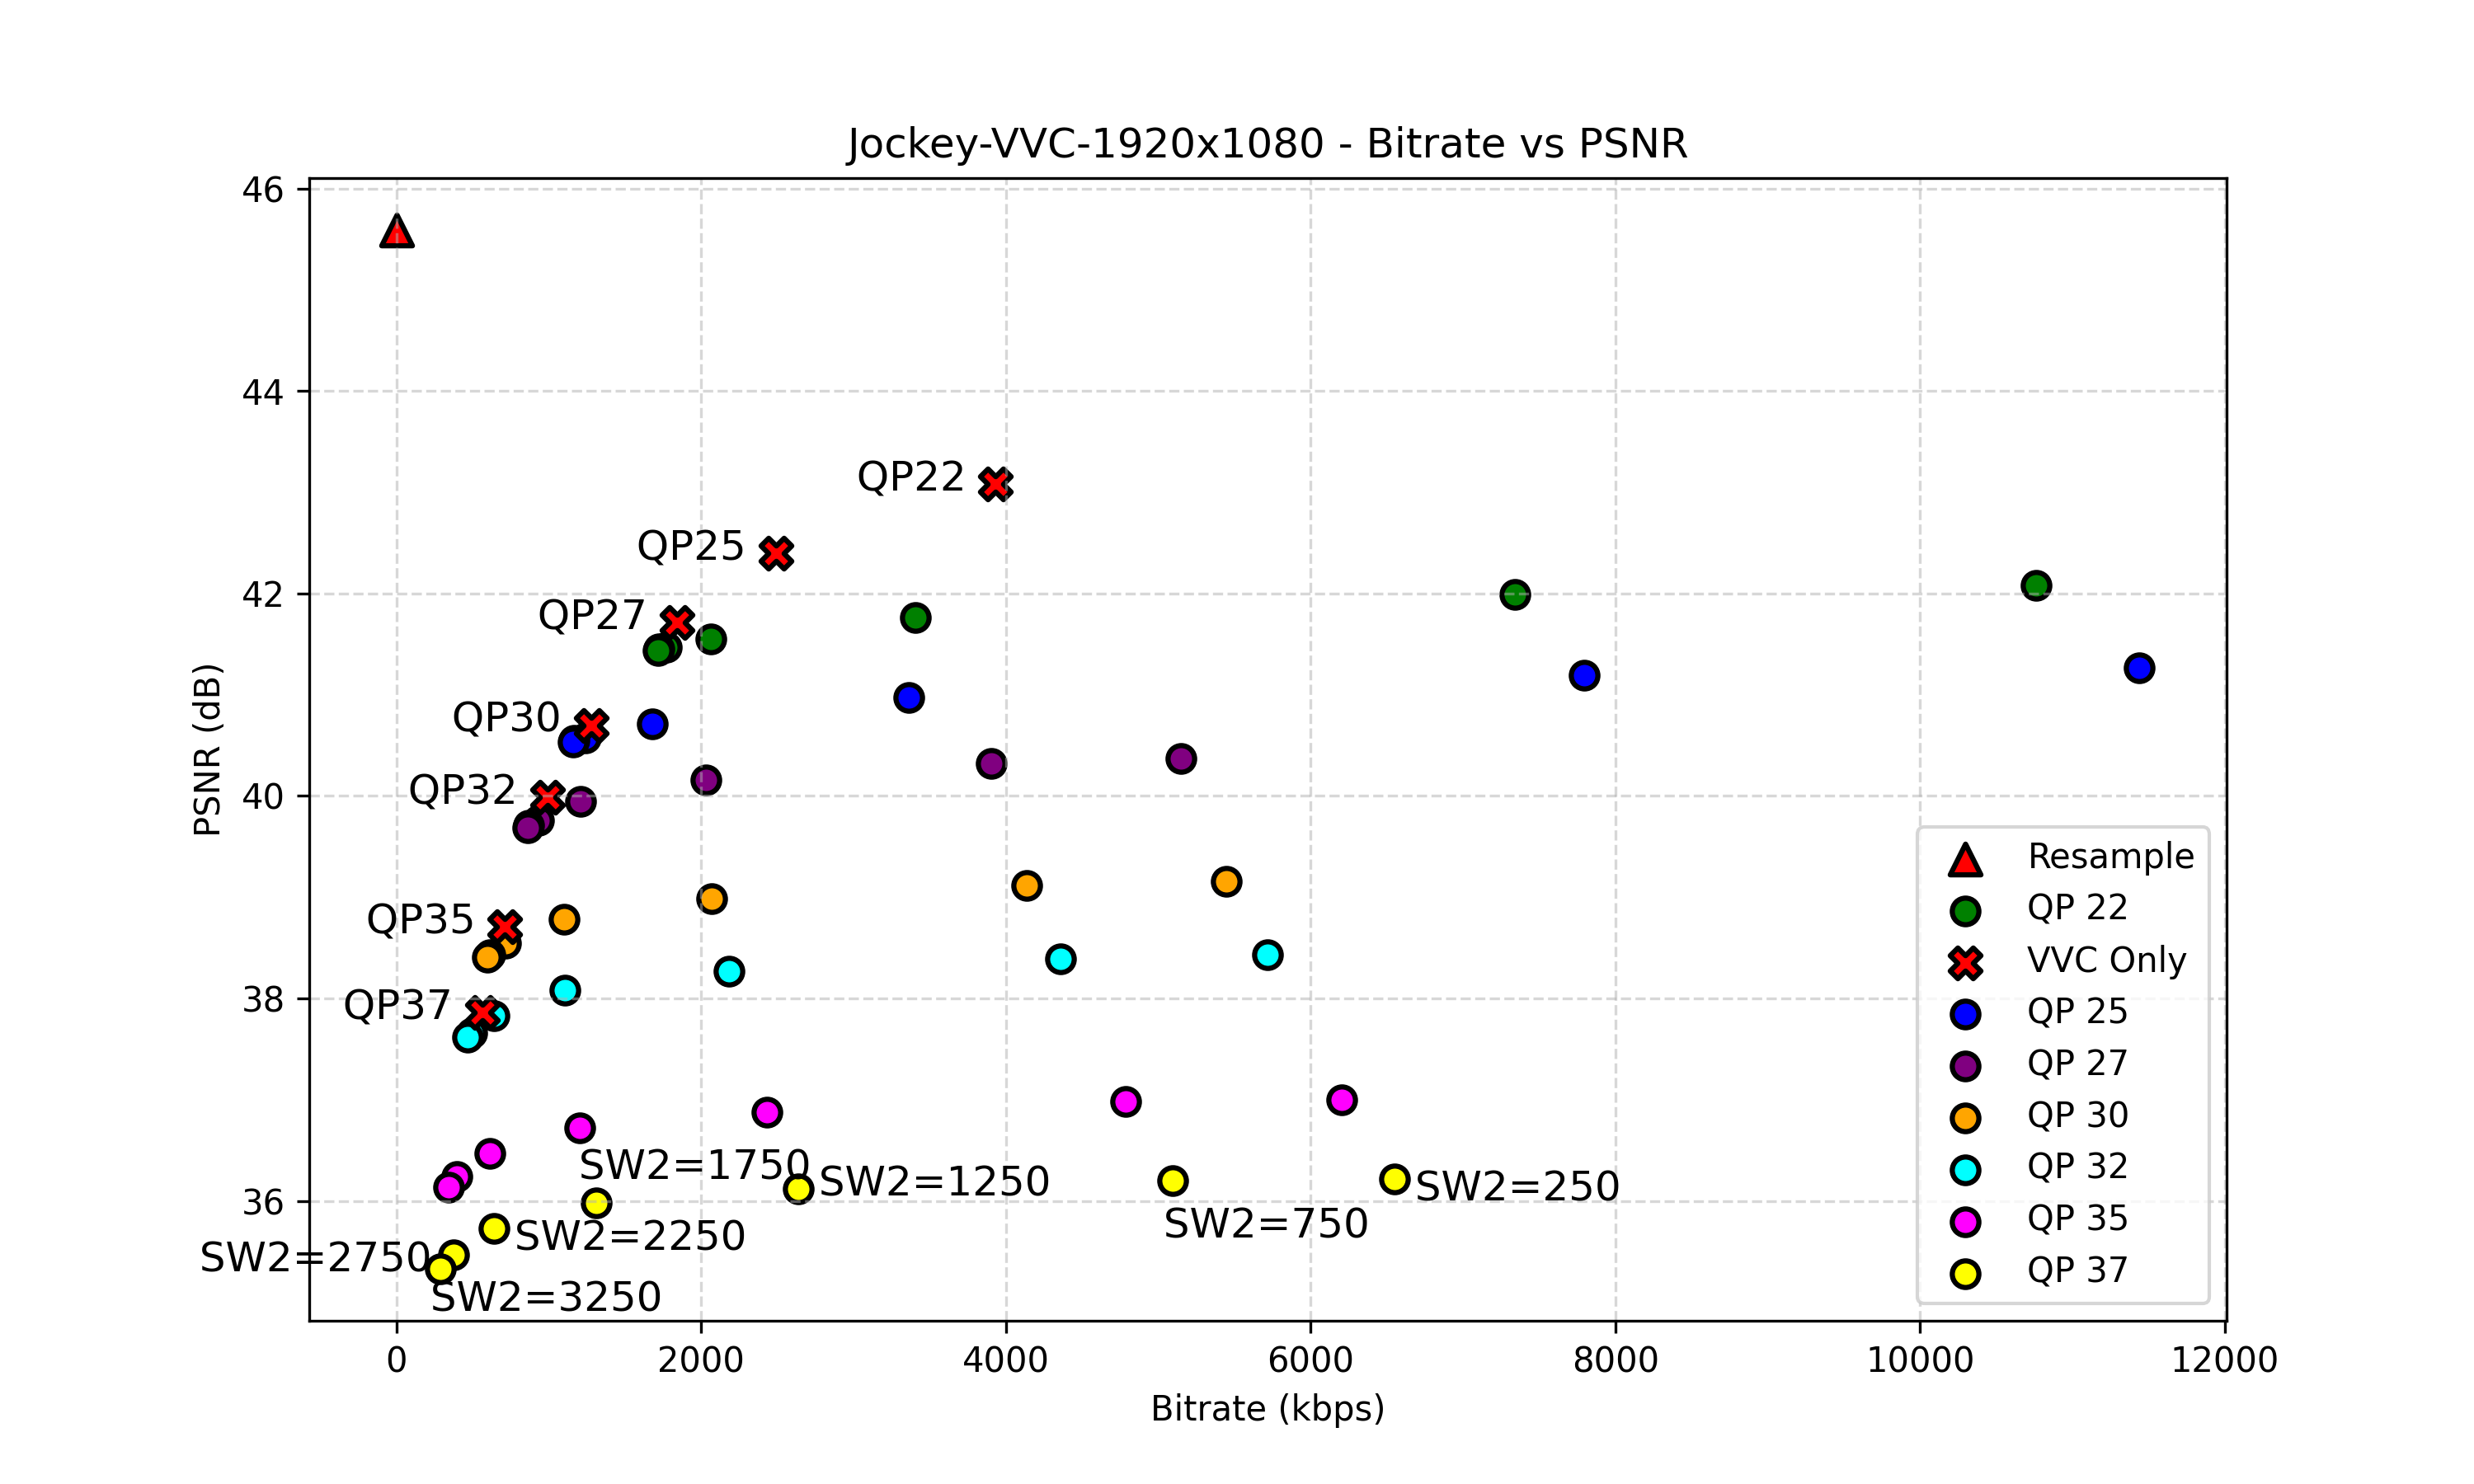
\includegraphics[width=1.0\textwidth]{img/Jockey-VVC.png}
    \caption{Resultados para "Jockey"\ em \acrshort{VVC}. \cite{uvg_dataset}}
    \label{fig:Jockey-VVC}
\end{figure}

Para esta sequência, o \acrshort{LCEVC} obteve bons resultados acima da curva de eficiência
obtida pelo \acrshort{VVC} puro. Valores para QPs iguais a 30, 27, 25 se saíram bem e estão
acima da curva. QP igual a 22 ficou bastante próximo, mostrando ser um resultado com potencial,
onde a qualidade e o tamanho destes arquivos estão próximos ao QP 27 do \acrshort{VVC}.

\begin{table}[h]
    \centering
    \begin{tabular}{|c|c|c|c|}
        \hline
        \textbf{QP} & \textbf{Tamanho (b)} & \textbf{PSNR (dB)} & \textbf{Taxa (kbps)} \\
        \hline
        37 & 704469 & 37.86 & 563.58 \\
        35 & 891197 & 38.71 & 712.96 \\
        32 & 1241194 & 39.99 & 992.96 \\
        30 & 1598336 & 40.70 & 1278.67 \\
        27 & 2300814 & 41.71 & 1840.65 \\
        25 & 3111449 & 42.40 & 2489.16 \\
        22 & 4916006 & 43.08 & 3932.80 \\
        \hline
    \end{tabular}
    \caption{Resultados para Jockey em VVC}
    \label{tab:jockey-vvc}
\end{table}

\begin{table}[h]
    \centering
    \label{tab:jockey-vvc-lcevc}
    \begin{tabular}{|c|c|c|c|c|c|c|c|}
        \hline
        \textbf{SW2} & \textbf{QP} & \textbf{Tamanho (b)} & \textbf{Proporção} & \textbf{PSNR (dB)} & \textbf{Taxa (kbps)} & \textbf{Superou} \\
        \hline
        3250 & 30 & 747523 & 2.48\% & 38.41 & 598.02 & VVC QP37 \\
        2750 & 30 & 765746 & 4.80\% & 38.43 & 612.60 & VVC QP37 \\
        3250 & 27 & 1075071 & 1.59\% & 39.69 & 860.06 & VVC QP35-32 \\
        2750 & 27 & 1083226 & 2.33\% & 39.71 & 866.58 & VVC QP35-32 \\
        2250 & 27 & 1162481 & 8.99\% & 39.76 & 929.98 & VVC QP35-32 \\
        3250 & 25 & 1449506 & 2.17\% & 40.53 & 1159.60 & VVC QP32-30 \\
        2750 & 25 & 1456646 & 2.65\% & 40.55 & 1165.32 & VVC QP32-30 \\
        \hline
    \end{tabular}
    \caption{Resultados favoráveis do LCEVC para Jockey em VVC.}
\end{table}

\newpage
\subsection{City}

\begin{figure}[h]
    \centering
    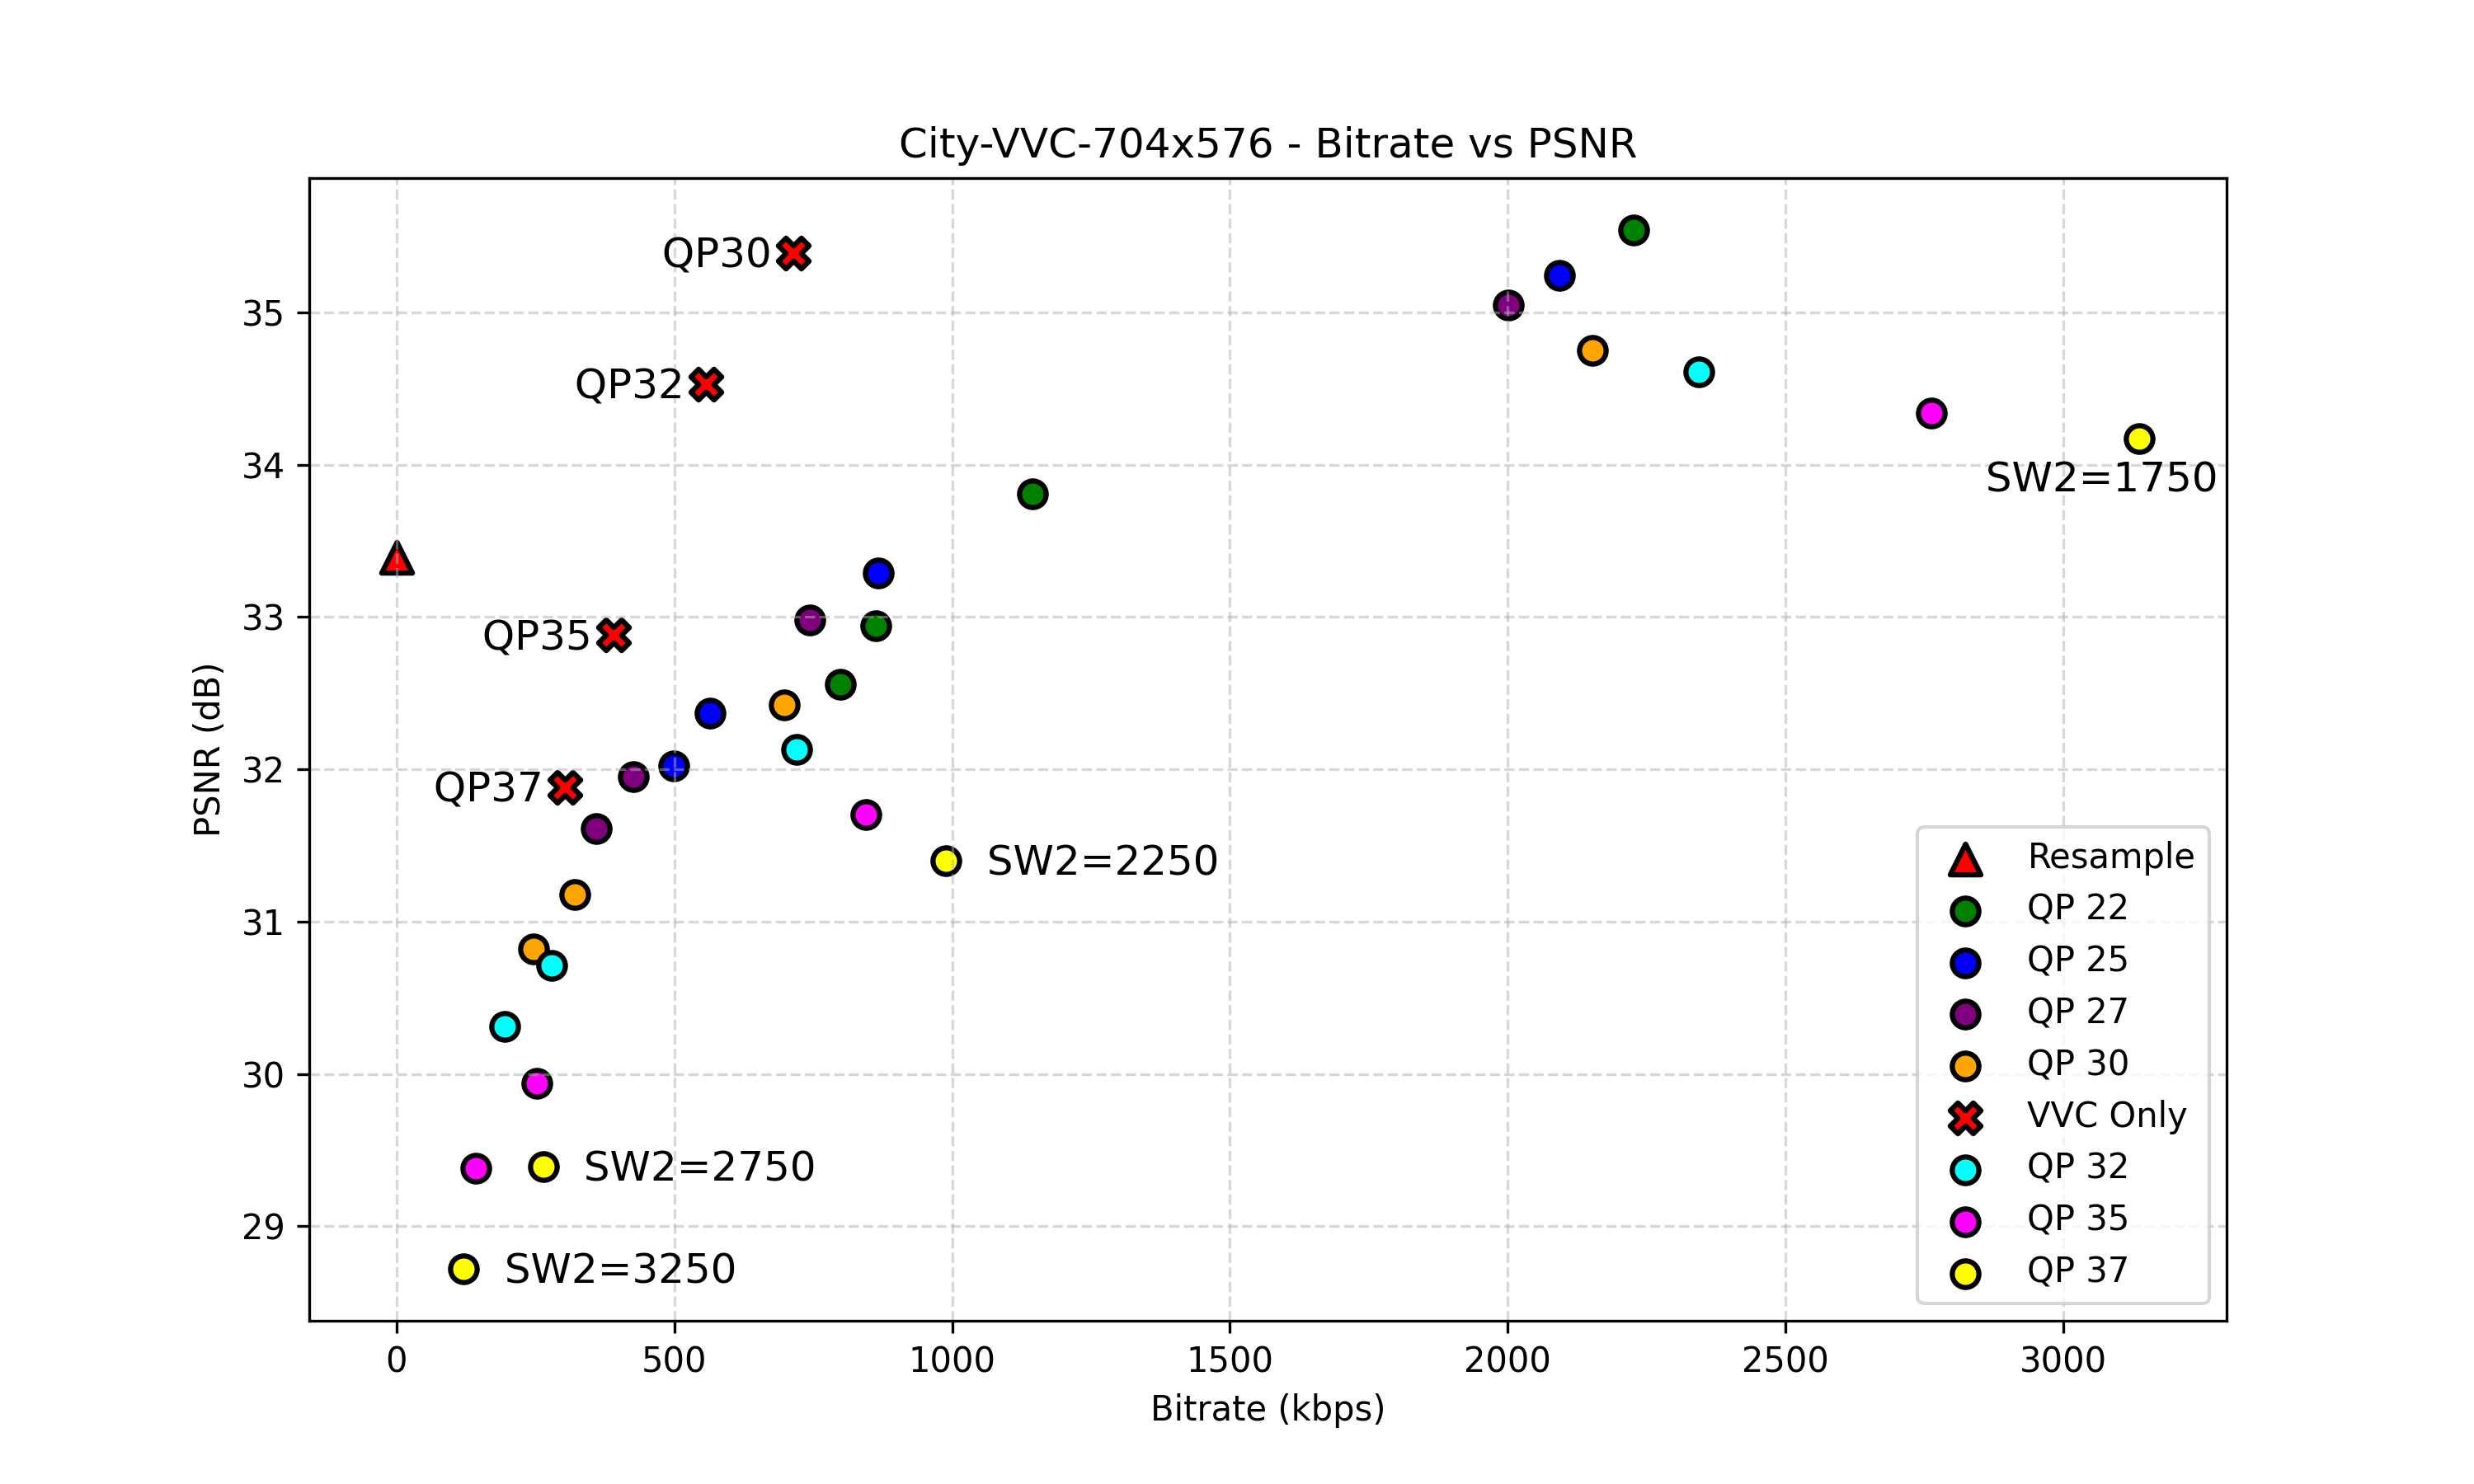
\includegraphics[width=1.0\textwidth]{img/City-VVC.png}
    \caption{Resultados para "City"\ em \acrshort{VVC}. \cite{xiph}}
    \label{fig:City-VVC}
\end{figure}

Em City, o \acrshort{LCEVC} não conseguiu superar os resultados obtidos com o \acrshort{VVC}.
Os resultados aparentam estar seguindo a mesma tendência que os resultados de referência no
início, mas começam a decair ao chegarem perto do \acrshort{VVC} QP37. Com ess
e decaimento, 
se distanciam cada vez mais e não conseguem um resultado satisfatório.

\newpage

\subsection{vc-philips-01}

\begin{figure}[h]
    \centering
    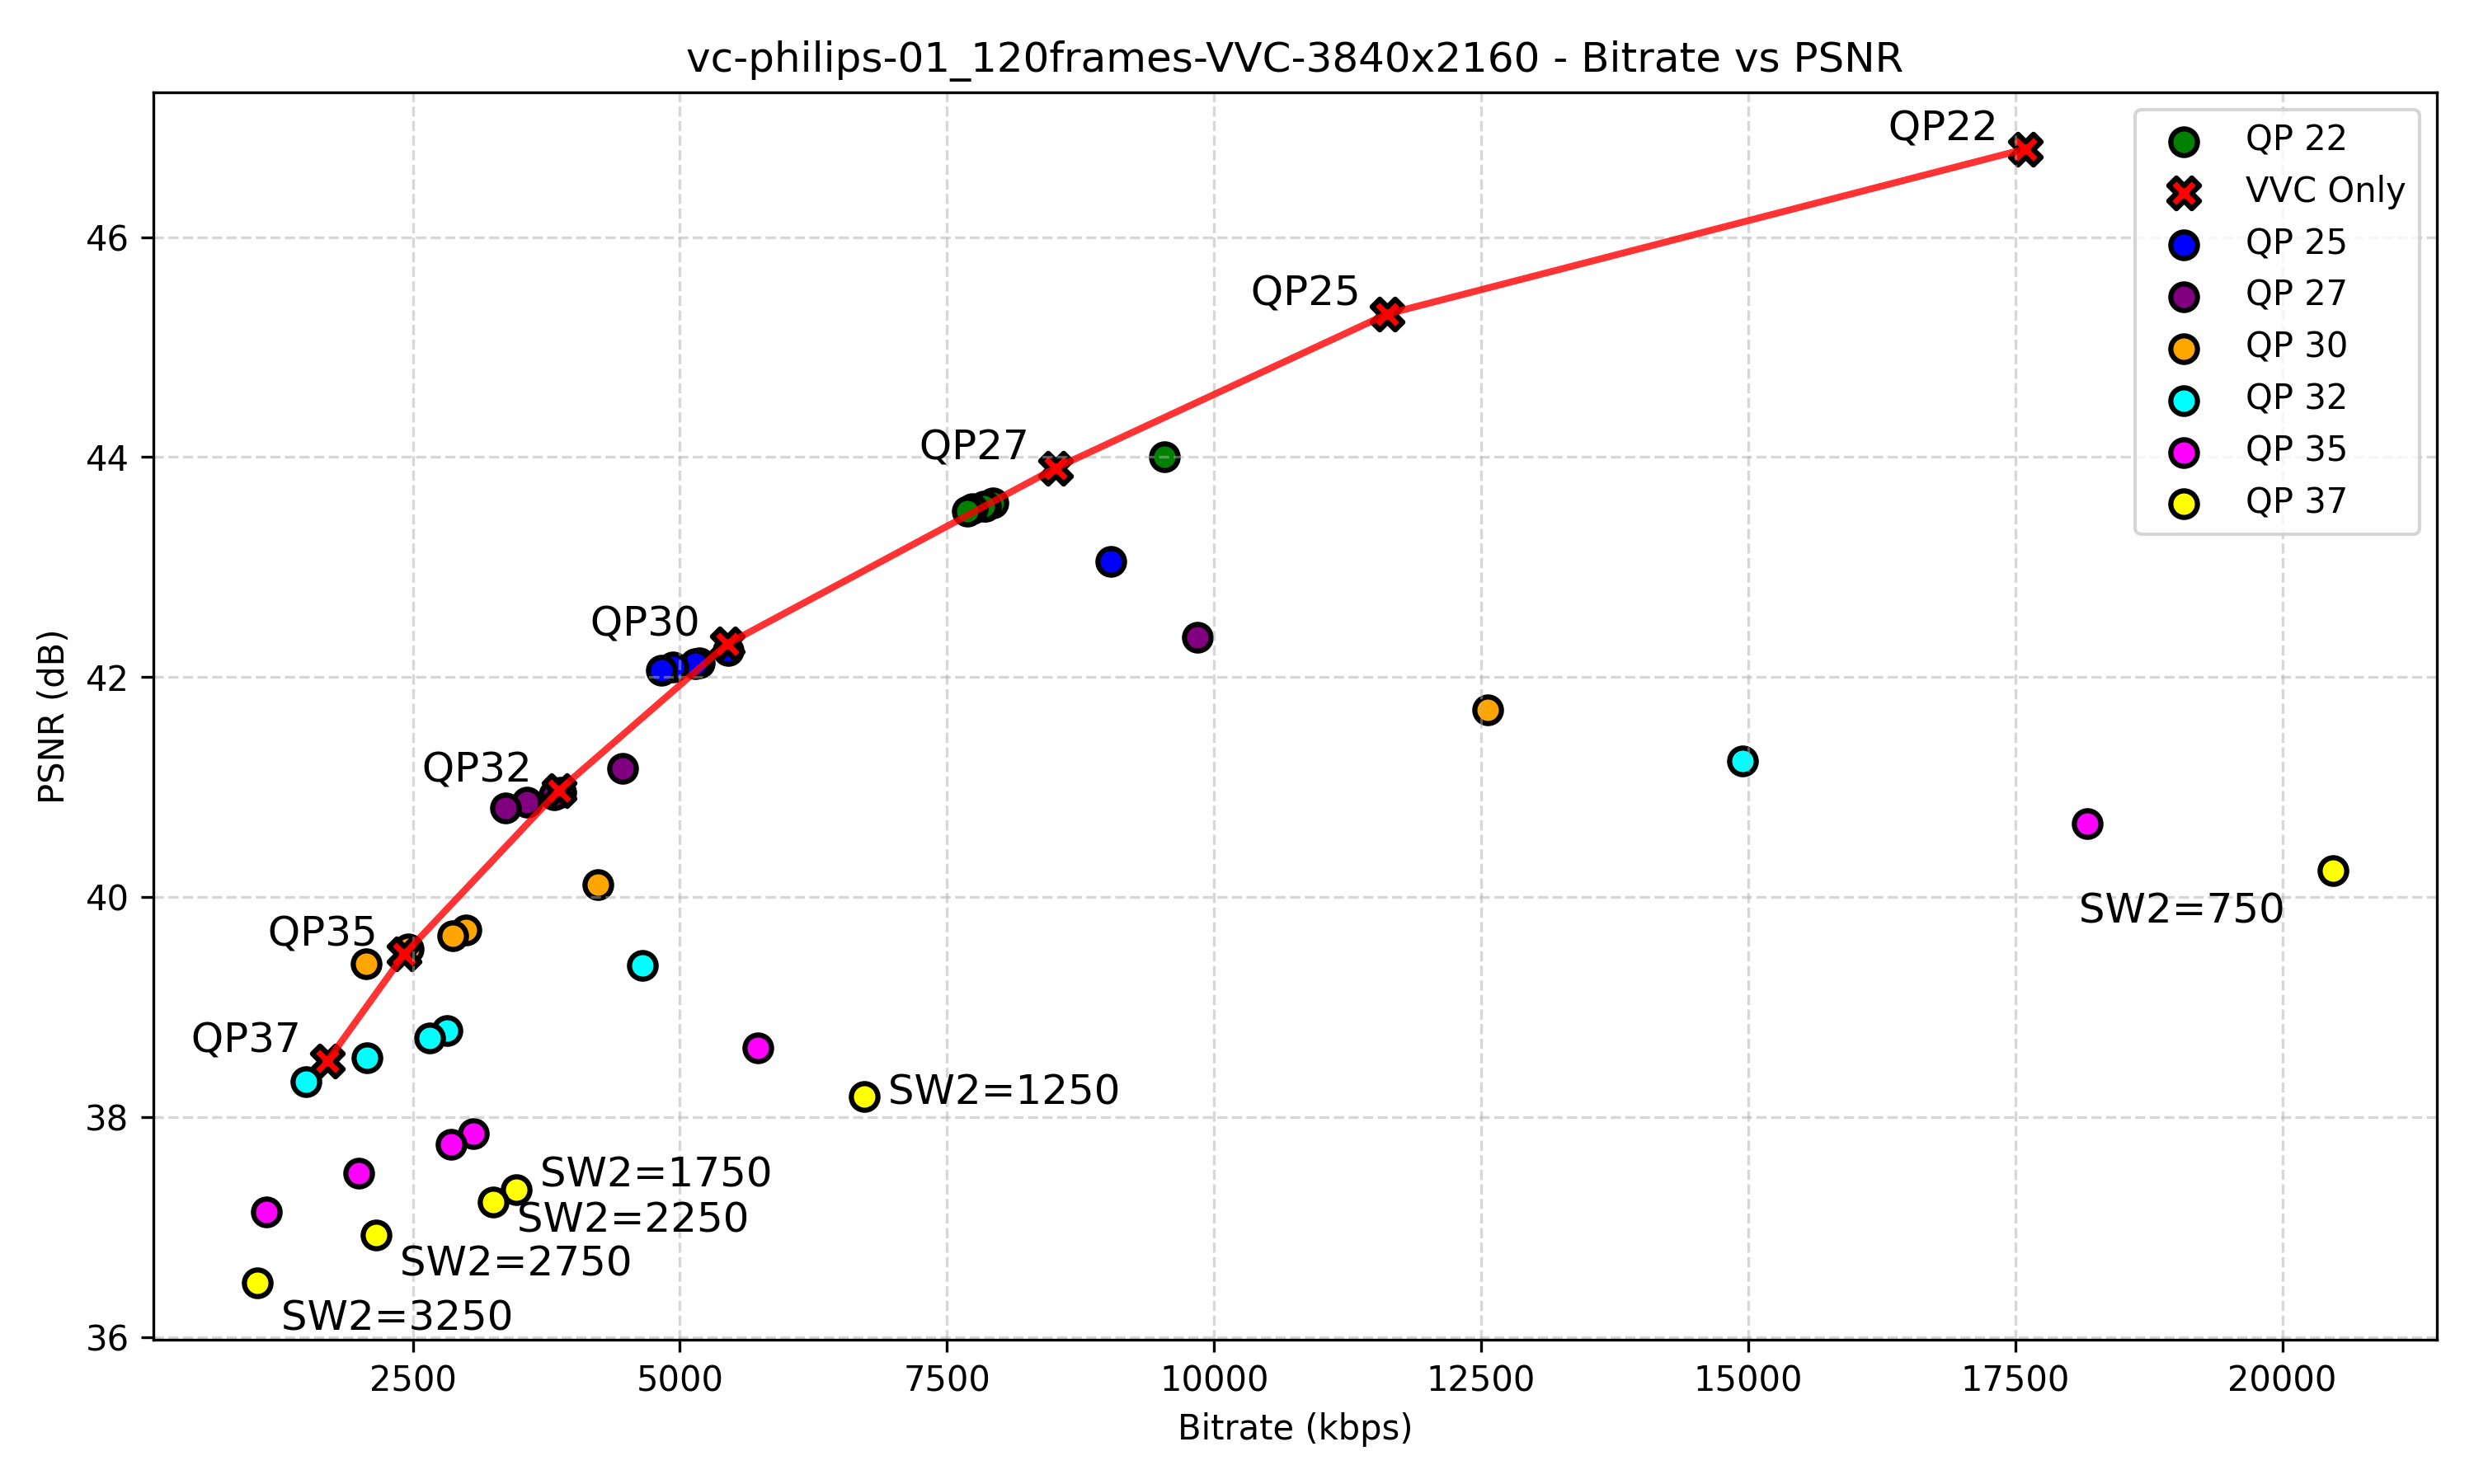
\includegraphics[width=1.0\textwidth]{img/vc-philips-01_120frames-VVC.png}
    \caption{Resultados para "vc-philips-01"\ em \acrshort{VVC}.}
    \label{fig:vc-philips-01-VVC}
\end{figure}

Esta sequência obteve uma quantidade considerável de resultados positivos para o \acrshort{LCEVC}, para valores de
QP iguais 30, 27, 25 e 22. Para o QP 22, observa-se que o \acrshort{LCEVC} obteve
vários valores em cima da curva de eficiência das sequências de referência, onde
pela tendência observada, é possível que os resultados para um QP menor que 22 iria
resultar em resultados abaixo da curva de eficiência.

\begin{table}[h]
    \centering
    \begin{tabular}{|c|c|c|c|}
        \hline
        \textbf{QP} & \textbf{Tamanho (b)} & \textbf{PSNR (dB)} & \textbf{Taxa (kbps)} \\
        \hline
        37 & 425336 & 38.51 & 1701.34 \\
        35 & 604903 & 39.48 & 2419.61 \\
        32 & 966774 & 40.97 & 3867.10 \\
        30 & 1360536 & 42.30 & 5442.14 \\
        27 & 2129169 & 43.90 & 8516.68 \\
        25 & 2905023 & 45.30 & 11620.09 \\
        22 & 4397908 & 46.80 & 17591.63 \\
        \hline
    \end{tabular}
    \caption{Resultados para vc-philips-01 em VVC.}
    \label{tab:vc-philips-01-vvc}
\end{table}

\newpage
\begin{table}[h]
    \centering
    \label{tab:vc-philips-01-vvc-lcevc}
    \begin{tabular}{|c|c|c|c|c|c|c|c|}
        \hline
        \textbf{SW2} & \textbf{QP} & \textbf{Tamanho (b)} & \textbf{Proporção} & \textbf{PSNR (dB)} & \textbf{Taxa (kbps)} & \textbf{Superou} \\
        \hline
        3250 & 30 & 516071 & 5.39\% & 39.39 & 2064.28 & VVC QP37-35 \\
        2750 & 30 & 613763 & 20.45\% & 39.53 & 2455.05 & VVC QP35 \\
        3250 & 27 & 842020 & 1.12\% & 40.81 & 3368.08 & VVC QP35-32 \\
        2750 & 27 & 891745 & 6.63\% & 40.86 & 3566.98 & VVC QP35-32 \\
        2250 & 27 & 955257 & 12.84\% & 40.93 & 3821.03 & VVC QP35-32 \\
        1750 & 27 & 971277 & 14.28\% & 40.95 & 3885.11 & VVC QP35-32 \\
        3250 & 25 & 1205943 & 0.50\% & 42.06 & 4823.77 & VVC QP32-30 \\
        2750 & 25 & 1234327 & 2.78\% & 42.09 & 4937.31 & VVC QP32-30 \\
        2250 & 25 & 1286043 & 6.69\% & 42.12 & 5144.17 & VVC QP32-30 \\
        1750 & 25 & 1295331 & 7.36\% & 42.13 & 5181.32 & VVC QP32-30 \\
        3250 & 22 & 1922342 & 0.26\% & 43.51 & 7689.37 & VVC QP30-27 \\
        2750 & 22 & 1933946 & 0.86\% & 43.53 & 7735.78 & VVC QP30-27 \\
        2250 & 22 & 1961129 & 2.24\% & 43.55 & 7844.52 & VVC QP30-27 \\
        1250 & 22 & 1982576 & 3.29\% & 43.58 & 7930.30 & VVC QP30-27 \\
        1750 & 22 & 1965174 & 2.44\% & 43.55 & 7860.70 & VVC QP30-27 \\
        \hline
    \end{tabular}
    \caption{Resultados favoráveis do LCEVC para vc-philips-01 em VVC.}
\end{table}

\newpage
\subsection{vc-lcevc-01}

\begin{figure}[h]
    \centering
    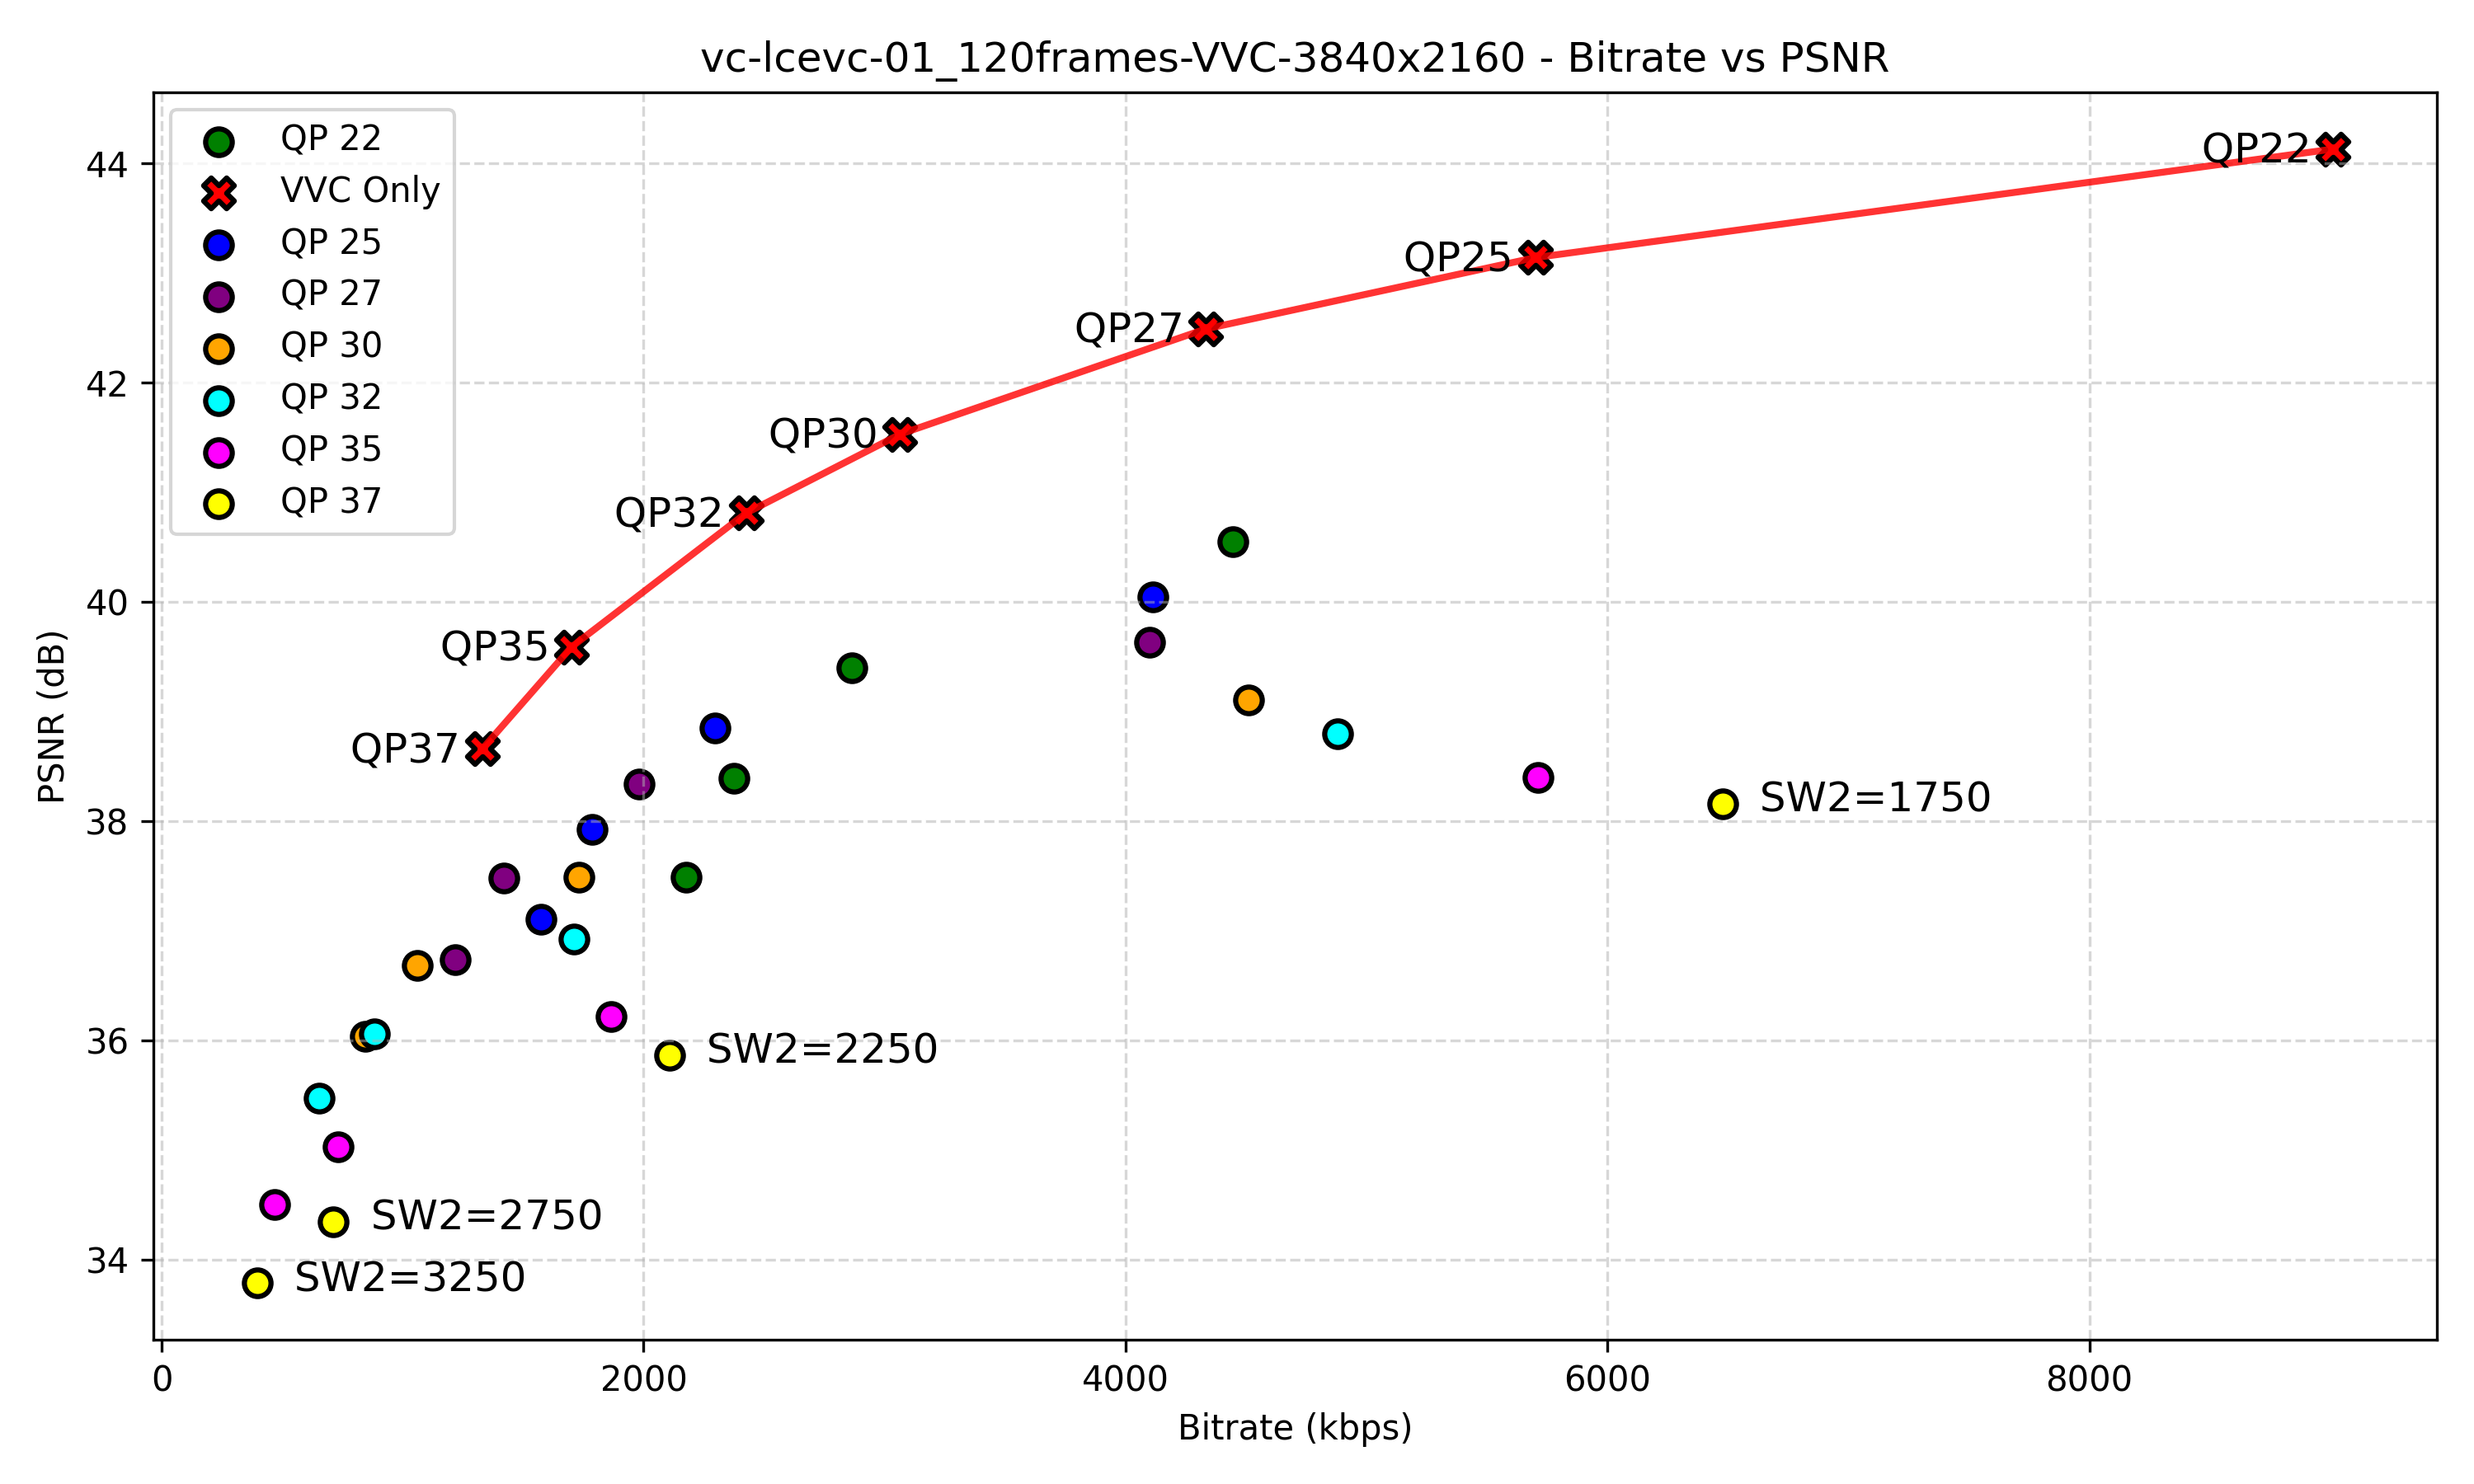
\includegraphics[width=1.0\textwidth]{img/vc-lcevc-01_120frames-VVC.png}
    \caption{Resultados para "vc-lcevc-01" em \acrshort{VVC}.}
    \label{fig:vc-lcevc-01-VVC}
\end{figure}

Para esta sequência, o \acrshort{LCEVC} não obteve resultados acima da curva de eficiência.
Os resultados para o \acrshort{LCEVC} ficaram relativamente distantes da curva de referência do 
\acrshort{VVC}. Ela aparenta um mesmo formato de curva, sugerindo que está mantendo a qualidade
da mesma maneira que o \acrshort{VVC} puro.

\newpage
\subsection{vc-globo-05}

\begin{figure}[h]
    \centering
    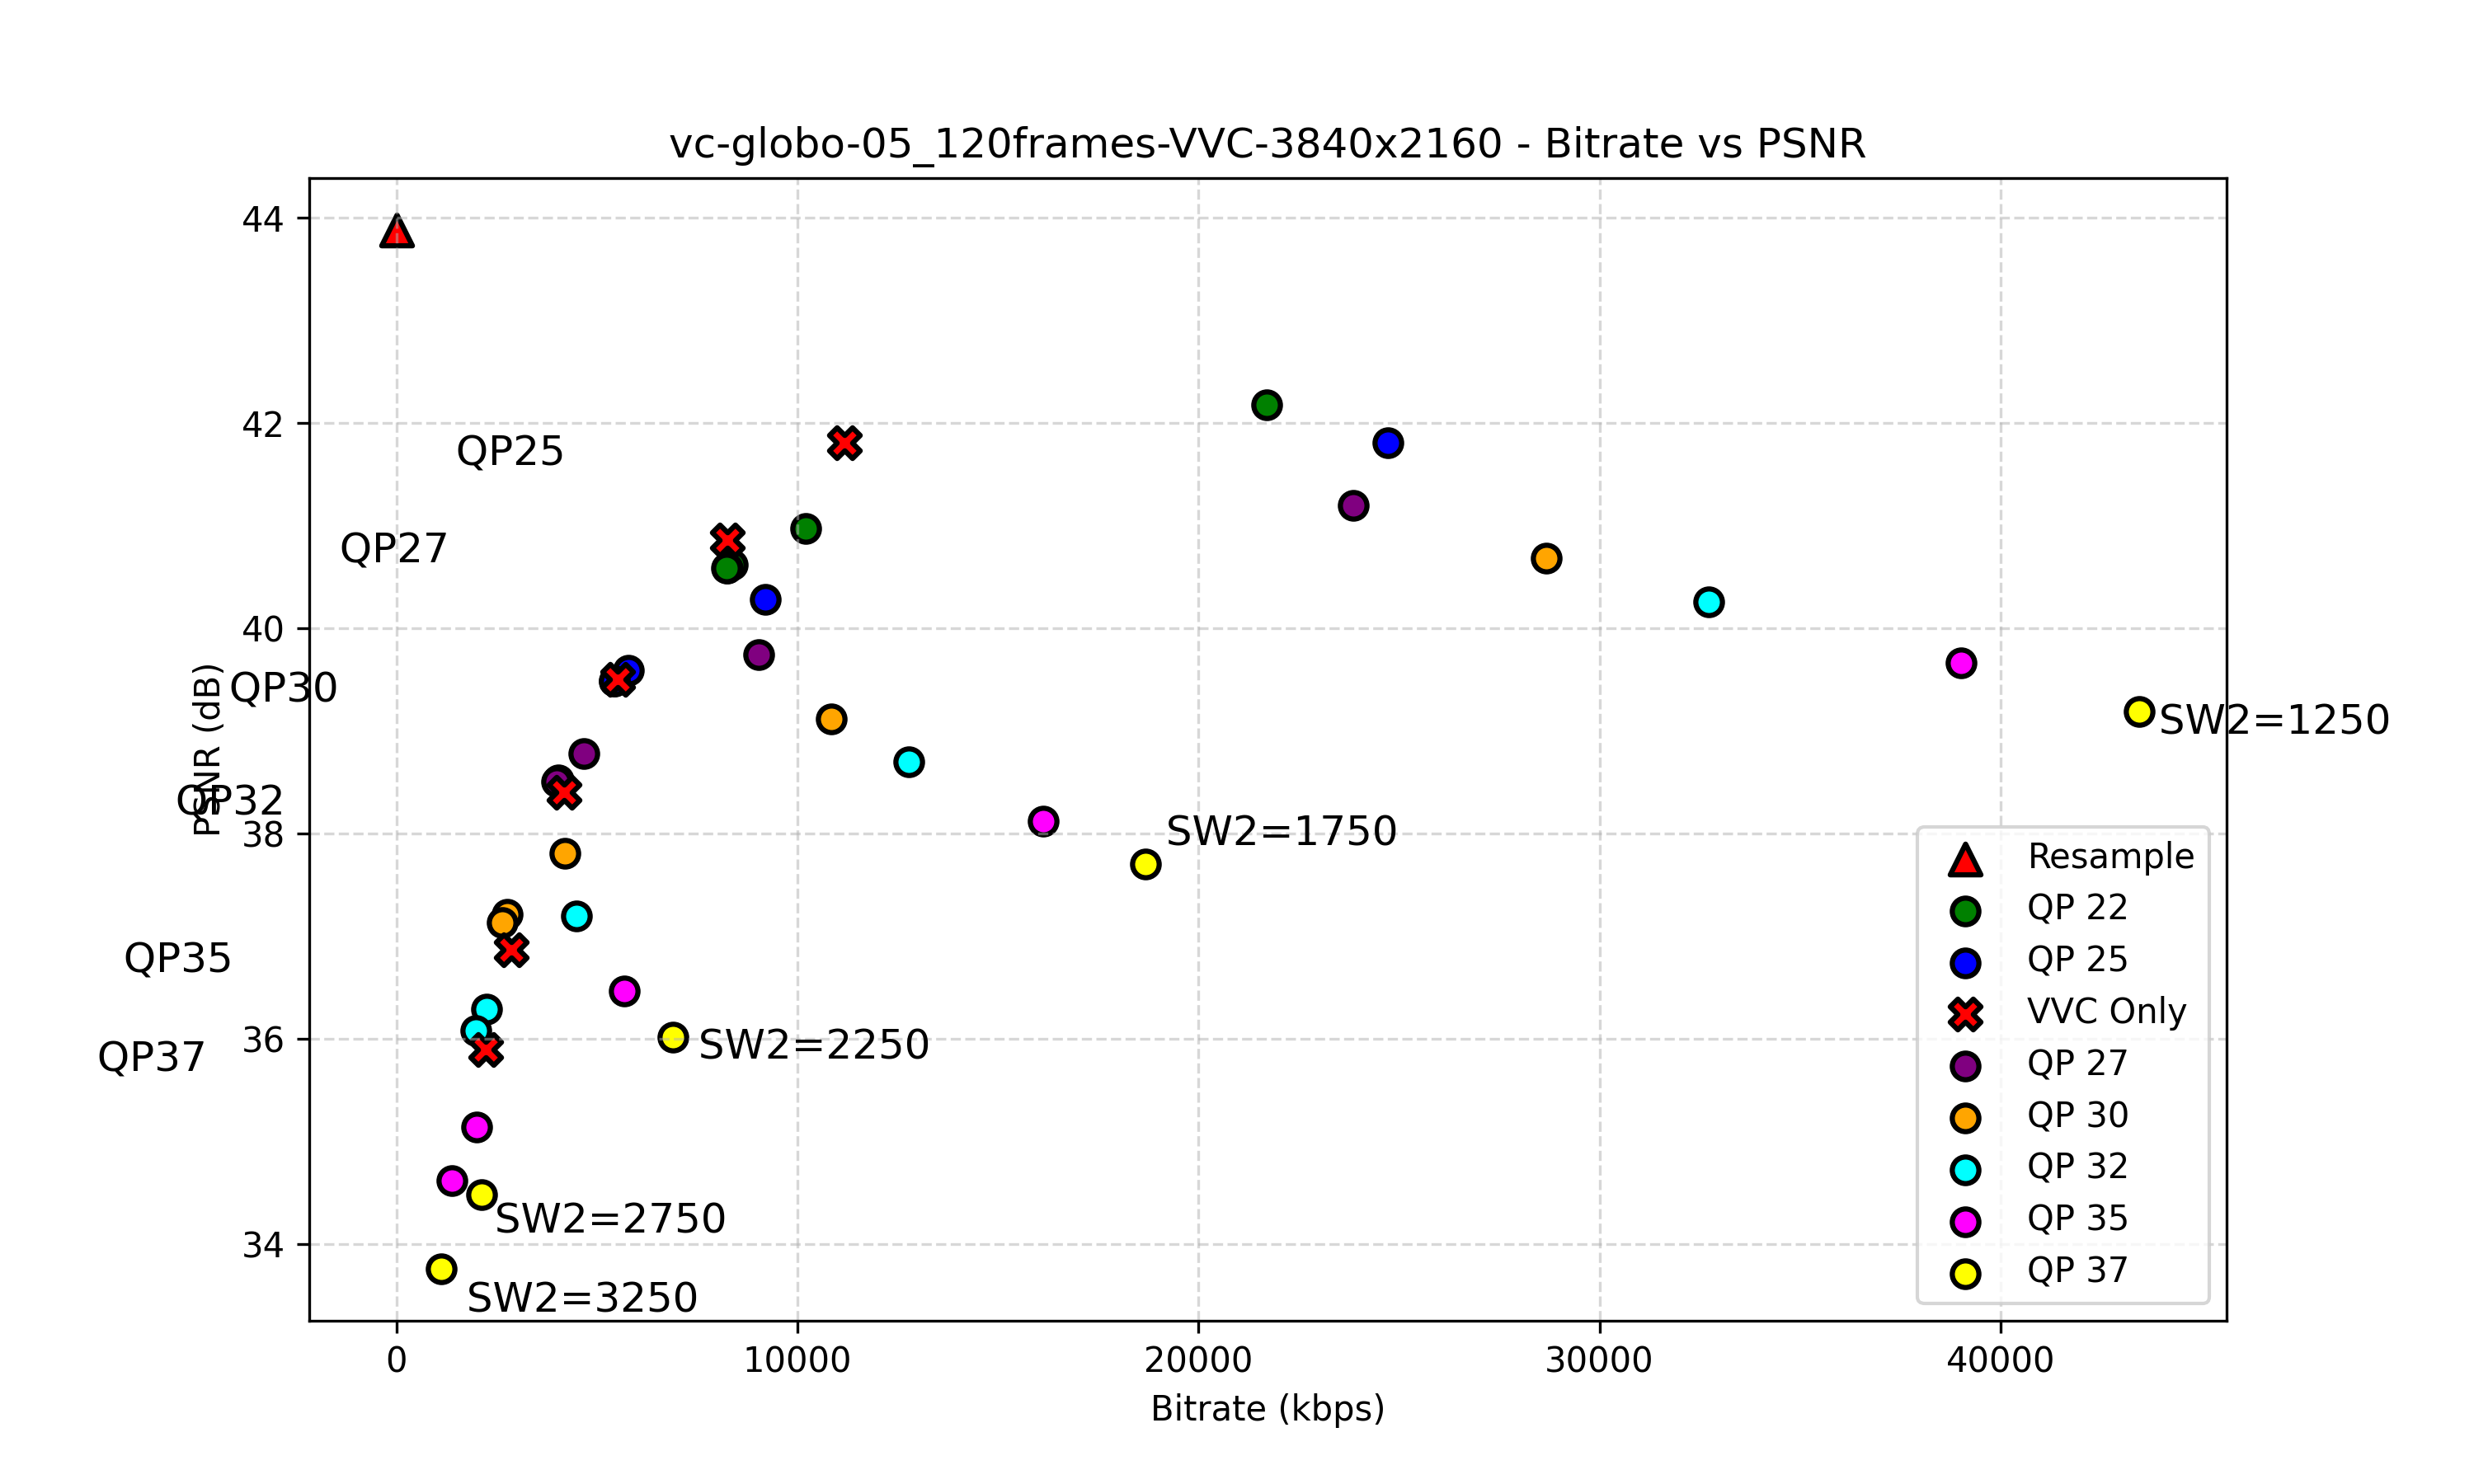
\includegraphics[width=1.0\textwidth]{img/vc-globo-05_120frames-VVC.png}
    \caption{Resultados para "vc-globo-05" em \acrshort{VVC} \cite{globo_video_uhd}.}
    \label{fig:vc-globo-05-VVC}
\end{figure}

Em \textit{vc-globo-05}, o \acrshort{LCEVC} obteve resultados positivos melhores que
os resultados obtidos pelo \acrshort{VVC}. Os valores de QP que conseguiram resultados
acima da curva foram 32, 30, 27 e 25. Para QP igual a 22, os resultados ficaram com o
valor de \acrshort{PSNR} levemente inferior ao QP 27 do \acrshort{VVC}, com a mesma
taxa de bits.

\begin{table}[h]
    \centering
    \begin{tabular}{|c|c|c|c|}
        \hline
        \textbf{QP} & \textbf{Tamanho (b)} & \textbf{PSNR (dB)} & \textbf{Taxa (kbps)} \\
        \hline
        37 & 554404 & 35.90 & 2217.62 \\
        35 & 715402 & 36.87 & 2861.61 \\
        32 & 1042958 & 38.40 & 4171.83 \\
        30 & 1377368 & 39.50 & 5509.47 \\
        27 & 2063711 & 40.86 & 8254.84 \\
        25 & 2790684 & 41.81 & 11162.74 \\
        \hline
    \end{tabular}
    \caption{Resultados para vc-globo-05 em VVC.}
    \label{tab:vc-globo-05-vvc}
\end{table}

\begin{table}[h]
    \centering
    \label{tab:vc-globo-05-vvc-lcevc}
    \begin{tabular}{|c|c|c|c|c|c|c|c|}
        \hline
        \textbf{SW2} & \textbf{QP} & \textbf{Tamanho (b)} & \textbf{Proporção} & \textbf{PSNR (dB)} & \textbf{Taxa (kbps)} & \textbf{Superou} \\
        \hline
        3250 & 32 & 495040 & 1.35\% & 36.08 & 1980.16 & VVC QP37 \\
        2750 & 32 & 561763 & 13.06\% & 36.29 & 2247.05 & VVC QP37 \\
        3250 & 30 & 660706 & 0.58\% & 37.13 & 2642.82 & VVC QP35 \\
        2750 & 30 & 689863 & 4.78\% & 37.21 & 2759.45 & VVC QP35 \\
        3250 & 27 & 1000292 & 0.31\% & 38.51 & 4001.17 & VVC QP32 \\
        2750 & 27 & 1007875 & 1.06\% & 38.52 & 4031.50 & VVC QP32 \\
        3250 & 25 & 1356490 & 0.44\% & 39.49 & 5425.96 & VVC QP30 \\
        2750 & 25 & 1359403 & 0.66\% & 39.49 & 5437.61 & VVC QP30 \\
        \hline
    \end{tabular}
    \caption{Resultados favoráveis do LCEVC para vc-globo-05 em VVC.}
\end{table}

\newpage
\section{Visão geral dos resultados}

Com os estes resultados obtidos, as tabelas abaixo demonstram a quantidade de pontos
favoráveis para o \acrshort{LCEVC} para cada sequência.

\begin{table}[h]
    \centering
    \begin{tabular}{|c|c|}
        \hline
        \textbf{Sequência} & \textbf{Pontos favoráveis}\\
        \hline
        Bosphorus (1920x1080, AVC) & 7\\
        \hline
        ReadySteadyGo (1920x1080, AVC) & 0\\
        \hline
        Jockey (1920x1080, AVC) & 13\\
        \hline
        SOCCER (352x288, AVC) & 0\\
        \hline
        City (704x576, AVC) & 0\\
        \hline
        vc-globo-05 (3840x2160, AVC) & 5\\
        \hline
        vc-lcevc-01 (3840x2160, AVC) & 5\\
        \hline
        vc-philips-01 (3840x2160, AVC) & 4\\
        \hline
        vc-philips-03 (3840x2160, AVC) & 5\\
        \hline
    \end{tabular}
    \caption{Quantidade de pontos acima da curva de eficiência para o AVC.}
    \label{tab:results-avc}
\end{table}

\begin{table}[h]
    \centering
    \begin{tabular}{|c|c|}
        \hline
        \textbf{Sequência} & \textbf{Pontos favoráveis}\\
        \hline
        Bosphorus (1920x1080, VVC) & 11\\
        \hline
        SOCCER (352x288, VVC) & 0\\
        \hline
        Jockey (1920x1080, VVC) & 7\\
        \hline
        City (704x576, VVC) & 0\\
        \hline
        vc-philips-01 (3840x2160, VVC) & 15\\
        \hline
        vc-lcevc-01 (3840x2160, VVC) & 0\\
        \hline
        vc-globo-05 (3840x2160, VVC) & 8\\
        \hline
    \end{tabular}
    \caption{Quantidade de pontos acima da curva de eficiência para o VVC.}
    \label{tab:results-vvc}
\end{table}

Analisando os resultados obtidos, pode-se observar os seguintes comportamentos:

\begin{itemize}
    \item O LCEVC apresentou resultados superiores ao codificador base (AVC ou VVC) em diversas sequências, especialmente nas de maior resolução.
    \item Para sequências de baixa resolução, como SOCCER e City, o LCEVC não demonstrou vantagem significativa em relação ao codificador base.
    \item Os melhores resultados do LCEVC foram obtidos para valores de QP mais baixos (maior qualidade), onde superou a curva de eficiência dos codificadores de referência.
    \item Em algumas sequências, o LCEVC manteve a qualidade próxima ao codificador base, mesmo sem superá-lo, indicando potencial para aplicações onde a compatibilidade é importante.
    \item O número de pontos favoráveis ao LCEVC foi maior nas sequências codificadas com VVC em resoluções UHD (3840x2160).
    \item O desempenho do LCEVC depende fortemente dos parâmetros escolhidos, especialmente do valor de SW2 e do QP.
    \item Em geral, o LCEVC se mostrou mais eficiente em cenários de alta qualidade e alta resolução, enquanto em resoluções menores o benefício foi limitado.
\end{itemize}

Agora, para o parâmetro SW2 do \acrshort{LCEVC}, observou-se que para o intervalo escolhido,
os maiores valores foram os que mais apareceram dentre os pontos acima da curva de eficiência.
A quantidade que cada valor de SW2 apareceram dentre estes pontos foram:

\begin{table}[h]
    \centering
    \begin{tabular}{|c|c|}
        \hline
        \textbf{SW2} & \textbf{Ocorrências} \\
        \hline
        3250 & 36 \\
        2750 & 28 \\
        2250 & 12 \\
        1750 & 3 \\
        1250 & 1 \\
        \hline
    \end{tabular}
    \caption{Quantidade de ocorrências de cada valor de SW2 nos resultados favoráveis ao LCEVC}
    \label{tab:sw2-contagem}
\end{table}

Para poder destacar os parâmetros que conseguiram os resultados positivos, a tabela a seguir demonstra
quantas vezes cada SW2 e QP juntos apareceram como pontos acima da curva de eficiência.

\begin{table}[h]
    \centering
    \begin{tabular}{|c|c|c|}
        \hline
        \textbf{SW2} & \textbf{QP} & \textbf{Ocorrências} \\
        \hline
        3250 & 32 & 1 \\
        3250 & 30 & 10 \\
        3250 & 27 & 10 \\
        3250 & 25 & 10 \\
        3250 & 22 & 5 \\
        \hline
        2750 & 32 & 1 \\
        2750 & 30 & 5 \\
        2750 & 27 & 9 \\
        2750 & 25 & 8 \\
        2750 & 22 & 5 \\
        \hline
        2250 & 32 & 1 \\
        2250 & 30 & 2 \\
        2250 & 27 & 4 \\
        2250 & 25 & 3 \\
        2250 & 22 & 2 \\
        \hline
        1750 & 27 & 1 \\
        1750 & 25 & 1 \\
        1750 & 22 & 1 \\
        \hline
        1250 & 22 & 1 \\
        \hline
    \end{tabular}
    \caption{Frequência de ocorrência dos pares SW2 e QP para o \acrshort{LCEVC} nos pontos favoráveis.}
    \label{tab:sw2_qp_freq}
\end{table}